% \documentclass[12pt, answers]{exam}
\def\hw{0}
\ifnum\hw=1
\documentclass[12pt]{extarticle}
\fi
\ifnum\hw=0
% \documentclass[12pt]{exam}
\documentclass[12pt, answers]{exam}
\fi
\frenchspacing
\usepackage[utf8]{inputenc}
\ifnum\hw=1
\usepackage{fancyhdr} % OR 2019/12/21 removed because of collision with exam documentclass (I think)
\fi
\usepackage{tikz}
\usetikzlibrary{positioning}
\usepackage{nameref}
\usepackage{amssymb,amsmath,amsthm}
\usepackage{enumerate}
\usepackage{color}
\usepackage{algorithm}
\usepackage{algorithmic}
\usepackage{hyperref}
\usepackage{comment}
\usepackage{caption}
\usepackage{subcaption}
\usepackage{tkz-graph}
\usetikzlibrary{arrows.meta,arrows}
\usepackage{qtree}
\usepackage{float}
\usepackage{multicol}
\usepackage{placeins}
\usepackage{booktabs}
\usepackage{enumitem}
\usepackage{graphicx}
\usepackage[T1]{fontenc}
\usepackage[makeroom]{cancel}
\usepackage{tgtermes}
\usepackage{titlesec}
\usepackage{tcolorbox}
\usepackage{mdframed}
\newtheorem{theorem}{Theorem}
\newtheorem{lemma}{Lemma}
\newcommand{\mypar}[1]{{\textsc{#1}}}
\usepackage{diagbox}
% \usepackage{emoji}
% \usetikzlibrary{external}
% \tikzexternalize[prefix=tikz]

%%%%%%%%%%%%%%%%%%%%%%%%
% SUBSECTION FORMATTING
%%%%%%%%%%%%%%%%%%%%%%%%
\setcounter{subsection}{-1}
\renewcommand\thesubsection{\arabic{subsection}}
\titleformat{\subsection}{\bfseries\large}{}{0pt}{\noindent Question~\thesubsection: }
\titleformat{name=\subsection,numberless}{\bfseries\large}{}{0pt}{\noindent}

% Define custom commands
\newcommand{\compresslist}{%
	\setlength{\itemsep}{3pt}%
	\setlength{\parskip}{0pt}%
	\setlength{\parsep}{0pt}%
}
\newcommand{\course}{Basic Algorithms, Spring 2022}
\newcommand{\cno}{CSCI-UA.0310-001,003}
%%%%%%%%%%%%%%%%%%%%%%%%%%%%%%%%%%%%%%%%% 
% CUSTOM MATH COMMANDS

\newcommand{\mj}[1]{\textcolor{blue}{[mj: #1]}} 
\newcommand{\ia}[1]{\textcolor{red}{[ia: #1]}} 
\newcommand{\hk}[1]{\textcolor{violet}{[hk: #1]}} 
% Probability
\newcommand{\prob}[1]{\mathrm{Pr}\left[#1\right]}
% Expectation
\newcommand{\expect}[1]{\mathbb{E}\left[#1\right]}
% Big O
\newcommand{\bigo}[1]{\mathrm{O}(#1)}
% Little o
\newcommand{\lito}[1]{\mathrm{o}(#1)}
\newcommand{\Ceil}[1]{\lceil #1\rceil}
\newcommand{\eps}{\varepsilon}
\newcommand{\hint}[1]{({\bf Hint}: {#1})}
\newcommand{\note}[1]{{\color{red} {\bf Note}: {#1}}}
% ====== Code Environment====
\newenvironment{code}{\begin{tabbing}
    12345\=12345\=12345\=12345\=12345\=12345\=12345\=12345\= \kill }
  {\end{tabbing}}
\newcommand{\For}{\mbox{\bf for }}
\newcommand{\To}{\mbox{\bf to }}
\newcommand{\DownTo}{\mbox{\bf downto }}
\newcommand{\Do}{\mbox{\bf do }}
\newcommand{\If}{\mbox{\bf if }}
\newcommand{\Then}{\mbox{\bf then }}
\newcommand{\Else}{\mbox{\bf else }}
\newcommand{\While}{\mbox{\bf while }}
\newcommand{\Repeat}{\mbox{\bf repeat }}
\newcommand{\Until}{\mbox{\bf until }}
\newcommand{\Return}{\mbox{\bf return }}
\newcommand{\Halt}{\mbox{\bf halt }}
\newcommand{\Swap}{\mbox{\bf swap }}
\newcommand{\Ex}[2]{\textrm{exchange } #1 \textrm{ with } #2}
\newcommand{\introMid}{\section*{Instructions}
\begin{itemize}
    \item {\bf Answer each question on a separate page.}
    \item {\bf This exam is roughly representative of the difficulty and length of the actual midterm, for which you will have 75 minutes.}
    \item{\bf You may use any algorithm or theorem we saw in class without proof, as long as you state it correctly. For all questions asking you to give algorithms, you do \emph{not} have to give detailed pseudo-code, or even any pseudo-code. It is enough to give a clear description of your algorithm.}
    \item{\bf \bf This exam is only for practice. You need not submit your solutions.}
\end{itemize}
}


\newcommand{\introActualMidterm}
{






}
%%%%%%%%%%%%%%%%%%%%%%%%%%%%%%%%%%%%%%%%% 

%\usepackage[landscape, top=1.5cm,outer=1cm, bottom=1cm, inner=1cm]{geometry}
\usepackage[top=2cm, outer=2cm, bottom=2cm, inner=2cm]{geometry}
\begin{document}
\ifnum\hw=1
\setlength{\headheight}{30pt} 
\pagestyle{fancy}
\fancyhf{}
\fancyhead[L]{Left}
\fancyhead[R]{Right}
%\fancyhead[C]{Center}

\newlength\FHoffset
\setlength\FHoffset{1cm}
\addtolength\headwidth{2\FHoffset}

\fancyheadoffset{\FHoffset}
\newlength\FHleft
\newlength\FHright
\setlength\FHleft{1cm}
\setlength\FHright{0cm}
\rhead{\cno}
\lhead{\course}
\fi
\renewcommand{\epsilon}{\varepsilon}
% \runningheadrule
% \firstpageheadrule
% \cfoot{}
%\lhead{\textbf{Basic Algorithms, Fall 2024 \\ CSCI-UA.0310-001}}
\chead{\Large{\textbf{Homework 1}}}
%%%%%%%%%%%%%%%%%%%%%%%%%%%%%%%%%%%%%%%
% ENTER NAME BELOW!
%%%%%%%%%%%%%%%%%%%%%%%%%%%%%%%%%%%%%%%
\rhead{\textbf{Instructor: Rotem Oshman \\}}%\\ Name: STUDENT NAME}}
\runningheadrule
\firstpageheadrule
\cfoot{}

\section*{Due September 13 (11:59 p.m.)}
\intro


\subsection*{Question 1: (1+6+3=10 points)}
Prove the following equality using induction on $n$:\footnote{Recall that $\mathbb{N}$ denotes the set $\{1,2,\ldots\}$.}
    \begin{align}
    (1-r)(1+r+r^2+ \cdots +r^{n-1}) = 1-r^n \text{ for all } n \in \mathbb{N}\;. \label{eq:geometric-sum}
    \end{align}
\begin{enumerate}
    \item Check the base case ($n=1$).
\begin{solution}   INSERT YOUR SOLUTION HERE   \end{solution}
    
    \item Prove the inductive step.
\begin{solution}   INSERT YOUR SOLUTION HERE   \end{solution}
    
    \item Using Eq.~\eqref{eq:geometric-sum}, evaluate the following sum:
    \begin{align*}
        \sum_{i = 0}^n 2^i \cdot 3^{n-i}
        =
        3^n + 2\cdot 3^{n-1} + 2^2 \cdot 3^{n-2} + \cdots + 2^n =\; ???\;
    \end{align*}
    
\begin{solution}   INSERT YOUR SOLUTION HERE   \end{solution}
\end{enumerate}




\subsection*{Question 2: (5 points)}
Find a flaw in the following ``proof by induction'' (see Figure~\ref{fig:horse} for an illustration). In particular, state why the inductive step is incorrect:
\vspace{0.5cm}

\noindent \textbf{Claim:} For all $n \in \mathbb{N}$, and any set of $n$ horses, all horses in the set have the same color.

\begin{enumerate}
    \item Base Case ($n=1$): If there is just one horse in the set, obviously all horses have the same color.
    \item Inductive Step: Suppose the induction hypothesis holds for all $1,2,\ldots,n$. Our goal is to prove the statement for sets of $n+1$ horses. So take any such set. Now exclude one horse, call this horse $A$, and look at the set of $n$ remaining horses. By the induction hypothesis, they all have the same color. Now exclude a different horse, call it $B$, and look at the set of $n$ remaining horses, which includes horse $A$. Then, all horses in this set must also have the same color. This implies that $A$ and $B$ also have the same color. Hence, we obtain that all $n+1$ horses in our set have the same color, ``proving'' the claim. 
\end{enumerate}

\begin{solution}   INSERT YOUR SOLUTION HERE   \end{solution}


\begin{figure}[h]
    \centering
    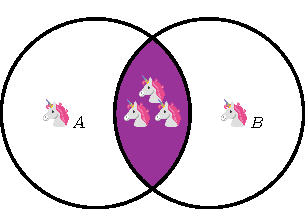
\includegraphics{images/horse_venn.pdf}
    \caption{Horses $A$ and $B$, with all the rest of the horses lying in the violet region common to both sets.}
    \label{fig:horse}
\end{figure}




\subsection*{Question 3: Insertion Sort (6+4=10 points)}

Recall the {\sc Insertion-Sort} algorithm discussed in the lecture:
\begin{code}
	{\sc Insertion-Sort}$(A,n)$\\
	1. \> \For $j=2$ \To $n$\\
	2. \> \> $key=A[j]$\\
	3. \> \> $i=j-1$\\
	4. \> \> \While $i>0$ and $A[i]>key$\\
	5. \> \> \> $A[i+1]=A[i]$\\
	6. \> \> \> $i=i-1$\\
	7. \> \> $A[i+1]=key$
\end{code}

\noindent
In the lecture, you have seen a correctness proof of the algorithm based on the following loop invariant for the (outer) for loop:
\begin{itemize}
	\item Let $A_j[1,\ldots,n]$ denote the array at the beginning of iteration $j$ (end of iteration $j-1$). We have that $A_j[1,\ldots,j-1]$ stores the same values as $A[1,\ldots,j-1]$ but in sorted order, while $A_j[\ell] = A[\ell]$ for $j \leq \ell \leq n$. 
\end{itemize}
In this problem, you will fill in a bit more detail in the proof, by also introducing a loop invariant for the (inner) while loop. You will use the following loop invariant:
\begin{itemize}
	\item Let $A_{j,i}[1,\ldots,n]$ denote the array at the beginning of iteration $i$ of the inner loop (for $0 \leq i \leq j-1$). 
    Then:
    \begin{itemize}
        \item If the loop executes with value $i+ 1$, then 
        \begin{enumerate}[nosep]
		\item $A_{j,i}[1,\ldots,i] = A_j[1,\ldots,i]$, and
		\item If $i+2 \leq j$, then $A_{j,i}[i+2,\ldots,j] = A_j[i+1,\ldots,j-1]$ and $A_j[j] < A_{j,i}[i+2]$.
	\end{enumerate}
 \item Otherwise (if the while loop terminates before reaching value $i + 1$), then $A_{j,i} = A_{j,i+1}$.
    \end{itemize}

\end{itemize}

Solve the following tasks:
\begin{enumerate}
	\item Prove the while loop invariant above using induction over $i$. Start your base case at $i=j-1$ and use backwards induction to show that the claim holds for all smaller $i$. (Prove this for an arbitrary value of $j$,
 where $1 \leq j \leq n$.)
	
\begin{solution}   INSERT YOUR SOLUTION HERE   \end{solution}
	
	\item Use the inner loop invariant to show the induction step of the outer loop invariant.
	
\begin{solution}   INSERT YOUR SOLUTION HERE   \end{solution}
	
\end{enumerate}


%\lhead{\textbf{Basic Algorithms, Fall 2024 \\ CSCI-UA.0310-001}}
\chead{\Large{\textbf{Homework 2}}}
\def\lc{\left\lceil}   
\def\rc{\right\rceil}
\rhead{\textbf{Instructor: Rotem Oshman \\
Ishan Pranav}}
\runningheadrule
\firstpageheadrule
\cfoot{}
Collaborated with Crystal Huang and Sewon Kim. See \href{https://en.wikipedia.org/wiki/Master_theorem_(analysis_of_algorithms)}{Master theorem (analysis of algorithms) -- Wikipedia}.
\subsection*{Question 1}
$f=\mathcal{O}(g)$ is defined for functions $f$ and $g$ (both from $\mathbb{N}$ to $\mathbb{N}$) to mean that exist a positive constant $C$ such that for sufficiently large $n$, $f(n)\leq C\cdot g(n)$. A bit more formally, there exist positive constants $n_0$ and $C$ such that:
$$f(n)\leq C\cdot g(n) \ \text{ for all } n\geq n_0.$$
For each of the following statements either prove the statement if it is true or otherwise provide a counter-example and justify why your counterexample is indeed a counterexample:
\begin{enumerate}
\item If $f=\mathcal{O}(g)$ then $g=\mathcal{O}(f)$.

\textit{Counterexample. }Consider $f(n)=n$ and $g(n)=n^2$. Now $n\leq 1\cdot n^2$ for all $n\geq 2$. There exist positive constants $n_0=2$ and $C=1$ such that $f(n)\leq C\cdot g(n)$ for all $n\geq n_0$, therefore $f=\mathcal{O}(g)$.

Assume, for the sake of contradiction, that $g=\mathcal{O}(f)$. Then there exist constants $n_0'$ and $C'$ for which $g(n)\leq C'\cdot f(n)$ for all $n\geq n_0'$. This implies that there exists a constant $\lim_{n\to\infty}{\frac{g(n)}{f(n)}}$. However, substituting $f$ and $g$ gives $\lim_{n\to\infty}{\frac{n^2}{n}}$, which is unbounded. This contradicts the hypothesis. We conclude that for $f(n)=n$ and $g(n)=n^2$, we have $g\neq\mathcal{O}(f)$.

Hence, the claim that if $f=\mathcal{O}(g)$, then $g=\mathcal{O}(f)$, is false.$~\square$
\item If $f=\mathcal{O}(g)$ and $g=\mathcal{O}(f)$ and $\forall n, f(n)>g(n)$ then $f-g=\mathcal{O}(1)$.

\textit{Counterexample. }Consider $f(n)=2n$ and $g(n)=n$.

Now $2n\leq\frac{1}{2}n$ for all $n\geq 1$. There exist positive constants $n_0=1$ and $C=\frac{1}{2}$ such that $f(n)\leq C\cdot g(n)$ for all $n\geq n_0$, therefore $f=\mathcal{O}(g)$.

Next, $n\leq\frac{1}{2}\cdot 2n$ for all $n\geq 1$. There exist positive constants $n_0'=1$ and $C'=\frac{1}{2}$ such that $g(n)\leq C'\cdot f(n)$ for all $n\geq n_0'$, therefore $g=\mathcal{O}(f)$.

Of course, $2n>n$ for all $n$, therefore $f(n)>g(n)$ for all $n$.

Assume, for the sake of contradiction, that $f-g=\mathcal{O}(1)$. Then there exist positive constants $n_0''$ and $C''$ such that $f(n)-g(n)\leq C''\cdot 1$ for all $n\geq n_0''$. This implies that there exists a constant  $\lim_{n\to\infty}\left[f(n)-g(n)\right]$. However, substituting $f$ and $g$ gives $\lim_{n\to\infty}{[2n-n]}$, which is unbounded. This contradicts the hypothesis. We conclude that for $f(n)=2n$ and $g(n)=n$, we have $f-g\neq\mathcal{O}(n)$.

Hence, the claim that if $f=\mathcal{O}(g)$ and $g=\mathcal{O}(f)$, and for all $n$, we have $f(n)>g(n)$, then $f-g=\mathcal{O}(1)$, is false.$~\square$
\item If $f=\mathcal{O}(g)$ and $g=\mathcal{O}(f)$ then $\frac{f}{g}=\mathcal{O}(1)$.

\textit{Proof. }Suppose $f=\mathcal{O}(g)$ and $g=\mathcal{O}(f)$. Then there exist positive constants $n_0,n_0',C$ and $C'$ such that $f(n)\leq C\cdot g(n)$ for $n\geq n_0$ and $g(n)\leq C'\cdot f(n)$ for $n\geq n_0'$. Observe
\begin{align*}
f(n)\leq C\cdot g(n).
\end{align*}
\begin{align*}
\frac{f(n)}{g(n)}\leq C\cdot\frac{g(n)}{g(n)}\leq C.
\end{align*}
There exist positive constants $n_0$ and $C$ for which $\frac{f(n)}{g(n)}\leq C\cdot 1$ for all $n\geq n_0$. Therefore, $\frac{f}{g}=\mathcal{O}(1)$.$~\square$
\end{enumerate}
\newpage
\subsection*{Question 2}

Consider the following functions:
\begin{multicols}{3}
\begin{description}
    \item a) $\left(\frac{1}{2}\right)^n + 3 n^{17}$
    \item b) $2^{n+\log_2 n}$
    \item c) $2^{4n}$
    \item d) $\sqrt{n^2+n^4}$
    \item e) $\frac{n^8 - n^7}{24}$
\end{description}
\end{multicols}

\begin{enumerate}
    \item For each of the above functions $f(n)$, find a ``canonical'' function $g(n)$ such that $f(n) = \Theta(g(n))$. By canonical we mean that $g$ should be of the form $g(n) = a^n n^b \log^c n$ for constants $a\ge 1$ and $b,c\ge 0$. For example,  $3200n + 2n^2 \log^{24} (n^2) = \Theta(n^2\log^{24} n)$.

\begin{solution}
\begin{enumerate}
\item$\left(\frac{1}{2}\right)^n+3n^{17}=\Theta(n^{17})$. As $n\to\infty$, we have $\left(\frac{1}{2}\right)^n\to 0$ and $3n^{17}\to\infty$. We have the asymptotically dominant term $3n^{17}$; ignoring constants gives $\Theta(n^{17})$.
\item$2^{n+\log_2{n}}=\Theta(n\cdot2^n)$. We have $2^{n+\log_2{n}}=2^n\cdot2^{\log_2{n}}=n\cdot 2^n$.
\item$2^{4n}=\Theta(16^n)$. We have $2^{4n}=\left(2^4\right)^n=16^n$.
\item$\sqrt{n^2+n^4}=\Theta(n^2)$. As $n\to\infty$, the $n^4$ term dominates $n^2$. Ignoring the dominated term, we have $\sqrt{n^4}=n^2$, giving $\Theta(n^2)$.
\item$\frac{n^8-n^7}{24}=\Theta(n^8)$. As $n\to\infty$, the $n^8$ term dominates $n^7$; ignoring constants gives $\Theta(n^8)$.
\end{enumerate}
\end{solution}
\item Based on your answers from above, sort the functions above in asymptotically increasing order. Are there any two functions with the same order of growth? If yes, which ones?
\begin{solution}
In increasing order of asymptotic growth, we have (d), (e), (a), (b), and (c). None of the functions have the same order of growth. We know (b) is greater than (c) because $\lim_{n\to\infty}{\frac{16^n}{n\cdot 2^n}}$ is unbounded.
\end{solution}
\end{enumerate}
\newpage
\subsection*{Question 3}
\label{question:3}
In this problem, we will solve the following recurrence using the \textbf{substitution method} (i.e., induction). Assume $T(1)=0,\; T(2)=1$ and that the recurrences below define $T(n)$ for $n>2$:
\begin{align}
T(n) = T\Big(\frac{n}{3}\Big)+T\Big(\frac{2n}{3}\Big)+1\;. \label{eq:recurrence}
\end{align}

You do not need to worry about the $n/3$ and $2n/3$ terms in~\eqref{eq:recurrence} being fractions. 

\begin{enumerate}
\item Try $T(n) = \sqrt{n}$. Does the recurrence hold? You may ignore the base cases ($n=1$ and $2$) and only look at whether $T(n)$ satisfies Eq.~\eqref{eq:recurrence}. Is the RHS bigger than the LHS? Show your calculations.
\textit{Counterexample. } Consider $T(n)=\sqrt{n}$.
\begin{align*}
\sqrt{n}&\stackrel{?}{=}\sqrt{\frac{n}{3}}+\sqrt{\frac{2n}{3}}+1\\
&\stackrel{?}{=}\frac{1+\sqrt{2}}{3}\sqrt{n}+1\\
&<\frac{1+\sqrt{2}}{3}\sqrt{n}+1.
\end{align*}
Taking $n=3$ as a counterexample, we have $2+\sqrt{2}\neq\sqrt{3}$.

The right-hand side is greater than the left-hand side, so the recurrence does not hold.
\item Try $T(n) = n$. Does the recurrence hold? You may ignore the base cases ($n=1$ and $2$) and only look at whether $T(n)$ satisfies Eq.~\eqref{eq:recurrence}. Is the RHS bigger than the LHS? Show your calculations.
\textit{Counterexample. } Consider $T(n)=n$.
\begin{align*}
n&\stackrel{?}{=}\left(\frac{n}{3}\right)+\left(\frac{2n}{3}\right)+1\\
n&\stackrel{?}{=}n+1\\
n&<n+1.
\end{align*}
Taking $n=3$ as a counterexample, we have $3<4$.

The right-hand side is greater than the left-hand side, so the recurrence does not hold.
\item Try $T(n) = n^2$. Does the recurrence hold? You may ignore the base cases ($n=1$ and $2$) and only look at whether $T(n)$ satisfies Eq.~\eqref{eq:recurrence}. Is the RHS bigger than the LHS? Show your calculations.
\textit{Counterexample. } Consider $T(n)=n^2$.
\begin{align*}
n^2&\stackrel{?}{=}\left(\frac{n}{3}\right)^2+\left(\frac{2n}{3}\right)^2+1\\
n^2&\stackrel{?}{=}\frac{5}{9}n^2+1\\
n^2&>\frac{5}{9}n^2+1.
\end{align*}
Taking $n=3$ as a counterexample, we have $9>6$.

The left-hand side is greater than the right-hand side, so the recurrence does not hold.
\end{enumerate}
Among parts $1$ to $3$, which choice of $T(n)$ ``almost'' satisfied recurrence~\eqref{eq:recurrence}? That is, for which choice of $T(n)$ was the left-hand side \emph{almost equal} to the right-hand side of~\eqref{eq:recurrence}? Reflect on this question because it would help solve the next part.\\

\textit{Among parts 1 to 3, the choice $T(n)=n$ almost satisfies the recurrence. }

\begin{enumerate}[resume]
\item Let $T(n) = n^p + c$ for some $c \in \mathbb{R}$, and $p > 0$ and solve for $p$ and $c$. Based on the $p$ and $c$ you obtained, prove your result formally using the substitution method. (Note that parts $1$-$3$ correspond to $c=0$ and $p=1/2,p=1,p=2$, respectively.)\\
\\

\textit{Proof. }Let $T(n)=n^p+c$ for $c\in\mathbb{R}$ and $p>0$. We will show that $T(n)=n-1$ satisfies the recurrence (that is, we will demonstrate that the recurrence holds for $c=-1$ and $p=1$). Observe
\begin{align*}
T(n)&=T\left(\frac{n}{3}\right)+T\left(\frac{2n}{3}\right)+1\\
&=\left(\frac{n}{3}-1\right)+\left(\frac{2n}{3}-1\right)+1\\
&=n-1\\
&=n^1+(-1).
\end{align*}
Therefore $T(n)=n-1$ satisfies the recurrence.$~\square$
\end{enumerate}
\newpage
\subsection*{Question 4: Merge sort}
Recall Merge Sort, in which a list is sorted by first sorting the left and right halves, and then merging the two lists. 
We define the \textit{3-Merge Sort} algorithm, in which the input list is split into $3$
equal length parts (or as equal as possible), each is sorted recursively, and then the three lists are merged to create a final sorted list. 
\begin{enumerate}
\item Write a recurrence for $T(n)$, the worst-case run time for 3-Merge Sort on any input containing $n$ elements.

Let $f(n)$ represent the worst-case running time of the merge operation with an $n$-element input array, where $f(n)=\Theta(n)$. We can write a recurrence for $T(n)$, the worst-case running time for 3-merge sort with an $n$-element input array:

\[T(n)=3T\left(\frac{n}{3}\right)+f(n).\]

\item Solve this recurrence for $T(n)$. Prove your result formally using the substitution method (i.e., induction). For full credit, you'll need to show matching upper and lower bounds.

\textbf{Solution. }

Let $f(n)$ represent the worst-case running time of the merge operation with an $n$-element input array, where $f(n)=\Theta(n)$. We can write a recurrence for $T(n)$, the worst-case running time for 3-merge sort with an $n$-element input array.

Based on our understanding of merge sort, we can guess that $T(n)=\Theta(n\log n)$.

\textbf{Lemma I. }

\textit{Claim. }$T(n)=O(n\log n)$ for $n\geq 3$.

We want to show that there exists a positive constant $c$ for which $T(n)\leq cn\log n$, and we can prove this result for $n\geq 3$ using induction on $n$.

\textit{Basis. }Consider $n=3$. We have $T(3)=f(3)=\Theta(1)$. We can choose $c$ such that $f(3)\leq 3c\log(3)$. There exists a positive constant $c$ where $c\geq\frac{f(3)}{3\log(3)}$. Therefore the argument holds in the basis case.\\

\textit{Hypothesis. }Consider $3<n\leq k$. Assume $T(k)\leq ck\log k$.\\

\textit{Inductive step. }Consider $n=k+1$. Observe
\begin{align*}
T(k)&=3T\left(\frac{k+1}{3}\right)+f(k+1)\\
&=3T\left(\frac{k+1}{3}\right)+\Theta(k+1).
\end{align*}
Since $\frac{k+1}{3}<k$ for all $k>3$, the strong induction hypothesis holds for $n=\frac{k+1}{3}$.
\begin{align*}
T(k)&\leq 3c\left(\frac{k+1}{3}\right)\log\left(\frac{k+1}{3}\right)+\Theta(k+1)\\
&\leq 3c\left(\frac{k+1}{3}\right)\log\left(\frac{k+1}{3}\right)+c'(k+1)\\
&\leq c(k+1)(\log(k+1)-\log(3))+c'(k+1)\\
&\leq c(k+1)\log(k+1)-c(k+1)\log(3)+c'(k+1)\\
&\leq c(k+1)\log(k+1)-(k+1)(c\log(3)-c').
\end{align*}
Choose $c\log(3)-c'\leq 0$ such that $c$ satisfies the basis case. That is, choose $c$ such that $\frac{f(3)}{3\log(3)}\leq c\leq\frac{c'}{\log(3)}$. For $n=k+1$, there exists a positive constant $c$ for which $T(k+1)\leq c(k+1)\log(k+1)$. 

Hence, $T(n)=O(n\log n)$ for $n\geq 3$, by the principle of mathematical induction.\\

\textbf{Lemma II. }

\textit{Claim. }$T(n)=\Omega(n\log n)$ for $n\geq 3$.

Similarly, we want to show that there exists a positive constant $c$ for which $T(n)\geq cn\log n$, and we can prove this result for $n\geq 3$ using induction on $n$.

\textit{Basis. }Consider $n=3$. We can choose $c$ such that $T(3)\geq 3c\log(3)$. We have $T(3)=f(3)=\Theta(1)$. We can choose $c$ such that $f(3)\geq 3c\log(3)$. There exists a positive constant $c$ where $c\leq\frac{f(3)}{3\log(3)}$. Therefore the argument holds in the basis case.\\

\textit{Hypothesis. }Consider $3<n\leq k$. Assume $T(k)\geq ck\log k$.\\

\textit{Inductive step. }Consider $n=k+1$. Observe
\begin{align*}
T(k)&=3T\left(\frac{k+1}{3}\right)+f(k+1)\\
&=3T\left(\frac{k+1}{3}\right)+\Theta(k+1).
\end{align*}
Since $\frac{k+1}{3}<k$ for all $k>3$, the strong induction hypothesis holds for $n=\frac{k+1}{3}$.
\begin{align*}
T(k)&\geq 3c\left(\frac{k+1}{3}\right)\log\left(\frac{k+1}{3}\right)+\Theta(k+1)\\
&\geq 3c\left(\frac{k+1}{3}\right)\log\left(\frac{k+1}{3}\right)+c'(k+1)\\
&\geq c(k+1)(\log(k+1)-\log(3))+c'(k+1)\\
&\geq c(k+1)\log(k+1)-c(k+1)\log(3)+c'(k+1)\\
&\geq c(k+1)\log(k+1)-(k+1)(c\log(3)-c').
\end{align*}
Choose $c\log(3)-c'\geq 0$. That is, choose $c$ such that $\frac{c'}{\log(3)}\leq c\leq\frac{f(3)}{3\log(3)}$. For $n=k+1$, there exists a positive constant $c$ for which $T(k+1)\leq c(k+1)\log(k+1)$. 

Hence, $T(n)=\Omega(n\log n)$ for $n\geq 3$, by the principle of mathematical induction.

\textbf{Proof. }

\textit{Claim. }$T(n)=\Theta(n\log n)$.

From Lemma I, we have $T(n)=O(n\log n)$ for $n\geq 3$.

From Lemma II, we have $T(n)=\Omega(n\log n)$ for $n\geq 3$.

Ergo $T(n)=\Theta(n\log n)$ for $n\geq 3$.$~\square$
\end{enumerate}
\newpage

\subsection*{Honors Question 1}
{\bf (**)}
Solve the following recurrences (assume $T(1)=T(2)=1$ and that the recurrences below define $T(n)$ for $n>2$). In all cases, you must prove the correctness of your solution. It is good enough to get an answer $f(n)$ such that $T(n)=\Theta(f(n))$.

\begin{enumerate}
\item$T(n)=2T(\lc\sqrt{n}\rc)+\log_2 n$.\\

\textit{Claim. }$T(n)=2T(\lc\sqrt{n}\rc)+\log_2n=\Theta(\log n\log^2 n)$.\\

\textit{Proof. }Let $S(n)=T(2^n)$ for $n>0$. Observe
\begin{align*}
S(n)&=T(2^n)\\
&=2T\lc\sqrt{2^n}\rc+\log_2{2^n}\\
&=2T\lc\sqrt{2^n}\rc+n\\
&=2S\left(\frac{n}{2}\right)+n.
\end{align*}

We can apply the master theorem for divide-and-conquer recurrences. We have a recurrence $S$ of the form $S(n)=2S\left(\frac{n}{2}\right)+n$. The critical exponent is $c^*=\log_2(2)=1$. Note $n=\Theta(n^{c^*}\log_2^0n)$. Therefore, Case II of the master theorem gives
\begin{equation*}
S(n)=\Theta(n^{c^*}\log_2^{0+1}n)=\Theta(n\log_2 n).
\end{equation*}
By construction, $S(n)=T(2^n)$, therefore
\begin{align*}
T(n)&=S(\log_2n)\\
&=\Theta(\log_2n\log_2\log_2n)\\
&=\Theta(\log_2n\log_2^2n).
\end{align*}
Ergo $T(n)=\Theta(\log n\log^2n)$.$~\square$
\item $T(n)=\lc\sqrt{n}\rc T(\lc\sqrt{n}\rc)+n$.\\

\textit{Claim. }$T(n)=\lc\sqrt{n}\rc T(\lc\sqrt{n}\rc)+n=\Theta(n\log\log n)$.\\

\textit{Proof. }
Let $S(n)=T(2^n)$ for $n>0$. Observe
\begin{align*}
S(n)&=T(2^n)\\
&=\lc\sqrt{2^n}\rc T\left(\lc\sqrt{2^n}\rc\right)+2^n\\
&=2^{\frac{n}{2}}T\left(2^{\frac{n}{2}}\right)+2^n\\
\frac{S(n)}{2^n}&=\frac{2^{\frac{n}{2}}T\left(2^{\frac{n}{2}}\right)}{2^n}+1.\\
&=\frac{T\left(2^{\frac{n}{2}}\right)}{2^{\frac{n}{2}}}+1.
\end{align*}
Let $R(n)=\frac{S(n)}{2^n}=\frac{T\left(2^{\frac{n}{2}}\right)}{2^{\frac{n}{2}}}+1$ for $n>0$. Observe
\begin{align*}
R(n)=R\left(\frac{n}{2}\right)+1.
\end{align*}
We can apply the master theorem for divide-and-conquer recurrences. We have a recurrence $R$ of the form $R(n)=1\cdot R\left(\frac{n}{2}\right)+1$. The critical exponent is $c^*=\log_2(1)=0$. Note $1=\Theta(n^{c^*}\log_1^0 n)$. Therefore, Case II of the master theorem gives
\begin{equation*}
R(n)=\Theta(n^{c^*}\log_2^{0+1}n)=\Theta(\log_2n).
\end{equation*}
By construction, $R(n)=\frac{S(n)}{2^n}$, therefore $S(n)=2^nR(n)$. By construction $S(n)=T(2^n)$, therefore
\begin{align*}
T(n)&=2^{\log_2n}R(\log_2n)\\
&=nR(\log_2n)\\
&=n\Theta(\log_2n)\\
&=\Theta(n\log_2\log_2n).
\end{align*}
Ergo $T(n)=\Theta(n\log\log n)$.$~\square$
\end{enumerate}
\newpage
\subsection*{Honors Question 2:}
{\bf (***)} Solve the following recurrence relation
\begin{equation*}
T(n)=8T\left(n/4\right)+n^2,~T(1)=1.
\end{equation*}
\emph{exactly} using the following steps.
\begin{enumerate}
\item %\disppoints{2}
Transform $T(n)$ into an equivalent	recurrence of the form $S(k) = a S(k-1) + f_1(k)$. Do not forget to specify the base case.
\begin{solution}
Let $T(1)=1$ and $T(n)=8T\left(\frac{n}{4}\right)+n^2$ for $n>1$. Define $S(k)=T(4^k)$ for $k>0$. Observe
\begin{align*}
S(k)&=T(4^k)\\
&=8T\left(\frac{4^k}{4}\right)+(4^k)^2\\
&=8T(4^{k-1})+{16}^k.
\end{align*}
\end{solution}
\item %\disppoints{2}
Transform $S(k)$ into an equivalent	recurrence of the form $G(k) = G(k-1) + f_2(k)$. Do not forget to specify the base case.
\begin{solution}
\end{solution}
	
	\item %\disppoints{2}
	Solve $G(k)$ exactly by expanding the sum.
	
\begin{solution}   INSERT YOUR SOLUTION HERE   \end{solution}

	\item %\disppoints{2}
	Substitute back to solve for $T(n)$.
	
\begin{solution}   INSERT YOUR SOLUTION HERE   \end{solution}
\end{enumerate}


\lhead{\textbf{Basic Algorithms, Fall 2024 \\ CSCI-UA.0310-001}}
\chead{\Large{\textbf{Homework 3}}}
\def\lc{\left\lceil}   
\def\rc{\right\rceil}
\rhead{\textbf{Instructor: Rotem Oshman \\ Name: Ishan Pranav}}
\runningheadrule
\firstpageheadrule
\cfoot{}
Collaborated with Crystal Huang.
\subsection*{Question 1: Insertion Sort vs QuickSort}

Recall that in the worst case the running time of (non-randomized) {\sc QuickSort}, that uses the last element as the pivot, and {\sc InsertionSort} are $\Theta(n^2)$. Refer to the lecture notes for the {\sc QuickSort} implementation.

\begin{enumerate}
    \item Give an example of an array of length $n$ where both take time $\Omega(n^2)$. Justify your answer.  
\begin{solution}
Let $A[1,\dots n]$ be an $n$-element array where $A[i]\geq A[i+1]$ for all $1\leq i<n$.\\
\end{solution}
    \item Give an example of an array of length $n$ where (non-randomized) {\sc QuickSort} runs in $\Omega(n^2)$ but {\sc Insertion-Sort} runs in time $O(n)$. Justify your answer. 
\begin{solution}
Let $A[1,\dots n]$ be an $n$-element array where $A[i]\leq A[i+1]$ for all $1\leq i<n$.
\end{solution}
\end{enumerate}
\subsection*{Question 2: Fast Exponentiation}
In this problem, you will design an algorithm to compute $2024^n$ given $n \in \mathbb{N}$ as input. In each case, prove the correctness of your algorithm, and an upper bound on the number of multiplications used.
\begin{enumerate}
    \item Using $n-1$ many multiplications.
\begin{solution}
{\sc NaiveExponentiation}($n$) where $n\in\mathbb{N}$:
\begin{itemize}
\item if $n=1$, then return $2024$;
\item otherwise, return the product $2024~\times~${\sc NaiveExponentiation}($n-1$).
\end{itemize}
\textbf{Proof of correctness. }

\textit{Claim. }{\sc NaiveExponentiation}($n$)$~=2024^n$. We can demonstrate the claim by induction on $n$.

\textit{Basis. }Consider $n=1$. Since $n=1$, we have {\sc NaiveExponentiation}($n$)$~=2024=2024^1$. The claim holds in the base case.

\textit{Hypothesis. }Consider $n=k$ where $k>1$. Assume that {\sc NaiveExponentiation}($k$)$~=2024^k$.

\textit{Inductive step. }Consider $n=k+1$. Then

{\sc NaiveExponentiation}($k+1$)$~=2024~\times~${\sc NaiveExponentiation}($(k+1)-1$). That is,

{\sc NaiveExponentiation}($k+1$)$~=2024~\times~${\sc NaiveExponentiation}($k$).

By the inductive hypothesis, we have {\sc NaiveExponentiation}($k$)$~=2024^k$. Thus

{\sc NaiveExponentiation}($k+1$)$~=2024\times2024^k$. Ergo,

{\sc NaiveExponentiation}($k+1$)$~=2024^{k+1}$, thus completing the inductive step.

Hence, by the principle of mathematical induction, the {\sc NaiveExponentiation} algorithm produces the correct result for all $n\in\mathbb{N}$.$~\square$\\

\textbf{Proof of performance. }

\textit{Claim. }{\sc NaiveExponentiation}($n$) uses at most $n-1$ multiplications. We can demonstrate the claim by induction on $n$.

\textit{Basis. }Consider $n=1$. Since $n=1$, the number of multiplications is $0=1-1\leq n-1$. The claim holds in the base case.

\textit{Hypothesis. }Consider $n=k$ where $k>1$. Assume that {\sc NaiveExponentiation}($k$) uses at most $k-1$ multiplications.

\textit{Inductive step. }Consider $n=k+1$. Then the number of multiplications is $1$, plus the number of multiplications used by {\sc NaiveExponentiation}($(k+1)-1$). That is, $1$ plus the number of multiplications used by {\sc NaiveExponentiation}($k$). By the inductive hypothesis, the number of multiplications used by {\sc NaiveExponentiation}($k$) is at most $k-1$. Therefore, the number of multiplications used by {\sc NaiveExponentiation}($k+1$) is at most $1+(k-1)=(k+1)-1$, thus completing the inductive step.

Hence, by the principle of mathematical induction,the {\sc NaiveExponentiation} algorithm uses at most $n-1$ multiplications for all $n\in\mathbb{N}$.$~\square$
\textit{}
\end{solution}    
    \item Using $O(\log_2 n)$ many multiplications, assuming $n$ is a power of $2$, i.e., $n=2^k$.
\begin{solution}

\end{solution}
    
    \item Using $O(\log_2 n)$ many multiplications for \emph{any} $n$ (not necessarily a power of $2$).
\begin{solution}   INSERT YOUR SOLUTION HERE   \end{solution}
\end{enumerate}
\subsection*{Question 3: Close to Sorted}
Suppose you are given a list $A$ of $n$ distinct numbers. You are guaranteed that this list is `close to sorted' in the following sense: if $A_{\text{sorted}}$ denotes the list fully sorted in increasing order, then $A_{\text{sorted}}$ differs from $A$ in at most $\log_2 n$ many positions. Intuitively, this says that at most $\log_2 n$ elements are out of place in the original list. For instance, in the list 
\[
(2,5,9,11,20,14,15,12,25,30)
\]
only two elements are out of place (20 and 12), since after sorting, we get 
\[
(2,5,9,11,12,14,15,20,25,30) \;.
\]
The following exercises will ultimately lead to an algorithm which sorts $A$ in time $O(n)$~\footnote{Note that sorting algorithms take $O(n\log n)$ time without any assumptions on the inputs. Here, we are able to get the faster $O(n)$ run-time by \emph{assuming} that the input array $A$ is already close to being sorted.}. Answer each exercise. \textbf{Don't forget to read the hints!}

\begin{enumerate}
    \item (Warm up) Prove that the leftmost (first) out of place element must be too big (not too small) for its place.
\begin{solution}
\textit{Claim. }Let $k$ represent the position of the leftmost out-of-place element in $A$.

\textit{Proof. }Assume, for the sake of contradiction, that $k$ is too small for its position. Since $A[k]$ is too small for its position, we know $k>1$. Otherwise, if $k=1$, it could not be too small for its position. Of course, since $A[k]$ is too small for its position, $A[k]<A[k-1]$.

This implies that $A[k-1]>A[k]$, meaning that $A[k-1]$ is too big for its place. $A[k-1]$ is out of place and $k-1<k$. Therefore, $A[k-1]$ is out of place and \textit{further left} than $A[k]$. This contradicts the hypothesis that $A[k]$ is the leftmost out-of-place element in $A$.

We conclude that the leftmost out-of-place element in $A$ must not be too small for its place. Hence, the leftmost out-of-place element in $A$ must be too big for its place.
\end{solution}
    
    \item Suppose we construct a stack $S$ as follows: We go through $A$ from left to right, pushing elements one by one into $S$ as long as the next element from $A$ is larger than the top element $s$ of the stack so far. If at any step $i$ the element $A[i]$ which we are currently considering in $A$ is smaller than $s$, we instead pop $s$ from $S$ and continue.
    This idea is described in the pseudo code below:
    
    \begin{minipage}{\linewidth}
    \begin{algorithm}[H]
    \label{incsubseq}
    \caption{Construct increasing subsequence $S$}
    \begin{algorithmic}
    \REQUIRE $A$ and an empty stack $S$.
    \ENSURE $S$ representing an increasing subsequence of $A$
    \STATE $n \leftarrow \text{len}(A)$
    \FOR {$i = 1 \text{ to } n$}
        \IF {$S$ is empty \OR $S.\text{topElement}() \leq A[i]$}
        \STATE $S.\text{push}(A[i])$
        \ELSE 
        \STATE $S.\text{pop}()$
        \ENDIF
    \ENDFOR
    \STATE \RETURN $S$
    \end{algorithmic}
    \end{algorithm}
    \end{minipage}
    
    \smallskip
    If $A$ is initially $(2,5,9,11,20,14,15,12,25,30)$, what will $S$ be after Algorithm 1 has run?

\begin{solution}   INSERT YOUR SOLUTION HERE   \end{solution}

    
    
    \item Prove that $S$ is an increasing subsequence of $A$ (the elements of the output stack are increasing from bottom to top).

\begin{solution}   INSERT YOUR SOLUTION HERE   \end{solution}
    
    
    \item Prove that $S$ contains all elements of $A$ except at most $2\log_2 n$. (Hint: show that every time we leave out a pair of elements (the ``else'' case) at least one of them must have been an out of place element.)

\begin{solution}   INSERT YOUR SOLUTION HERE   \end{solution}

    
    \item Use the previous statements to design and prove the correctness and run-time of an algorithm to sort the nearly sorted array in time $O(n)$. 
    
    \hint{Suppose you could split $A$ into a large sorted subsequence and only a few remaining unsorted elements in time $O(n)$. (This is what parts 3 and 4 show.) Now think of the ``Merge'' subroutine in Merge Sort.}

\begin{solution}   INSERT YOUR SOLUTION HERE   \end{solution}
\end{enumerate}





    



\subsection*{Honors Question: The Counterfeit Gem}
Suppose you strike up a relationship with a jeweler and get a bulk deal on $n$ diamonds. However, you were warned beforehand that one (and only one) of the diamonds is a convincing fake, and the only difference between it and the real gems is that the fake one's weight is different, while all real ones have the same weight. Luckily, you have a balance scale at home, which can test two (disjoint) subsets of the diamonds and tell us which is lighter. 

\begin{enumerate}
    \item $(**)$ Assume that you know that the fake one is lighter. Give an algorithm that finds the counterfeit gem in $O(\log n)$ uses of the scale. Justify the correctness and time complexity of your proposed algorithm.

\begin{solution}   INSERT YOUR SOLUTION HERE   \end{solution}

    \item $(****)$ Now consider the general case where you only know it has a different weight from the real ones. What can you do in this case? Can you still do it with $O(\log n)$ measurements? For concrete numbers, consider $n=12$ and show how you can identify the fake one only using the scale $3$ times.

\begin{solution}   INSERT YOUR SOLUTION HERE   \end{solution}
\end{enumerate}


  %\lhead{\textbf{Basic Algorithms, Fall 2024 \\ CSCI-UA.0310-001}}
\chead{\Large{\textbf{Homework 4}}}
\def\lc{\left\lceil}   
\def\rc{\right\rceil}
\rhead{\textbf{Instructor: Rotem Oshman \\ Name: Ishan Pranav}}
\runningheadrule
\firstpageheadrule
\cfoot{}

\newcommand{\True}{\mathtt{true}}
\newcommand{\False}{\mathtt{false}}

\subsection*{References}

Collaborated with Crystal Huang.

\subsection*{Question 1: $k$-th Smallest Element from Two Lists}

Suppose you are given two \emph{sorted} lists $A[1,\ldots,n]$ and $B[1,\ldots,m]$ of size $n$ and $m$, respectively. Give an $O(\log k)$ algorithm to find the $k$-th
smallest element in $A \cup B$, i.e., of the combination of the two arrays. For simplicity, you can assume $k \leq \min(m,n)$. Justify the correctness and running time of your algorithm. 

\begin{solution}\\

\noindent\textbf{Algorithm. }{\sc FindIndex}($A,B,k$) where $A[1,\dots,n],B[1,\dots,m]$ are sorted lists and $k\in\mathbb{N}$ where $k\leq\min(n,m)$. That is, for all $1\leq i<n$, we have $A[i]\leq A[i+1]$, and for all $1\leq j<m$, we have $B[j]\leq B[j+1]$:
\begin{itemize}
\item if $n=0$, then return $B[k]$;
\item if $m=0$, then return $A[k]$;
\item if $k=1$, then return $\min(A[1],B[1])$;
\item otherwise, for $k>1$, compute $i\leftarrow\left\lfloor\frac{k}{2}\right\rfloor$. Then:
\begin{itemize}
\item if $A[i]\leq B[i]$, then return {\sc FindIndex}($A[i+1,\dots,n],B[1,\dots,m],k-i$);
\item otherwise, return {\sc FindIndex}($A[1,\dots,n],B[i+1,\dots,m],k-i$).
\end{itemize}
\end{itemize}

\noindent\textbf{Proof I.}

\noindent\textit{Claim. }For all sorted lists $A[1,\dots,n],B[1,\dots,m]$ and all $k\leq\min(n,m)$, {\sc FindIndex}($A,B,k$) returns $C[k]$, where $C=~${\sc Merge}($A,B$), the result of the well-known {\sc Merge} algorithm. That is, {\sc FindIndex}($A,B,k$) returns the $k$-th element of the sorted list that contains all elements of sorted lists $A$ and $B$ (and no other elements). Note $k\geq 1,m\geq 0,n\geq 0$.

\begin{itemize}
\item Suppose $n=0$. Then $m\geq 1$. Consider $C[1,\dots,m]$, the result of merging $A$ and $B$. Since $n=0$, we know $C=B$. For all $k\in\mathbb{N}$, {\sc FindIndex}($A,B,k$) returns $B[k]=C[k]$. Thus, when $n=0$, the claim holds for all $k\in\mathbb{N}$.
\item Suppose $m=0$. Then $n\geq 1$. Consider $C[1,\dots,n]$, the result of merging $A$ and $B$. Since $m=0$, we know $C=A$. For all $k\in\mathbb{N}$, {\sc FindIndex}($A,B,k$) returns $A[k]=C[k]$. Thus, when $m=0$, the claim holds for all $k\in\mathbb{N}$.
\item Suppose instead $m>0$ and $n>0$. We can demonstrate the claim for $m>0$ and $n>0$ by induction on $k$.\\

\textit{Basis. }Consider $k=1$. Consider also $C[1,\dots,m+n]$, the result of merging $A$ and $B$. The least element in $C$ is either the least element in $A$ or the least element in $B$; specifically, it is the smaller of the least element in $A$ and the least element in $B$. Of course, in this case {\sc FindIndex}($A,B,k$) returns $\min(A[1],B[1])$. Since $A,B$ are sorted lists, $A[1]$ is the least element in $A$ and $B[1]$ is the least element in $B$. Therefore {\sc FindIndex}($A,B,k$) returns the first smallest element in $C$. Since $k=1$, the basis holds for all $A[1,\dots,n],B[1,\dots,m]$.\\

\textit{Hypothesis. }Consider $1<k\leq\ell<\min(n,m)$. Assume that for all sorted lists $A[1,\dots,n]$ and $B[1,\dots,n]$, {\sc FindIndex}($A,B,\ell$) returns the $\ell$-th element of the sorted list that contains all elements of $A$ and $B$ (and no other elements).\\

\textit{Inductive step. }Consider $k=\ell+1$. For all sorted lists $A[1,\dots,n],B[1,\dots,m]$, we have $i=\left\lfloor\frac{\ell+1}{2}\right\rfloor$. Consider $C[1,\dots,m+n]$, the result of merging $A$ and $B$.
\begin{itemize}
\item Suppose $A[i]\leq B[i]$. Since $A$ and $B$ are sorted, and since $A[i]\leq B[i]$, we know that the $(\ell+1)$-th element in $C$ is definitely not within the first $i$ elements of $A$. We can ignore the first $i$ elements in $A$, adjusting our index in the subarray from $\ell+1$ to $\ell+1-i$ (to account for the $i$ elements excluded, which precede it in sorted order).

The result for the new subarray is given by {\sc FindIndex}($A[i+1,\dots,n],B[1,\dots,m],k-i$), which is the return value of the algorithm in this case. By the strong induction hypothesis, the claim holds for this result.
\item Suppose instead $A[i]>B[i]$. Since $A$ and $B$ are sorted, and since $B[i]<A[i]$, we know that the $(\ell+1)$-th element in $C$ is definitely not within the first $i$ elements of $B$. We can ignore the first $i$ elements in $B$, adjusting our index in the subarray from $\ell+1$ to $\ell+1-i$ (to account for the $i$ elements excldued, which precede it in sorted order).

The result for the new subarray is given by {\sc FindIndex}($A[1,\dots,n],B[i+1,\dots,m],k-i$), which is the return value of the algorithm in this case. By the strong induction hypothesis, the claim holds for this result.
\end{itemize}

In all cases, {\sc FindIndex}($A,B,\ell+1$) returns the ($\ell+1$)-th element of the sorted list that contains all elements of $A$ and $B$ (and no other elements), thus completing the inductive step.

Hence, by the principle of mathematical induction, the claim holds for all $k\in\mathbb{N}$ when $m>0$ and $n>0$.
\end{itemize}

We have shown that for all sorted lists $A[1,\dots,n],B[1\dots,m],n\geq 0,m\geq 0,k\in\mathbb{N}$, if $k\leq\min(n,m)$, then {\sc FindIndex}($A,B,k$) returns the $k$-th element of the sorted list that contains all elements of sorted lists $A$ and $B$.$~\square$
\end{solution}
\subsection*{Question 2: Permutations (4+2+2+2+2=12 points)}

Define the notation $[n] = \{1, 2, \ldots, n\}$, and let $S_n$ be the set of all possible permutations of $[n]$. The size of $S_n$ is given by $|S_n|=n!=n\cdot (n-1) \cdots 1$. Recall that $n!=O(n^n)$ and $2^n=O(n!)$. 
Now, each input in $S_n$ can serve as an input for a sorting algorithm. Instead of a perfectly correct sorting algorithm, we will look at a class of algorithms that only produce a sorted result on some of the inputs. More concretely, we say that a sorting algorithm is $\eps$-correct if the algorithm produces the correct result (i.e., produces a sorted array as output) on exactly $\eps$ fraction of the set of inputs in $S_n$. In other words, an $\eps$-correct sorting algorithm is one that produces the correct result on $\eps \cdot (n!)$ possible inputs and produces an incorrect result otherwise.

\begin{enumerate}
    \item Show that for any $0\leq \epsilon\leq 1$, the decision tree of an $\epsilon$-correct comparison-based sorting algorithm must have at least $\epsilon \cdot n!$ leaves. \hint{Recall from the lecture that the output of a comparison-based sorting algorithm is a permutation that prescribes how the input array has to be shuffled to obtain the sorted output. For one of the inputs on which the algorithm is correct, how does the output permutation relate to the input permutation?}
\begin{solution}   INSERT YOUR SOLUTION HERE   \end{solution}
\end{enumerate}

\noindent
In the following, we want to investigate whether lowering $\eps$ can yield a saving in the number of comparisons required by a sorting algorithm. Intuitively if the algorithm only has to be correct on a certain fraction of inputs this should speed up the algorithm. For instance, an algorithm that does not need to be correct at all clearly does not need $\Omega(n \log n)$ comparisons. \hint{Use the number of leaves in the decision tree to derive a lower bound on its height.} 

\begin{enumerate}[resume]
    \item Let $\eps=1/2$. Show that for any constant $C\geq 0$, there is no comparison-based $\eps$-correct sorting algorithm that can sort using less than $C \cdot n$ comparisons. This shows that taking $\eps=1/2$ does not help us reduce the number of comparisons to linear. 
\begin{solution}   INSERT YOUR SOLUTION HERE   \end{solution}

    \item Consider $\eps=1/n$. In this setting, are we able to achieve a sorting algorithm for $S_n$ with $O(n)$ comparisons? Justify your answer.
\begin{solution}   INSERT YOUR SOLUTION HERE   \end{solution}
    
    \item Consider $\eps=\frac{1}{2^n}$. In this setting, are we able to achieve a sorting algorithm for $S_n$ with $O(n)$ comparisons? Justify your answer.
\begin{solution}   INSERT YOUR SOLUTION HERE   \end{solution}
    
    \item Consider $\eps=\frac{2^n}{n!}$. In this setting, are we able to achieve a sorting algorithm for $S_n$ with $O(n)$ comparisons?
\begin{solution}   INSERT YOUR SOLUTION HERE   \end{solution}
\end{enumerate}



\subsection*{Disjointed Arrays (2+5+3=10 points)}
Let $A[1,\ldots,m]$ and $B[1,\ldots,n]$ be two sorted
arrays each containing distinct elements. Let
$m\leq n$ and $n$ is a multiple of $m$. 
The problem is to determine if the two arrays
are disjointed or not. Two arrays are said
to be disjointed if their intersection is
$\emptyset$. 

\begin{enumerate}
	\item Let us assume that $A$ and $B$ are disjoint.
	We define $C$ as the sorted combination of
	$A$ and $B$, i.e., $C=A\cup B$ and $C$ is sorted. Clearly,
	$|C|=m+n$ because $A\cap B=\emptyset$. Define
	$D$ of length $m+n$ where $D[i]=1$ if $C[i]\in A$ and 0
	otherwise. Give a count of the number of such possible
	arrays $D$. Justify your answer. 

\begin{solution}
For each element $1\leq i\leq m+n$ in $D[1,\dots,m+n]$, the value $D[i]=1$ if $C[i]\in A$, and $0$ otherwise. Since $C=A\cup B$, we know $D[i]=1$ if $C[i]\in A$ or $0$ if $C[i]\in B$.

There are $m+n$ many elements in $D$, and for each element, it is either in $A$ or not in $A$. It is known that there are $n$ elements in $A$, so $n$ of $m+n$ elements must be chosen to be $1$ and the other $m$ elements must be $0$.

Thus, the number of such possible arrays is $\binom{m+n}{n}=\binom{m+n}{m}$.

\end{solution}

	\item We go back to the original problem---we do not know whether $A,B$ are disjoint. Let us assume that $A$ contains 1 element, and $B$ contains 2 elements. 
	
	\begin{itemize}
	\item Draw a comparison-based decision tree for this problem.
	\item You will also present a modification of the above tree
	where you will change the label of every leaf node marked as $\True$ 
	with a corresponding array $D$. 
	\end{itemize}
	
	You will ensure that your decision tree makes 
	the least number of comparisons possible and has
	the shortest height possible. The internal 
	node will be of the form $(i,j)$ which 
	indicates that you are comparing $A[i]$ and $B[j]$. 
	Now, each such internal node will have three children - 
	one corresponding to $A[i]<B[j]$, one corresponding to $A[i]=B[j]$,
	and one corresponding to $A[i]>B[j]$. The leaf
	nodes will contain the values $\True,\False$
	where $\True$ indicates that $A,B$ are disjoint
	and $\False$ indicates the opposite. 
	
\begin{solution}

\end{solution}


	\item Now we look at the general problem, i.e.,
	for any $m,n$. It can be shown that the decision
	tree for this general problem will have every
	leaf node labeled $\True$ correspond with
	a distinct array $D$, as defined in part (a).
	This is in fact a bijective mapping, i.e., every
	leaf node labeled $\True$ has a corresponding array $D$
	and every array $D$ has a corresponding leaf node
	labeled $\True$
	Now, using this and your answer from part (a),
	show that problem has a worst-case lower
	bound of $\Omega(m\log(1+n/m))$.
	\hint{Use: ${a\choose b}\geq (a/b)^b$.}

\begin{solution}   INSERT YOUR SOLUTION HERE   \end{solution}
\end{enumerate}
  %\lhead{\textbf{Basic Algorithms, Fall 2024 \\ CSCI-UA.0310-001}}
\chead{\Large{\textbf{Homework 5}}}
\def\lc{\left\lceil}   
\def\rc{\right\rceil}
\rhead{\textbf{Instructor: Rotem Oshman \\
Name: Ishan Pranav}}
\runningheadrule
\firstpageheadrule
\cfoot{}
\stepcounter{subsection}
\subsection*{References}
Collaborated with Crystal Huang.

\subsection{Fast sorting}

\begin{enumerate}
    \item Assume you are given an array of $n$ integers in the range
    $\{1,\ldots, (\log n)^{\log n}\}$. Show how to sort this array in time
    $O(n\log\log n)$.

\begin{solution}
\textit{Definitions. }Let {\sc RadixSort}($A,b$) denote the well-known radix sorting algorithm that sorts an array of $n$ keys $A[1,\dots,n]$ using radix $b$. By definition, {\sc RadixSort}($A,b$) sorts $A[1,\dots,n]$ in time $\Theta((n+b)\cdot w)$, where $w$ is the maximum key length in $A$.

Let $A^*[1,\dots,n]$  be an $n$-element array where, for all $a\in A^*$, we have $a\in\mathbb{Z}$ and $1\leq a\leq(\log n)^{\log n}$. 

\textit{Claim. }{\sc RadixSort}($A^*,n$) sorts $A^*[1,\dots,n]$ in time $O(n\log\log n)$.

\textit{Proof. }For all $a\in A^*$, the length of $a$ in radix $b$ is $\log_ba$. Thus, for all $a\in A^*$, the length of $a$ in radix $b=n$ is $\log_na$. By construction, the maximum value in $A^*$ is $(\log n)^{\log n}$. Thus $w$, the maximum key length in $A^*$ is
\begin{align*}
w&=\log_b(\log n)^{\log n}\\
&=\log_n(\log n)^{\log n}\\
&=\log n\log_n(\log n)\\
&=\log n\cdot\frac{\log\log n}{\log n}\\
&=\log\log n.
\end{align*}
Now the running time of {\sc RadixSort}($A^*,n$) is
\begin{align*}
\Theta((n+b)\cdot w)&=\Theta((n+n)\cdot\log\log n)\\
&=\Theta(n\log\log n)\\
&=O(n\log\log n).
\end{align*}
Hence, we can sort $A^*[1,\dots,n]$ using {\sc RadixSort}($A^*,n$) in $O(n\log\log n)$ time.$~\square$
\end{solution}
\newpage
\item Assume you are given an array of $n$ integers with many
duplicates, so that you know that there are at most $\log n$
distinct elements in the array. Show how to sort this array in time
$O(n)$ if you can use an arbitrary amount of memory, i.e., arrays of arbitrary sizes).
\begin{solution}\\

\textbf{Axiom I. }Assume that an arbitrarily-sized array can be initialized with all-$0$ values in constant time.

\textbf{Axiom II. }Assume that a dynamically-sized list can be initialized in constant time.

\textbf{Algorithm I. }The well-known algorithm {\sc MergeSort}($L$) where $L$ is an $n$-element list. It is given that {\sc MergeSort} sorts $L$ in time $\Theta(n\log n)$.

\textbf{Algorithm II. }{\sc FrequencySort}($A$) where $A[1,\dots,n]$ is an $n$-element array with at most $\log n$ distinct elements:

Visit each element in $A$ to determine the maximum value $m$.

Initialize an array $B[1,\dots,m]$ where $B[i]=0$ for all $1\leq i\leq m$. 

Initialize also a list of integers $L$ with maximum length $\log n$.

For each element $a\in A$:
\begin{itemize}
\item if $B[a]=0$, then append $a$ to $L$,
\item assign $B[a]\leftarrow B[a]+1$.
\end{itemize}

Perform {\sc MergeSort}($L$).

Let $i\leftarrow 1$.

For each element $\ell\in L$:
\begin{itemize}
\item for $j=1$ to $B[\ell]$:
\begin{itemize}
\item assign $A[i]\leftarrow\ell$,
\item assign $i\leftarrow i+1$.
\end{itemize}
\end{itemize}
\textbf{Proposition I. }

\textit{Claim. }{\sc FrequencySort} sorts $A[1,\dots,n]$.

\textit{Proof. }On each iteration of the loop, $B[a]$ is incremented at the end of the loop body. This means that at the beginning of the loop body if $B[a]=0$, $a$ is unique thus far. So, $a$ is appended to $L$. Thus, $L$ contains the unique elements in $a$. By construction of $A$, the maximum length of $L$ is $\log n$. When the loop completes, $B[a]$ contains the number of times $a$ is found in $A$.

{\sc MergeSort}($L$) sorts $L$, the unique elements in $A$.

The second loop visits each element in the now-sorted list $L$ and uses the frequencies stored in $B$ to reconstruct the original array $A$. For each $\ell\in L$, the inner loop copies the exact number of duplicate elements of $\ell$ that exist in $A$, which is given by $B[\ell]$. The index variable $i$ is incremented to maintain the position in $A$. 

Since each element in $A$ was accounted for, either by adding an element to $L$ or by incrementing an existing value in $B$, we know that by iterating through the $\log n$ values of $L$ and reconstructing $A$ in this way, we visit all $n$ elements in $A$. Since each $\ell=\ell$ and since $L$ is sorted, the elements are copied into $A$ in sorted order.

Consequently, $A$ contains its original elements now in sorted order at the end of the algorithm.$~\square$

\textbf{Proposition II. }

\textit{Claim. }{\sc FrequencySort} executes in $O(n)$ time.

\textit{Proof. }First, the algorithm determines the maximum value in $A$, which is an $O(n)$ process.

Initializing $B$ and $L$ is an $O(1)$ process by Axioms I and II.

For each of the $n$ elements in $A$, comparing $B[a]$ to $0$, appending $a$ to $L$, and incrementing $B[a]$ are all $O(1)$ processes. Thus, the first loop is performed in $O(n)$ time.

Since $L$ contains only the unique values in $A$, the maximum length of $L$ is $\log n$.

From Algorithm I, performing {\sc MergeSort} on $L$ is an $O(\log n\log\log n)$ process.

Initializing $i$ is an $O(1)$ process.

For each of the $\log n$ elements in $L$, the number of inner loop iterations is given by the corresponding frequency in $B$. By construction, the sum of all frequencies is $n$. For the innermost loop body, the total number of iterations is $n$. Assigning $A[i]$ and incrementing $i$ are $O(1)$ processes. Therefore, the second loop is performed in $O(n)$ time.

We conclude that the asymptotic running time of {\sc FrequencySort} is $O(n)+O(\log n\log\log n)+O(1)=O(n)$.$~\square$
\end{solution}
\end{enumerate}
\newpage
\subsection{Rod cutting with cost}
Recall the Rod Cutting problem from the lecture: Suppose we have a rod of length $n$ inches and we also have an array of prices $P$, where $P[i]$ denotes the selling price (\$) of a piece that is $i$ inches long. Using dynamic programming (DP), one can efficiently find the maximal revenue obtained by cutting the rod and selling the individual pieces. 

Suppose now we have to pay a cost of \$1 per cut. Define the \emph{profit} we make as the revenue minus the total cost of cutting. We want an algorithm that finds a way to cut the rod that maximizes our \textbf{profit}. For example, if we have $P = (2,5,6,7)$ and $n=4$, then cutting it into two rods of length $2$ yields optimal profit $9=P[2]+P[2]-1$.

\begin{enumerate}
\item Describe recursive formula $R(i)$ for the maximal profit when having a rod of length $i$. (You can use the values of $P$ inside your formula.) Do not forget the base case and justify the correctness of your formula.
\begin{solution}
\textit{Definitions. }Consider the recursive function $R(i)$ for integers $i>0$:
\begin{align*}
R(i)= 
\begin{cases} 
    0,&i=0;\\
    \max\left(P[i],\underset{1\leq j<i}{\max}\left(P[j]+R[i-j]-1\right)\right)&i>0.
\end{cases}
\end{align*}
\textit{Claim. }For integers $i\geq 0$, the recursive function $R(i)$ computes the maximal profit, in dollars, for a rod with length $i$ inches.

\textit{Proof. }We can demonstrate the claim by induction on $i$.

\textit{Basis. }Consider $i=0$. A $0$-inch rod cannot be sold or cut, so the maximum profit is $\$0$. In this case, $R(0)=0$, so the claim holds in the base case.

\textit{Hypothesis. }Consider $0<i\leq k$. Assume that $R(k)$ computes the maximal profit, in dollars, for a rod with length $k$ inches.

\textit{Inductive step. }Consider $i=k+1$. The maximum profit for a $(k+1)$-inch rod is \textit{either} the revenue obtained by selling that rod without cutting it, or the maximum profit obtainable by cutting it, whichever is greater.

\begin{itemize}
\item Consider the case when we do not cut the rod.Thenthe maximum profit is $P[k+1]$.
\item Consider the cases when we cut the rod. The rod can be cut after each $1$-inch segment from segment $1$ to segment $(k+1)-1$.

For each of these positions $j$, two rods are produced: one of length $j$, and another of length $(k+1)-j$. The maximum profit in this case is the revenue obtained from selling a $j$-inch rod, plus the maximum profit obtainable from the remaining portion of the rod, less the $\$1$ cost of cutting the rod.

By the strong induction hypothesis, $R[(k+1)-j]$ is the maximum profit for the remaining $((k+1)-j)$-inch rod.

The rod should be cut at the position with the largest total profit.
 
In this case, $R(k+1)=\underset{1\leq j<k+1}{\max}\left(P[j]+R[(k+1)-j]-1\right)$, so the claim holds.
\end{itemize}
In all cases, the claim holds.

Hence, by the principle of mathematical induction, $R(i)$ computes the maximal profit, in dollars, for a rod with length $i$ inches.$~\square$
\end{solution}
\item Implement your strategy using top-down DP with memoization.
\begin{solution}\\

\textbf{Environment. }Let {\sc Memo} be a global array which stores the values of the subproblems. Initialize {\sc Memo} with all $0$ values.

\textbf{Algorithm. }{\sc RodCut}($i,P$) for integer $i\geq 0$ and array of prices $P$. {\sc RodCut} returns the maximal profit in dollars for a rod with length $i$ inches:
\begin{itemize}
\item if $i=0$, then return $0$,
\item if {\sc Memo}$[i]\neq 0$, then return {\sc Memo}$[i]$.
\item otherwise,
\begin{itemize}
\item let $a\leftarrow P[i]$,
\item for $j=1$ to $i-1$, assign $a\leftarrow \max(a,P[j]+\textsc{RodCut}(i-j,P)-1)$,
\item assign {\sc Memo}$[i]\leftarrow a$,
\item return $a$.
\end{itemize}
\end{itemize}
\end{solution}
\end{enumerate} 

In the following, we want to implement a solution using \emph{bottom-up} DP, i.e., using an array to store the solutions rather than recursion.
For your DP algorithm, use the name $\textsc{MaxProfit}$ for the (potentially multi-dimensional) array which stores values of the subproblems.
\begin{enumerate}[resume]   
    \item Describe in words what $\textsc{MaxProfit}$ should be and state its dimension.
\begin{solution}\\

\textbf{Environment. }Let {\sc MaxProfit}$[0,\dots,i]$ be a one-dimensional $(i+1)$-element array which stores the values of the subproblems.

{\sc MaxProfit} needs sufficient capacity to contain all subproblems for a rod of length $i$, from the trivial rod of length $0$ to the solution of length $i$.
\end{solution}
\newpage
    \item Implement your solution using bottom-up dynamic programming. 
\begin{solution}\\

\textbf{Algorithm. }{\sc RodCut2}($i,P$) for integer $i\geq 0$ and array of prices $P$. {\sc RodCut2} returns the maximal profit in dollars for a rod with length $i$ inches:

Initialize array {\sc MaxProfit}$[0,\dots,i]$.

Assign {\sc MaxProfit}$[0]\leftarrow 0$.

For $k=1$ to $i$:
\begin{itemize}
\item $a\leftarrow P[k]$,
\item for $j=1$ to $k-1$, assign $a\leftarrow\max(a,P[j]+\textsc{MaxProfit}(k-j)-1)$,
\item {\sc MaxProfit}$[k]\leftarrow a$.
\end{itemize}

Return {\sc MaxProfit}$[i]$.
\end{solution}
\item Justify the run time of your algorithm to compute $\textsc{MaxProfit}$ as a big-$\Theta$ expression.
\begin{solution}\\

\textbf{Axiom.} Assume that an arbitrarily-sized array can be initialized with all-$0$ values in constant time.

\textbf{Proposition. }\textit{Claim. }{\sc RodCut2} executes in $\Theta(n^2)$ time.

\textit{Proof. }First, the algorithm initializes {\sc MaxProfit} and assigns {\sc MaxProfit}$[0]$, which are $\Theta(1)$ by the Axiom.

The outer for loop body executes $i$-many times. For each of the $i$ iterations, assigning $a$ and assigning {\sc MaxProfit}$[k]$ are $\Theta(1)$.

The inner loop body executes $(k-1)$-many times, which is itself dependent on $i$. For each inner loop iteration, assigning $a$ and determining the maximum of two arguments are $\Theta(1)$ operations.

Since the inner and outer loop both depend on $i$, and the innermost loop body only performs constant operations, the overall complexity of the loop is $\Theta(i^2)$.

We conclude that the asymptotic running time of {\sc RodCut2} is $\Theta(i^2)+\Theta(1)=\Theta(i^2)$.$~\square$
\end{solution}
\end{enumerate}
\newpage
\subsection{Subset sum}
Let $A = [a_1, \ldots, a_n]$ be an array of $n$ natural numbers. Given a number $t \in \mathbb{N}$, we say $t$ is a \emph{subset sum} of $A$ if there is a \emph{subset of indices} $S \subseteq \{1,\ldots,n\}$ such that $\sum_{i \in S} a_i = t$. For example, if $A=[1,3,5,7]$ then $12$ is a subset sum of $A$ since $5+7=12$, but $2$ is not. (Note that each value can only be included in the sum at most once.)

We want to design an algorithm that determines whether a given number $t \in \mathbb{N}$ is a subset sum of $A$. Specifically, when given $A = [a_1,\ldots,a_n]$ and $t \in \mathbb{N}$ as input, the algorithm should output $1$ if $t$ is a subset sum of $A$, and $0$ otherwise.
We will use (bottom-up) dynamic programming with a two-dimensional array to solve this problem. The subproblem in your DP algorithm should be $\textsc{SubsetSum}$, which is defined as
\begin{align*}
\textsc{SubsetSum}[i][t] = 
\begin{cases} 
    1 &\text{ if $t$ is a subset sum of the first $i$ elements $A_{1:i}=[a_1,\ldots,a_i]$,} \\
    0 &\text{ otherwise.}
\end{cases}
\end{align*}

Also, let us define $M = \sum_{i=1}^n a_i$, which is the sum of all numbers in $A$. The quantity $M$ may appear in the size of the DP array and the run-time of your algorithm.

\begin{enumerate}
    \item Suppose $A=[2,1,3]$. Fill out the following table for $A$. Note that we define the sum over the empty set to be $0$. The pre-filled entries in the top left corner correspond to $\textsc{SubsetSum}[0][0]=1$ and $\textsc{SubsetSum}[0][1]=0$.
    \begin{table}[H]
        \centering
        \captionsetup{width=.7\linewidth}
        \begin{tabular}{|c|c|c|c|c|c|c|c|}
            \hline
            \backslashbox{$i$}{$t$} & 0 & 1 & 2 & 3 & 4 & 5 & 6\\
            \hline
            0 & 1 & 0 & 0 & 0 & 0 & 0 & 0 \\
            \hline
            1 & 1 & 0 & 1 & 0 & 0 & 0 & 0 \\
            \hline
            2 & 1 & 1 & 1 & 1 & 0 & 0 & 0 \\
            \hline
            3 & 1 & 1 & 1 & 1 & 1 & 1 & 1 \\
            \hline
        \end{tabular}
        \caption{Fill in the entries for $\textsc{SubsetSum}[i][t]$.}
        \label{tab:subset-sum}
    \end{table}

\item In general, what is the size of the DP array containing values for $\textsc{SubsetSum}$?
\begin{solution}
The maximum value for $i$ is $n$ and the minimum value for $i$ is $0$. Similarly, the maximum value for $t$ is $M=\sum_{j=1}^n{a_j}$ (when $i=n$), and the minimum value for $t$ is $0$ (when $i=0$). Therefore, the horizontal $t$-dimension must be $M+1$ and the vertical $i$-dimension must be $n+1$. Thus, the size of the dynamic programming array containing values for {\sc SubsetSum} is $(n+1)\times(M+1)$.
\end{solution}
\item State the base cases for $i=0$, i.e., state all the values for $i=0$.
\begin{solution}
Consider $i=0$. When $i=0$, the first $i$ elements $A_{1:i}=[a_1,\dots,a_i]$ is an empty subset of $A$. The only subset sum that can be made is $0$. Thus, {\sc SubsetSum}$[0][0]=1$ and {\sc SubsetSum}$[0][t]=0$ for all $0<t\leq M$. 
\end{solution}
\item Give and justify the recurrence $\textsc{SubsetSum}$ should satisfy.
\begin{solution}
\textit{Claim. }Let $R$ denote the recurrence for $\textsc{SubsetSum}$. Then
\begin{align*}
R(i,t)=
\begin{cases} 
    1,&i=0\text{ and }t=0,\\
    0,&i=0,\text{ and }t\neq 0,\\
    R(i-1,t),&i\neq 0,t\neq 0,\text{ and }t-a_i<0,\\
    R(i-1,t)\lor R(i-1,t-a_i),&\text{ otherwise.}
\end{cases}
\end{align*}
\textit{Proof. }We can demonstrate the claim for all $0\leq t\leq M$ using induction on $0\leq i\leq n$.

\textit{Basis. }Consider $i=0$. When $i=0$, the first $i$ elements $A_{1:i}=[a_1,\dots,a_i]$ is an empty subset of $A$. The only subset sum that can be made is $0$. Thus, $R(0,0)=1$ and $R(0,t)=0$ for all $0<t\leq M$.

Thus for all $0\leq t\leq M$, the claim holds in the base case.

\textit{Hypothesis. }Consider $0<i\leq k<n$. Assume that $R$ is the recurrence for {\sc SubsetSum} for all $0\leq t\leq M$.

\textit{Inductive step. }Consider $i=k+1$. Let $0\leq t\leq M$. We want to determine if $t$ is a subset sum of $[a_1,\dots,a_{k+1}]$. We can either include $a_{k+1}$ in this subset or not include $a_{k+1}$ in this subset.
\begin{itemize}
\item Suppose $a_{k+1}$ is not included in the subset. Then the result should be $1$ if $t$ is a subset sum of $[a_1,\dots,a_k]$, and $0$ otherwise. By the inductive hypothesis, $R(k,t)$ provides this result.
\item Suppose instead $a_{k+1}$ is included in the subset. If we were able to produce the sum $t-a_{k+1}$ from the first $k$ elements, then the inclusion of $a_{k+1}$ brings the subset sum to $(t-a_{k+1})+a_{k+1}=t$, so it is possible to achieve a subset sum of $t$ using the first $k+1$ elements.

If $t-a_{k+1}<0$, then it is certainly impossible to produce a negative sum using only the natural numbers in $A$, so this case does not apply.

If, however, $t-a_{k+1}\geq 0$, then by the strong induction hypothesis, $R(k,t-a_{k+1})$ gives $1$ if we were able to procue the sum $t-a_{k+1}$ from the first $k$ elements, and $0$ otherwise.

Thus $R(k,t-a_{k+1})$ gives the desired result.
\end{itemize}
If the subset sum $t$ is achievable by including $a_{k+1}$ or by not including $a_{k+1}$, then the result should be $1$, and $0$ otherwise. The logical \textit{or} of the two results above provides this behavior.

This completes the inductive step for all $0\leq t\leq M$.

Hence, by the principle of mathematical induction, we have $R$ as the correct recurrence for {\sc SubsetSum} for all $0\leq t\leq M$, for all $0\leq i\leq n$.$~\square$
\end{solution}
\newpage
\item For a bottom-up DP implementation, in which order do you have to fill the two-dimensional table for your algorithm to work? Should you fill it row by row or column by column? And within each row/column, does the order matter?
\begin{solution}
For a bottom-up dynamic programming implementation of this {\sc SubsetSum} algorithm, we should fill the two-dimensional table from top-to-bottom and from left-to-right. However, it does not matter whether we fill it in row-major or column-major order.

Each cell in the table depends upon a cell in the previous (above) row. Thus, if we were to fill the table from bottom-to-top, we would be missing information required for the computation. That is to say, there would be cells which depend upon uninitialized cells.

Some cells in the table depend upon cells in a prior (leftward) column of the previous row. If we fill the table in row-major order, the entire previous column will be filled, meaning that there is no missing information. Similarly, if we fill the table in column-major order, all rows including the previous (above) row will be filled for all prior (leftward) columns, meaning no required information is missing in this case either.

However, if we were to fill the table from right-to-left, there would be cells which depend upon uninitialized cells in previous (leftward) columns. This required infomration would be missing.

We conclude that we must fill this table from top-to-bottom and from left-to-right.
\end{solution}
\end{enumerate}

%  \lhead{\textbf{Basic Algorithms, Fall 2024 \\ CSCI-UA.0310-001}}
\chead{\Large{\textbf{Homework 6}}}
\def\lc{\left\lceil}   
\def\rc{\right\rceil}
\rhead{\textbf{Instructor: Rotem Oshman \\
Name: Ishan Pranav}}
\runningheadrule
\firstpageheadrule
\cfoot{}
\subsection*{References}
Collaborated with Crystal Huang.
\subsection*{Question 1: Knapsack with repetitions}
In the lecture, you have seen the Knapsack problem: 
Given $n$ items with non-zero integer weights $w_i \in \mathbb{Z}^+$ and values $v_i \geq 0$, you want to choose a subset that maximizes the total value while the overall weight does not exceed a given bound $W$.
In the following, we want to consider a related problem where we assume that you are given $m_i$ many copies of each item type. In other words, $w_i$ and $v_i$ describe the weight and value of an item type, and you can choose that item up to $m_i$ times.

Given weights $w[1,\ldots,n]$, values $v[1,\ldots,n]$, inventory $m[1,\ldots,n]$, and an overall weight $W$, we want to maximize the overall value subject to the bound $W$. 

\begin{enumerate}
    \item Let $K(i,u)$ denote the most valuable solution using items $1,\ldots,i$ and weight bound $u$. Write a recursive formula for $K$, do not forget the base cases.

\begin{solution}
\textit{Claim. }Given weights $w_1,\dots,w_i$, values $v_1,\dots,v_1$, and inventory $m_1,\dots,m_i$,
\begin{align*}
K(i,u)=\begin{cases}
0,&i=0,\\
{\underset{0\leq j\leq\min\left(m_i,\frac{u}{w_i}\right)}{\max}}\left(K(i-1,u-jw_i)+jv_i\right)&i>0.
\end{cases}
\end{align*}
where $K(i,u)$ denotes the most valuable solution using items $1,\dots,i$ and weight bound $u\geq 0$. 

\textit{Proof. }We want to show that $K(i,u)$ denotes the most valuable solution using items $1,\dots,i$ and weight bound $u\geq 0$. We can demonstrate the claim by induction on $i$.

\textit{Basis. }Consider $i=0$. For all $u\geq 0$, the most valuable solution using the first $0$ items is $0$. Since $K(0,u)=0$ for all $u\geq 0$, the claim holds in the base case.

\textit{Hypothesis. }Consider $i=k$ where $k>0$. Assume that $K(k,u)$ denotes the most valuable solution using items $1,\dots,k$ for all weight bounds $u\geq 0$.

\textit{Inductive step. }Consider $i=k+1$. The most valuable solution maximizes the total value by considering each feasible quantity $j$ of item $k+1$.

The minimum quantity of item $k+1$ is $0$. The maximum quantity of item $k+1$ available in the inventory is given by $m_{k+1}$. However, the maximum quantity of item $k+1$ that can fit within a weight constraint of $u$ is $\frac{u}{w_{k+1}}$. Thus, the upper bound for $j$ is the smaller of $m_{k+1}$ (maximum units available in the inventory) and $\frac{u}{w_{k+1}}$ (units satisfying the weight bound), or $\min\left(m_{k+1},\frac{u}{w_{k+1}}\right)$.

For each such quantity $j$, the most valuable solution is the total weight of the $j$-many $(k+1)$-type items used, plus the most valuable solution using all the previous items $1,\dots,k$ under a smaller weight bound that excludes the total weight of the $(k+1)$-type items used. 

From the inductive hypothesis, $K(k,u-jw_{k+1})$ gives the most valuable solution for items $1,\dots,k$ under a weight bound, $u$, less the total weight of the $j$-many $(k+1)$-type items, $jw_{k+1}$.

Thus, the expression $K((k+1)-1,u-jw_{k+1})+jv_{k+1}$ gives the most valuable solution with $j$-many $(k+1)$-type items for all $u\geq 0$.

Since $k+1\geq 0$, we know that for all $u\geq 0$, the recurrence $K(k+1,u)$ gives the maximum value considering each feasible quantity of item $k+1$. This corresponds to the most valuable solution, thus completing the inductive step.

Hence, by the principle of mathematical induction, $K(i,u)$ gives the most valuable solution using items $1,\dots,i$ and weight bound $u\geq 0$.$~\square$
\end{solution}
\newpage
\item Write an algorithm {\sc MaxValue}$(W,n,w,v,m)$ that computes the optimal value using Dynamic Programming. What is the running time of your algorithm?
\begin{solution}\\

\textbf{Algorithm. }{\sc MaxValue}($W,n,w,v,m$) with an overall weight bound $W\in\mathbb{Z}^+$, a number of items $n$, an $n$-element array of weights $w[1,\dots,n]$ such that $w[i]\in\mathbb{Z}^+$ for $1\leq i\leq n$, an $n$-element array of values $v[1,\dots,n]$, and an $n$-element array of quantities $m[1,\dots,n]$; returns the optimal knapsack value:

Initialize a two-dimensional array $K[0,\dots,n][0,\dots,W]$ with dimensions $(n+1)\times(W+1)$.

For $u=0$ to $W$, assign $K[0][u]\leftarrow 0$.

For $i=1$ to $n$:
\begin{itemize}
\item for $u=1$ to $W$:
\begin{itemize}
\item let $a\leftarrow 0$;
\item for $j=0$ to $\min\left(m[i],\frac{u}{w[i]}\right)$:
\begin{itemize}
\item assign $a\leftarrow\max(a,K[i-1][u-j\cdot w[i]]+j\cdot v[i])$.
\end{itemize}
\item assign $K[i][u]\leftarrow a$.
\end{itemize}
\end{itemize}
Return $K[N][W]$.\\

\textbf{Proposition. }\textit{Claim. }{\sc MaxValue}($W,n,w,v,m$) has running time \[O\left(n\times W\times\max\left(\underset{1\leq i\leq n}{\max}(m_i),W\right)\right).\]

\textit{Proof. }First, the {\sc MaxValue} algorithm initializes $W+1$ elements in $K$ with the value $0$, which is an $O(W+1)=O(W)$ process.

Then, for each of the $n$ values of $i$, for each of the $W+1$ values of $u$, the second loop takes the maximum of $\min\left(m[i],\frac{u}{w[i]}\right)+1$ values. In the worst case, the running time of the innermost loop is
\begin{align*}
O\left(\max\left(m[i],\frac{u}{w[i]}\right)+1\right)
&=O\left(\max\left(m[i],\frac{u}{w[i]}\right)\right)&\textit{asymptotically,}\\
&=O(\max(m[i],W))&\textit{in the worst case $u=W$ and $w[i]=1$.}\\
\end{align*}
Then, the running time of the second loop is \[O\left(n\times W\times\max\left(\underset{1\leq i\leq n}{\max}(m_i),W\right)\right).\]
This is the dominant term in the running time of {\sc MaxValue}, and therefore the asymptotic running time of {\sc MaxValue}.$~\square$
\end{solution}
\end{enumerate}
\newpage
\subsection*{Question 2: Fractional knapsack}
Now consider a variant of the (original) Knapsack problem where of each item you can take a fractional part $s_i \leq w_i$ and gain value $\frac{s_i}{w_i} \cdot v_i$.
In the lecture you have seen a \emph{greedy strategy} for this problem:
\begin{itemize}
    \item Take as much as you can from the item $i$ that maximizes $\frac{v_i}{w_i}$. In other words, if $W$ is the current weight bound, take $s_i=\min(W,w_i)$ of that item.
    \item Afterwards, set $W' = W-s_i$, remove the item $i$ from consideration. Repeat until $W=0$ or there are no more items left.
\end{itemize}
In the following, we want to prove the correctness of this greedy strategy. That is, we want to prove that it maximizes the value. Assume without loss of generality that the items are sorted by decreasing $\frac{v_i}{w_i}$, i.e., that the greedy chooses the first element.
\begin{enumerate}
    \item As a warm-up, show that the greedy strategy always outputs a solution that respects the weight bound $W$.
\begin{solution}

\textbf{Algorithm I. }{\sc GreedyStrategy($W,n,w,v$)} with an overall weight bound $W\in\mathbb{Z}^+$, a number of items $n$, an $n$-element list of weights $(w_1,\dots,w_n)$ such that $w_i\in\mathbb{Z}^+$ for $1\leq i\leq n$, an $n$-element list of values $(v_1,\dots,v_n)$; return an $n$-element list of the fractional parts used, $(s_1,\dots,s_n)$, such that $s_i\in\mathbb{Q}$ and $0\leq s_i\leq w_i$. 

Assume without loss of generality that the items are sorted by decreasing value-to-weight ratio, and that the algorithm chooses the first element.

Let $1\leq j\leq(n+1)$ where $j=1$ denotes the iteration before the loop begins, $j=i$ denotes the iteration before considering item $i$ for $i\leq n$, and $j=n+1$ denotes the step immediately after the loop terminates.

Let $W_j$ denote the remaining weight bound at the beginning of iteration $j$. 

\textbf{Invariant I. }\textit{Claim. }
For every step of the loop $1\leq j\leq(n+1)$, we claim that \[W_j=W-\sum_{i=1}^{j-1}{s_i}.\] 

\textit{Proof. }We can prove this invariant by induction on $j$.

\textit{Basis. }Consider $j=1$. Note that we are considering the case that occurs before the first iteration of the loop. 

From Algorithm I, before the loop begins, $W$ has never been reduced and no value within $s$ has been modified; that is, $W_1=W$ and $s_i=0$ for all $1\leq i\leq n$.

Since the loop body has not yet executed:
\begin{align*}
W-\sum_{i=1}^{1-1}{s_i}&=W-0\\
&=W\\
&=W_1.
\end{align*}
Thus the loop invariant holds at initialization.

\textit{Hypothesis. }Consider $j=k$ where $1<k\leq n$. Assume that at the beginning of iteration $k$, we have \[W_k=W-\sum_{i=1}^{k-1}s_i.\]

\textit{Inductive step. }Consider $j=k+1$. Note that this is the iteration immediately after considering item $k$ and before considering item $k+1$. 

Observe
\begin{align*}
W_{k+1}&=W_k-s_k&\textit{from Algorithm I,}\\
&=\left(W-\sum_{i=1}^{k-1}(s_i)\right)-s_k&\textit{from the inductive hypothesis,}\\
&=W-\left(\sum_{i=1}^{k-1}(s_i)+s_k\right)\\
&=W-\sum_{i=1}^{k}(s_i)\\
&=W-\sum_{i=1}^{(k+1)-1}(s_i)&\textit{thus completing the inductive step.}\\
\end{align*}
Hence, by the principle of mathematical induction, we have for all iterations $1\leq j\leq(n+1)$, \[W_j=W-\sum_{i=1}^{j-1}{s_i}.\] 

From this result, we know that the loop invariant holds at initialization, maintenance, and termination.

\textbf{Proposition I. }\textit{Claim. }{\sc GreedyStrategy}($W,n,w,v$) always respects the weight bound $W$.

\textit{Proof. }Let $s=\textsc{GreedyStrategy}(W,n,w,v)$. We want to show that \[\sum_{i=1}^n{s_i}\leq W.\]

Algorithm I terminates when its loop terminates; that is, it terminates when $W_j=0$, or when $W_j>0$ and $j=n+1$:
\begin{itemize}
    \item Suppose $W_j=0$. At the beginning of iteration $j$, the weight bound was exhausted, so the algorithm terminates on iteration $j$ and therefore $s_i=0$ for all $j\leq i\leq n$. Observe
    \begin{align*}
    W_j&=W-\sum_{i=1}^{j-1}{s_i}&\textit{from Invariant I,}\\
    0&=W-\sum_{i=1}^{j-1}{s_i}&\textit{in this case,}\\
    W&=\sum_{i=1}^{j-1}{s_i}\\
    W&=\sum_{i=1}^n{s_i}&\textit{since $s_i=0$ for all $j\leq i\leq n$,}\\
    \sum_{i=1}^n{s_i}&=W\leq W&\textit{so the claim holds in this case.}
    \end{align*}
    \item Suppose instead $W_j>0$ and $j=n+1$. At the beginning of iteration $j$, all items were considered, so the Algorithm terminates on iteration $j$.
    \begin{align*}
    W_j&=W_{n+1}&\textit{in this case,}\\
    W_j&=W-\sum_{i=1}^{(n+1)-1}{s_i}&\textit{from Invariant I,}\\
    W_j&>0&\textit{in this case,}\\
    W-\sum_{i=1}^{n}{s_i}&>0\\
    \sum_{i=1}^{n}{s_i}&<W\leq W&\textit{so the claim holds in this case.}
    \end{align*}
\end{itemize}

In all cases, the claim holds.

Therefore, regardless of when {\sc GreedyStrategy} terminates, the algorithm respects the weight bound $W.~\square$
\end{solution}
\newpage
\item Argue that if $\sum_{i=1}^n w_i \leq W$, the greedy strategy selects the optimal outcome.
\begin{solution}
\textbf{Proposition II. }\textit{Claim. }If 
\[\sum_{i=1}^n{w_i}\leq W,\]

then {\sc GreedyStrategy} selects the optimal outcome.

Let $s=\textsc{GreedyStrategy}(W,n,w,v)$. Then there does not exist a solution $s^*$ where
\[\sum_{i=1}^n\frac{s_i^*}{w_i}\cdot v_i>\sum_{i=1}^n\frac{s_i}{w_i}\cdot v_i.\]

\textit{Proof. }Suppose that \[\sum_{i=1}^n{w_i}\leq W.\] Assume, for the sake of contradiction, that there exists a solution $s^*$ where
\[\sum_{i=1}^n\frac{s_i^*}{w_i}\cdot v_i>\sum_{i=1}^n\frac{s_i}{w_i}\cdot v_i.\]

Note that since \[\sum_{i=1}^n{w_i}\leq W,\]

the overall weight bound $W$ is not a binding constraint for any $s_i$ for $1\leq i\leq n$. From Algorithm I, {\sc GreedyStrategy} chooses $s_j=\min(W_j,w_j)$ on each iteration $j$. Since $W$ is not a binding constraint, $s_j=w_j$. We can take the maximal amount of each item, knowing that the sum of these weights will not exceed the overall weight bound.

We conclude that $s=w$. However,
\begin{align*}
\sum_{i=1}^n\frac{s_i^*}{w_i}\cdot v_i&>\sum_{i=1}^n\frac{s_i}{w_i}\cdot v_i&\textit{our hypothesis,}\\
&>\sum_{i=1}^n\frac{w_i}{w_i}\cdot v_i&\textit{since $s=w$.}\\\\
s_i^*&\geq w_i&\textit{for some $1\leq i\leq n$.}
\end{align*}

This contradicts our hypothesis that $s^*$ is a solution.

Hence, we reject the hypothesis and conclude that there exists no such solution $s^*$ with greater value than $s$. Ergo the {\sc GreedyStrategy} algorithm selects the optimal outcome.$~\square$
\end{solution}
\newpage
\item We call the selection $s = (s_1,\ldots,s_n)$ a strategy and let 
$\mathsf{value}(s) = \sum_{i=1}^n \frac{s_i}{w_i} \cdot v_i$ 
denote the obtained value. Let $s^*$ denote an optimal strategy (an arbitrary one if multiple exist) and $s$ the greedy strategy.
Show the following: if $s(1) \neq s^*(1)$, then there exists a valid strategy $s'$ with $\mathsf{value}(s') = \mathsf{value}(s^*)$ and $s'(1) = s(1)$. In other words, there exists an optimal strategy $s'$ that agrees with the greedy one on the first choice.
\begin{solution}
\textbf{Proposition III. }\textit{Claim. }Let $s=\textsc{GreedyStrategy}(W,n,w,v)$ and $s^*$ denote an optimal solution.  If $s_1\neq s^*_1$, then there exists a solution $s'$ where $s_1'=s_1$ and
\[\sum_{i=1}^n\frac{s_i'}{w_i}\cdot v_i=\sum_{i=1}^n\frac{s_i^*}{w_i}\cdot v_i.\]

\textit{Proof. }Let $s=\textsc{GreedyStrategy}(W,n,w,v)$. Suppose $s^*$ is an optimal solution where $s_1\neq s^*_1$. 

From Algorithm I, we assume without loss of generality that the items are sorted by decreasing value-to-weight ratio, and that {\sc GreedyStrategy} chooses the first element. Thus item $1$ is the item with the maximum value-to-weight ratio: $\frac{v_1}{w_1}\geq\frac{v_i}{v_1}$ for all $1\leq i\leq n$.

From Algorithm I, we know that {\sc GreedyStrategy} chooses $s_1=\min(w_1,W_1)$. Likewise from Algorithm I, for iteration $1$, we know that $W=W_1$. 

There are two cases: either $w_1\leq W$ or $w_1>W$.
\begin{itemize}
    \item Suppose $w_1\leq W$. Then $s_1=w_1$. Since $s_1^*\leq w_1$, we have $s_1^*\leq s_1$.
    \item Suppose $w_1>W$. Then $s_1=W$. Of course, $s^*$ is a solution, so \[\sum_{i=1}^n{s^*_i}\leq W.\] Thus $s_1^*\leq W$, and therefore, $s_1^*\leq s_1$. 
\end{itemize}
In all cases, $s_1^*\leq s_1$. However, we supposed that $s_1^*\neq s_1$, so $s_1^*<s_1$.

We want to construct a solution $s'$ with $s_1'=s_1$.

Note $(s_1'-s_1^*)=(s_1-s_1^*)$ denotes the additional fractional amount allocated to $s_1'$ compared to $s_1^*$. Of course $s_1^*<s_1$ implies $(s_1-s_1^*)>0$.

We can construct $s'=(s_1,s_2'\dots,s_n')$ with total value
\[\frac{s_1}{w_1}\cdot v_1+\sum_{i=2}^n{\frac{s_i'}{w_i}\cdot v_i}\]
where for all $2\leq i\leq n$, we assign $s_i'=s_i^*-d_i$, choosing $0\leq d_i\leq s_i^*$ such that
\[\sum_{i=1}^n\frac{s_i'}{w_i}\cdot v_i=\left[\frac{s_1}{w_1}\cdot v_1+\sum_{i=2}^n\frac{(s_i^*-d_i)}{w_i}\cdot v_i\right]=\sum_{i=1}^n\frac{s_i^*}{w_i}\cdot v_i.\]

We know that
\[\sum_{i=2}^n{d_i}\geq (s_1-s_1^*).\]

This is because item $1$ has the maximum value-to-weight ratio: $\frac{v_1}{w_1}\geq\frac{v_i}{w_i}$ for all $1\leq i\leq n$. We need to subtract at least as much \textit{weight} from the other items collectively as we added to item 1 in order to offset the \textit{value} contributed by the amount of item $1$. Otherwise, the total value for $s^*$ is not equal to the total value for $s'$, contradicting the construction of $d_i$ for some $2\leq i\leq n$.

This implies that in $s'$, relative to $s^*$, there is no net addition in terms of weight, so the overall weight bound $W$ is respected. 

Similarly, for each $2\leq i\leq n$, we take $s_i'=(s_i^*-d_i)$. We know $s_i^*\leq w_i$, therefore $s_i'\leq w_i$ because $d_i\geq 0$. Of course, $s_1\leq w_1$ as well, so the per-item weight bounds are met for all items in $s'$.

Thus, if there is an optimal solution $s^*$,  it is possible to construct a valid optimal solution $s'$ whose solution agrees with {\sc GreedyStrategy} for the fractional portion of the first item.$~\square$
\end{solution}
\newpage
\item Perform an inductive argument to argue that the greedy strategy is optimal overall.
\begin{solution}
\textbf{Proposition IV. }\textit{Claim. }{\sc GreedyStrategy} is optimal overall.

Let $s=\textsc{GreedyStrategy}(W,n,w,v)$ and $s^*$ be an overall optimal solution. Then $s$ is optimal overall.

\textit{Proof. }Assume, for the sake of contradiction, that $s=\textsc{GreedyStrategy}(W,n,w,v)$ is not optimal. That is, assume $s^*$ has total value greater than that of $s$:\[\sum_{i=1}^n\frac{s_i^*}{w_i}\cdot v_i>\sum_{i=1}^n\frac{s_i}{w_i}\cdot v_i.\]

We want to show that we can construct an optimal solution $s'$ where
for all $1\leq i\leq n$, we have $s_i=s_i'$. We can demonstrate the claim by induction on $i$.

\textit{Basis. }Consider $i=1$. From Proposition III, we know that we can construct an optimal solution $s'$ for which $s_1=s'_1$. Therefore, the claim holds in the base case.

\textit{Hypothesis. }Consider $1<i<k\leq n$. Assume that we can construct an optimal solution $s'$ for which $s_j=s_j'$ for $1\leq j\leq k$.

\textit{Inductive step. }Consider $i=k$. Then $s=(s_1,\dots,s_n)$ and $s^*=(s_1^*,\dots,s_n^*)$. 

Consider the subproblems $(s_k,\dots,s_n)$ and $(s_k^*,\dots,s_n^*)$. In these cases, item $k$ is the item with the greatest value-to-weight ratio because $s$ and $s^*$ are sorted by value-to-weight, descending.

Now $s_k=s_k^*$ or $s_k\neq s_k^*$:
\begin{itemize}
    \item Suppose $s_k=s_k^*$. Then we can take $s_k'=s_k^*$. It is possible to construct an optimal solution $s'$ with this constraint because we know that the optimal solution $s^*$ exists such that $s_k'=s_k^*$. 
     \item Suppose instead $s_1\neq s_1^*$. 
     From Proposition III, the existence and optimality of solution $s^*$ implies that we can construct an optimal solution $s'$ where $s'_1=s_1$ and \[\sum_{i=1}^{k+1}\frac{s_i'}{w_i}\cdot v_i=\sum_{i=1}^{k+1}\frac{s_i^*}{w_i}\cdot v_i.\] 
\end{itemize}
In all cases, assigning $s_k'=s_k$ does not compromise our ability to construct a solution for the subproblem $(s_k,\dots,s_n)$ using the remaining items.

From the inductive hypothesis, we know that we have not compromised our ability to construct an optimal solution using the first $(k-1)$ elements $(s_1',\dots,s_{k-1}')$ such that $s_j'=s_j$ for all $j\leq k$. That is, we can use the first $(k-1)$ elements of $s$ to construct an optimal solution.

Thus, we conclude that we have not compromised our ability to construct an optimal solution using the first $k$ elements $(s_1,\dots,s_k)$.

Hence, by the principle of mathematical induction, we can construct an optimal solution $s'$ whose value is equal to that of $s^*$ such that $s'=s$. We showed that we can use all $n$ elements of $s$ to construct an optimal solution whose value is that of $s'$. 

However, since $s'$ is optimal, the value of $s'$ is that of $s^*$, which contradicts the hypothesis that $s^*$ has a greater total value than $s$.

Ergo, $s$ is optimal.$~\square$
\end{solution}
\end{enumerate}
\newpage
\subsection*{Question 3: Let's Paint a Fence!}
We want to paint our new fence, which is made up $N$ boards. The
lengths of the $N$ boards are given in an array
$L[1,\ldots,N]$. We have hired $K$ painters, and
each painter takes $1$ hour to paint a $1$ unit of the board. For example,
if one of the painters paints boards $3$, $4$ and $5$, then they
complete at time $t_i=L[3]+L[4]+L[5]$. Our goal is to assign each
painter to some subset of boards, to minimize the time when the fence
has been completely painted. Since the $K$ painters can work in
parallel, this corresponds to minimizing $\max(t_1,\ldots,t_K)$, where
$t_i$ is the time taken by painter $i$ to complete their job. The
painting task must be accomplished under the following constraints:
\begin{itemize}
    \item Each board must be completely painted by exactly one painter;
      i.e., no board can be painted partially by one painter and partially
      by another.
    \item Each painter paints a contiguous collection of boards.  For example, a
      configuration where painter $1$ paints boards $1$ and $3$ but not
      $2$ is not a valid solution.
\end{itemize}
You are given as input the following: the number of painters $K$, and
an array $L$ with the board lengths.  In the following problems,
denote by $T(i,j)$ the minimum time to paint the first $i$ boards using
$j$ painters. Using Dynamic Programming, we want to come up with a procedure 
to minimize the painting time.
\begin{enumerate}
\item Write a recurrence for $T(i,j)$ in terms of $T(*,j-1)$, i.e., of entries $T(k,j-1)$ for arbitrary $k$.
\begin{solution}
\textit{Claim. }Let $L[i]$ denote the length of board $i$ for $1\leq i\leq N$. Then for all $0\leq i\leq N$,
\begin{align*}
T(i,j)=\begin{dcases}
0,&i=0,\\
+\infty,&i>0\text{ and }j=0,\\
\sum_{k=1}^iL(k),&i>0\text{ and }j=1,\\
\min_{0\leq k\leq i}\left(\max\left(T(i-k,j-1),\sum_{m=i-k}^i{L(m)}\right)\right),&i>0\text{ and }j>1.
\end{dcases}
\end{align*}
denotes the minimum time required to paint the first $i$ boards using $1\leq j\leq K$ painters. 

\textit{Proof. }We can demonstrate the claim by induction on $j$.

\textit{Basis. }
Consider $j=0$. Then $i=0$ or $i>0$:
\begin{itemize}
    \item Suppose $i=0$. There are no boards, so the minimum time required is $0$. Of course, $T(0,0)=0$, so the claim holds in this case.
    \item Suppose instead $i>0$. There are boards but no painters, so the minimum time required to paint the first $i$ boards is unbounded ($+\infty$). Of course, $T(i,0)=+\infty$ for all such $i$, so the claim holds in this case.
\end{itemize}
Consider $j=1$. Then $i=0$ or $i>0$:
\begin{itemize}
    \item Suppose $i=0$. Then there are no boards, so the minimum time required is $0$. Of course, $T(0,1)=0$, so the claim holds in this case.
    \item Suppose instead $i>0$. Then there is only one painter, so the time required to paint the first $i$ boards is the sum of the times required to paint each board. There is no parallelization in this case. Note $T(i,1)$ gives this result for all $0<i\leq N$, so the claim holds.
\end{itemize}
The claim holds in all base cases.

\textit{Hypothesis. }Consider $j=\ell$ where $\ell>1$. Assume for all $0\leq i\leq N$ that $T(i,\ell)$ gives the minimum time required to paint the first $i$ boards using $\ell$ painters.

\textit{Inductive step. }Consider $j=\ell+1$. For all $0\leq i\leq N$, the optimal solution for $i$-many boards minimizes the required time by considering each feasible contiguous number of boards $k$ that painter $(\ell+1)$ may paint.

The minimum value of $k$ is $0$, since if $j>i$, a single painter may be assigned to paint no boards. The maximum value of $k$ is $i$. Since $\ell>1$, this case occurs when $i=1$ so a single painter is assigned to paint all $i$ boards.

For each such quantity of boards $k$, the minimum time required to paint the first $k$ boards is the larger of the minimum time required for the single painter $(\ell+1)$ to paint the last $k$-many boards, and of the minimum time required for the remaining $\ell$ painters to paint the first $(i-k)$ boards.

From the inductive hypothesis, $T(i-k,(\ell+1)-1)$ gives the minimum time required for $\ell$-many painters to paint $(i-k)$-many boards and \[\sum_{m=i-k}^i{L(m)}\] gives the minimum time required for $1$ painter to paint the last $k$-many boards.

Thus, the expression \[\max\left(T(i-k,\ell),\sum_{m=i-k}^i{L(m)}\right)\] gives the optimal solution where painter $(\ell+1)$ paints the last $k$-many boards.

Since $\ell+1\geq 1$, we know that for all $0\leq i\leq N$, the recurrence $T(i,\ell+1)$ gives the minimum value considering each feasible number of boards $k$. This corresponds to the optimal solution, thus completing the inductive step.

Hence, by the principle of mathematical induction, $T(i,j)$ gives the minimum time required to paint the first $0\leq i\leq N$ boards using $1\leq j\leq K$ painters.$~\square$
\end{solution}
\newpage
    \item Write an algorithm {\sc MinTime} that computes the minimal completion time. To this end, complete the following skeleton. Make sure your algorithm uses only the minimal amount of extra storage.
	
    \begin{code}
        1 {\sc MinTime}($N,K$)\\
        2 \> $T \gets $ new array of length $\ldots\ldots\ldots$ \\
        3 \> $T[\ldots\ldots] \gets \ldots\ldots$ \\
        4 \> \For $\ldots\ldots=1$ \To $\ldots\ldots$ \Do \\
        5 \> \> $T[\ldots\ldots] \gets \ldots\ldots\ldots$ \\
        6 \> \For $\ldots\ldots=1$ \To $\ldots\ldots\ldots$ \Do \\
        7 \> \> \For $\ldots\ldots=\ldots\ldots$ \DownTo $1$ \Do \\
        8 \> \> \>  $T[\ldots\ldots] \gets \text{\sc Calc}(T,L,N,K,i,j)$ \\
        9 \> \Return $T[\ldots\ldots]$
    \end{code}

\begin{solution}

\textbf{Algorithm 1. }{\sc MinTime}($L,N,K$) with an $N$-element array $L[1,\dots,N]$, where $L[i]$ denotes the length of board $1\leq i\leq N$, and a number of painters $K\in\mathbb{N}$; return the minimum time required to paint $N$ boards with $K$ painters:

If $i=0$, then return $0$.

Otherwise, if $j=0$, then return $+\infty$.

Initialize two $N$-element arrays $T_0[1,\dots,N]$ and $T_1[1,\dots,N]$.

Assign $T_0[0]\leftarrow 0$.

For $i=1$ to $N$, assign $T_0[i]\leftarrow T_0[i-1]+L[i]$.

For $j=1$ to $K$:
\begin{itemize}
    \item for $i=0$ to $N$, assign $T_1[i]\leftarrow\textsc{Calc}(T_0,L,N,K,i,j)$;
    \item swap the references $T_0$ and $T_1$.
\end{itemize}
Return $T_0[N]$.

\textbf{Proposition 1. }\textit{Claim. }{\sc MinTime} uses the minimal amount of extra storage.

\textit{Proof. }{\sc MinTime} uses a constant amount of extra space for its non-array local variables as well as $N$ elements for $T_0$ and $N$ elements for $T_1$. 

Asymptotically, the space complexity of {\sc MinTime} is \[O(1)+2\cdot O(N)=O(N).\]
For each of the $K$ painters where $K>1$, the optimal solution depends upon a prior solution for $K-1$ painters. Therefore, in a bottom-up approach, for each unique number of boards $N$, we only need to allocate space for one subproblem.

However, for each of the $N$ possible numbers of boards, the optimal solution depends on a prior solution for some number of boards $0\leq i\leq N$. Therefore, in a bottom-up approach, for each unique number of painters, it is not possible to allocate space for fewer than $N$ subproblems.

Using this approach, the minimal amount of extra storage for this problem is $O(N\times 1)=O(N)$. 

Since the space complexity of {\sc MinTime} is $O(N)$, we conclude that {\sc MinTime} uses the minimal amount of extra storage.$~\square$
\end{solution}
\newpage
\item Next, write an algorithm $\text{\sc Calc}(T,L,N,K,i,j)$ that calculates $T[i,j]$
according to your recursive formula from part~(1). Your algorithm should run in time $O(N)$.
\begin{solution}

\textbf{Algorithm 2. }{\sc Calc}($T,L,N,K,i,j$) given an $N$-element array $T[1,\dots,N]$, an $N$-element array $L[1,\dots,N]$, where $L[\ell]$ denotes the length of board $1\leq\ell\leq N$, the subproblem number of boards $1\leq i\leq N$, and the subproblem number of painters $1\leq j\leq K$; returns the minimum time required for $j$ painters to paint $i$ boards:

Let $s\leftarrow 0$.

Let $a\leftarrow+\infty$.

For $k=0$ to $i-1$:
\begin{itemize}
\item assign $s\leftarrow s+L[i-k]$;
\item assign $a\leftarrow\min(a,\max(T[i-k],s))$.
\end{itemize}
Return $a$.

\textbf{Proposition 2. }\textit{Claim. }{\sc Calc}($T,L,N,K,i,j$) has running time $O(N)$.

\textit{Proof. }First, the algorithm assigns $+\infty$ to $a$ and $0$ to $s$, which are $O(1)$ processes.

Then, for each of the $i$ indices from $k=0$ to $k=i-1$, the algorithm assigns computed values to $a$ and $s$. The loop body computation is an $O(1)$ process. The maximum value for $i$ is $N$. Thus, the worst-case running time of the loop is $O(N)$.

Therefore, the running time of {\sc Calc}($T,L,N,K,i,j$) is $O(1)+O(N)=O(N).~\square$
\end{solution}
\end{enumerate}
%  \lhead{\textbf{Basic Algorithms, Fall 2024 \\ CSCI-UA.0310-001}}
\chead{\Large{\textbf{Homework 7}}}
\def\lc{\left\lceil}   
\def\rc{\right\rceil}
\rhead{\textbf{Instructor: Rotem Oshman \\Name: Ishan Pranav}}
\runningheadrule
\firstpageheadrule
\cfoot{}
\subsection*{References}
Collaborated with Crystal Huang.
\stepcounter{subsection}
\subsection{Huffman codes}
\begin{enumerate}
\item 
Consider a file that uses the following list of symbols with the corresponding frequencies:
\begin{center}
\begin{tabular}{|c|c|c|c|c|c|c|c|}
\hline
     Letter & A & B & C & D & E & F & G\\
     \hline 
     Frequency & 0.06 & 0.09 & 0.10 & 0.12 & 0.15 & 0.16 & 0.32\\
     \hline
\end{tabular}
\end{center}

\noindent Find an optimal prefix code based on Huffman's algorithm (using the symbols $0$ and $1$ only). Work out the code by drawing the tree and then describing the mapping from symbols to bit strings.
\begin{figure}[h]
\centering
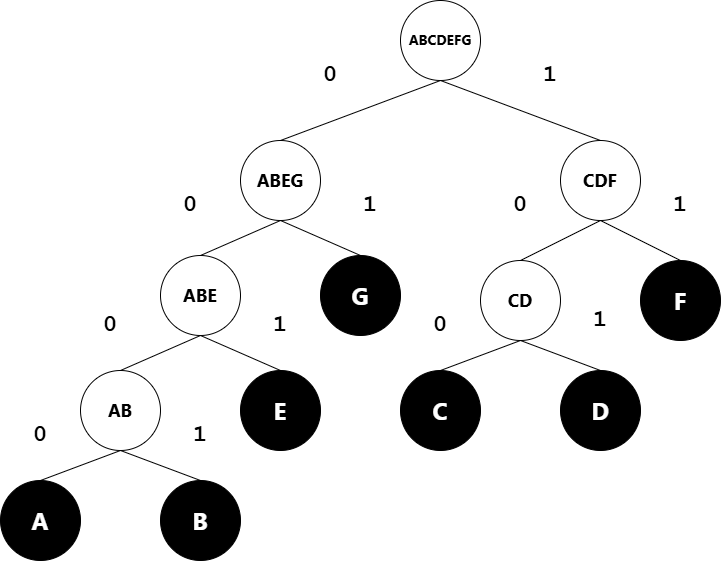
\includegraphics[width=9.5cm]{../images/hw7-1-1.png}
\caption{A Huffman tree for the given list of symbols and their frequencies, constructed using Huffman's algorithm.}
\label{fig:hw7_1_1}
\end{figure}

\begin{solution}
We can step through the recursive levels of Huffman's algorithm to construct a Huffman tree and obtain an optimal prefix code.

\textit{First. }The two lowest-frequency symbols are A and B with $f_{\rm A}=0.06$ and $f_{\rm B}=0.09$, respectively. We replace them with the pseudo-symbol AB such that $f_{\rm AB}=0.06+0.09=0.15$.

\textit{Second. }The two lowest-frequency symbols are C and D with $f_{\rm C}=0.10$ and $f_{\rm D}=0.12$, respectively. We replace them with the pseudo-symbol CD such that $f_{\rm CD}=0.10+0.12=0.22$.

\textit{Third. }The two lowest-frequency symbols are AB and E with $f_{\rm AB}=f_{\rm E}=0.15$. We replace them with the pseudo-symbol ABE such that $f_{\rm ABE}=0.15+0.15=0.30$.

\textit{Fourth. }The two lowest-frequency symbols are F and CD with $f_{\rm F}=0.16$ and $f_{\rm CD}=0.22$. We replace them with the pseudo-symbol CDF such that $f_{\rm CDF}=0.16+0.22=0.38$.

\textit{Fifth. }The two lowest-frequency symbols are ABE and G with $f_{\rm ABE}=0.30$ and $f_{\rm G}=0.32$. We replace them with the pseudo-symbol ABEG such that $f_{\rm ABEG}=0.30+0.32=0.62$.

\textit{Sixth. }The two remaining symbols are ABEG and CDF. We construct parent vertex ABCDEFG and take ABEG and CDF to be children of ABCDEFG.

Then, we reconstruct the tree by unwinding the recursion and re-attaching the terminal symbols, taking the psuedo-symbols to be their parent vertices. Finally, we can arbitrarily assign all left edges to represent a $0$ bit and all right edges to represent a $1$ bit. See Figure~\ref{fig:hw7_1_1}.

We can now construct the optimal prefix code for each symbol by traversing the tree from root to leaf and taking note of the edges followed:

\begin{center}
\begin{tabular}{c|c}
Letter&Encoding\\
A&0000\\
B&0001\\
C&100\\
D&111\\
E&001\\
F&11\\
G&01\\
\end{tabular}
\end{center}
This completes our encoding.
\end{solution}
\newpage
\item In general, are Huffman codes unique? That is, for a given set of letters and corresponding frequencies is there a unique Huffman encoding? Note that different letters may have the same frequency in the general case. If yes, justify. Otherwise provide a counterexample.
\begin{solution}
No, in general, Huffman codes are not unique.

First, bits are assigned to edges arbitrarily. For a given parent vertex, it is possible to let its left edge represent the $0$ bit and the right edge represent the $1$ bit, or to let the right represent $1$ and the left represent $0$. The only constraint on the assignment of bits is that one side must represent $0$ and the other must represent $1$. 

Furthermore, we can show that Huffman codes are not unique even with a consistent constraint on the assignment of the bits. 

Without loss of generality, assume that for every parent vertex, we always let its left child represent the $0$ bit and the right child represent the $1$ bit.

Consider four A, B, and C, with frequencies $f_{\rm A}=f_{\rm B}=f_{\rm C}=0.\overline{3}$. We want to construct an optimal prefix code using Huffman's algorithm. On the first recursive level, we may choose any of A and B, B and C, or C and A to be the two lowest-frequency symbols. Consider two of these cases:
\begin{itemize}
\item Suppose we take A and B to be the two lowest-frequency symbols. Then we replace them with parent AB with frequency $f_{\rm AB}=0.\overline{6}$, with A as the left child and B as the right. Now AB and C are joined to a parent to construct the tree, with AB as the left child and C as the right. In our optimal Huffman code, we represent A with $01$, B with $00$, and C with $1$.

\item Suppose we take B and C to be the two lowest-frequency symbols. Then we replace them with parent BC with frequency $f_{\rm BC}=0.\overline{6}$, with C as the left child and b as the right. Now A and BC are joined to a parent to construct the tree, with A as the left child and C as the right. In our optimal Huffman code, we represent A with $0$, B with $10$ and C with $11$.
\end{itemize}
We have shown that with the same list of symbols and frequencies, Huffman's algorithm may produce entirely different optimal prefix codes. Thus, Huffman codes are not unique.
\end{solution}
\end{enumerate}
\newpage
\subsection{Minimizing number of colors}
Let $X$ be a set of $n$ intervals $[s_i, f_i)$ on the real line. A {\em proper coloring} of $X$ assigns a color to each interval so that overlapping intervals are always assigned different colors.  In this problem, we want to find a proper coloring of $X$ using a minimum possible number of colors. Let us call this (unknown) number $c^*$.
\begin{enumerate}
\item Given a problem instance $\{[s_i,f_i)\}$ and any point on the real line $t$, let $n_t$ denote the number of sets that contain $t$. Also, let $c = \max_t n_t$ (easy to see the maximum is well defined). Argue that $c^*\ge c$.
\begin{solution}
\textit{Claim. }Let $X$ be a set of $n$ intervals $[s_i,f_i)$ for $1\leq i\leq n$. For all $t\in\mathbb{R}$, let $n_t$ denote the number of intervals in $X$ that contain $t$. Let $c=\underset{t\in\mathbb{R}}{\max}(n_t)$. Let $c^*$ be the minimum number of colors required to produce a proper of coloring of $X$. Then $c^*\geq c$.

\textit{Proof. }Since there exists $c=\underset{t\in\mathbb{R}}{\max}(n_t)$, there exists $t^*\in\mathbb{R}$ where $c=n_{t^*}$.

By definition, there are $n_{t^*}$ intervals that contain the point $t^*$. So, $n_{t^*}$ intervals overlap at the point $t^*$. In a proper coloring of $X$, each of these $n_{t^*}$ overlapping intervals is assigned a unique color. This implies that there are at least $n_{t^*}$ colors in a proper coloring of $X$. Since $c^*$ is the minimum number of colors required to produce a proper coloring of $X$, we know $c^*\geq n_{t^*}$.

Of course, $c=n_{t^*}$. Ergo $c^*\geq c.~\square$
\end{solution}
\item Consider the following greedy algorithm for solving this problem.
    \vspace*{-1ex}
    \begin{code}
    \> Sort the intervals according to $s_i$. \\
    \> Initialize the current number $z$ of defined colors to $0$. \\
    \> \For $i = 1$ to $n$, perform the following greedy step. \\
    \> \> \If next interval $a_i = [s_i, f_i)$ cannot be legally colored
    with any color $1\le j\le z$\\
    \> \> \Then increment $z$ by $1$ and assign $a_i$ the new color $z$.\\
    \> \> \Else color $a_i$ with the smallest ``legal'' color
    $j\in \{1, \ldots, z\}$  \\
    \end{code}

Argue that the greedy algorithm above computes a valid coloring, and yet {\em never uses more than $c$ colors}, where $c$ is the quantity from part (a).%\hint{Assume the intervals to be sorted according to $s_i$ and prove the statement using induction.}
\begin{solution}

\end{solution}
\item What is the running time of this algorithm as a function of $n$ and $c^*$?
\begin{solution}   INSERT YOUR SOLUTION HERE   \end{solution}


\end{enumerate}
%  \lhead{\textbf{Basic Algorithms, Fall 2024 \\ CSCI-UA.0310-001}}
\chead{\Large{\textbf{Homework 8}}}
\def\lc{\left\lceil}   
\def\rc{\right\rceil}
\rhead{\textbf{Instructor: Rotem Oshman \\Name: Ishan Pranav}}
\runningheadrule
\firstpageheadrule
\cfoot{}
\stepcounter{subsection}
\subsection*{References}
Peer-reviewed with Crystal Huang.

\subsection{Breadth-first search}
Recall the {\sc BFS} algorithm from the lecture that runs on graph $G$ starting from root node $s \in V$:
\begin{code}
    {\sc BFS}$(G,s)$\\
    1 \> $s.color = gray$, $s.dist = 0$. \\
    2 \> \For $u \in V \setminus \{s\}$ \\
    3 \> \> $u.color = white$, $u.dist = \infty$ \\
    4 \> $Q = \emptyset$ \\
    5 \> $Q.enqueue(s)$ \\
    6 \> \While $Q \neq \emptyset$ \\
    7 \> \> $u = Q.dequeue()$ \\
    8 \> \> \For $v \in Adj[u]$ \\
    9 \> \> \> \If $v.color = white$ \\
    10 \> \> \> \> $v.color = gray$ \\
    11 \> \> \> \> $v.dist = u.dist+1$ \\
    12 \> \> \> \> $Q.enqueue(v)$ \\
    13 \> \> $u.color = black$
\end{code}
\newpage
\begin{enumerate}
    \item Consider the undirected graph shown in Figure~\ref{fig:box}.
    If we begin a BFS traversal starting at node $A$, in what order are the nodes visited? Assume that the adjacency list is ordered alphabetically, i.e., we visit earlier letters alphabetically first, so from $A$ we will visit $B$ before $C$, and so on.
    
    \begin{figure}[h]
        \centering
        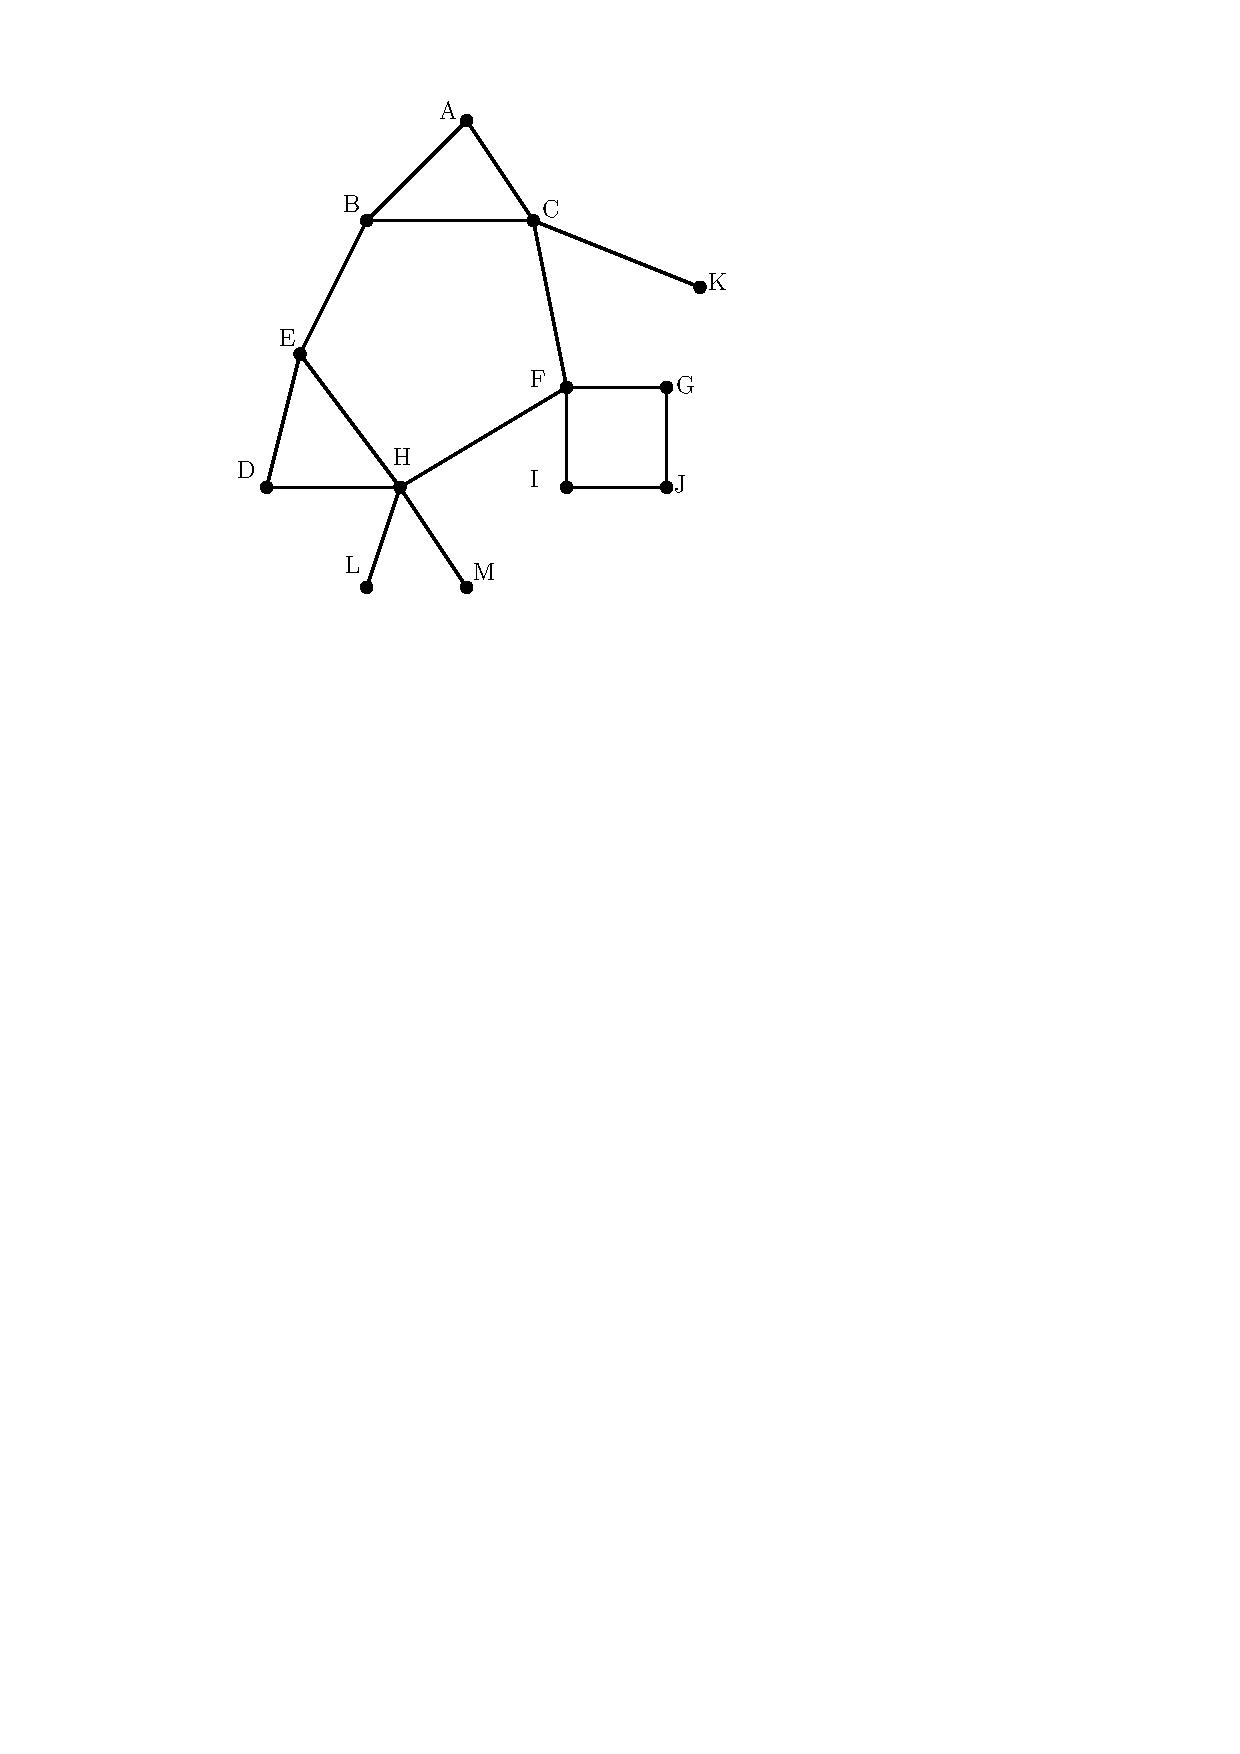
\includegraphics[width=0.4\textwidth]{images/BFS.pdf}
        \caption{Graph to traverse}
        \label{fig:box}
    \end{figure}
\begin{solution}
We can step through the breadth-first search algorithm to determine that the order of the vertices visited is A, B, C, E, F, K, D, H, G, I, L, M, and J.

\textit{First. }We enqueue A.

\textit{Second. }We dequeue A and enqueue B and C.

\textit{Third. }We dequeue B and enqueue E.

\textit{Fourth. }We dequeue C and enqueue F and K.

\textit{Fifth. }We dequeue E and enqueue D and H.

\textit{Sixth. }We dequeue F. We skip H. We enqueue G and I.

\textit{Seventh. }We dequeue K.

\textit{Eighth. }We dequeue H and enqueue L and M.

\textit{Ninth. }We dequeue G and enqueue J.

\textit{Tenth. }We dequeue I. We skip J.

\textit{Eleventh, twelfth, and thirteenth. }We dequeue L, M, and J.

The vertices are visited as enqueued: A, B, C, E, F, K, D, H, G, I, L, M, and J.
\end{solution}
\newpage
\item Explain what happens if we don't check whether a node is white before enqueuing it.
\begin{solution}
Suppose we did not check whether a node is white before enqueuing. Then the breadth-first search algorithm may not terminate.

For example, suppose we perform this variant of breadth-first search on graph $G=(V,E)$ with vertices $V=\{{\rm A},{\rm B},{\rm C}\}$ and edges $E=\{\{{\rm A},{\rm B}\}\}$. Assume, without loss of generality, that the initial vertex is A and that other vertices are visited in alphabetical order.

We can step through the algorithm to demonstrate the flaw.

\textit{First. }We enqueue A.

\textit{Second. }We dequeue A and enqueue B.

\textit{Third. }We dequeue B and enqueue A. Note that we enqueued A in this situation because we did not check its color and thus ignored the fact that it had been previously visited. 

This brings us back to the second step (dequeue A and enqueue B), meaning that the algorithm never terminates, even after all vertices have been visited.
\end{solution}
\newpage
\item Assume we replace the (FIFO) queue with a stack and therefore in line 7 obtain the node \emph{last} added. Does $v.dist$ still represent the shortest distance from $s$ to $v$?
\begin{solution}
No, using this implementation of breadth-first search, the distance assigned to a vertex $v$ may not represent the shortest distance from the starting vertex $s$ to $v$.

Consider the undirected graph $G=(V,E)$ with vertices $V=\{{\rm A},{\rm B},{\rm C},{\rm D},{\rm E}\}$ and edges $E=\{\{{\rm A},{\rm B}\},\{{\rm A},{\rm C}\},\{{\rm B},{\rm E}\},\{{\rm C},{\rm D}\},\{{\rm D},{\rm E}\}\}$. 

Assume, without los of generality, that the initial vertex is A and that other vertices are visited in alphabetical order.

We can see that the shortest path from A to E is $({\rm A},{\rm B},{\rm E})$, so the shortest distance from A to E is $2$.

However, if we step through the modified breadth-first search algorithm (a hybrid of breadth-first search and depth first search), we see that the algorithm handles the immediate children of the source node correctly, but mishandles its other descendent vertices.

\textit{First. }We push A with distance $0$.

\textit{Second. }We pop A, noting edges $\{{\rm A},{\rm B}\}$ and $\{{\rm A},{\rm C}\}$. We push B with distance $0+1=1$ and C with distance $0+1=1$.

\textit{Third. }We pop C, noting edge $\{{\rm C},{\rm D}\}$. We push D with distance $1+1=2$.

\textit{Fourth. }We pop D, noting edge $\{{\rm D},{\rm E}\}$. We push E with distance $2+1=3$. Already, this result is incorrect. We can continue stepping through the algorithm to show that it remains incorrect at termination.

\textit{Fifth. }We pop E.

\textit{Sixth. }We pop B, noting edge $\{{\rm B},{\rm E}\}$. We skip E.

The algorithm incorrectly assigns a distance of $3$ to E, although the shortest distance from A to E is $2$. We conclude that, in the modified algorithm, the distance assigned to $v$ is not necessarily the shortest distance from $s$ to $v$.
\end{solution}
\newpage
\item Consider graphs for which edges have assigned weights. Assume we modify line 11 of BFS to add the weight of the edge from $u$ to $v$ instead of adding $1$. Does the modified algorithm compute the shortest weighted distance correctly? If so, prove the correctness; otherwise, provide a counterexample for which the algorithm fails.
\begin{solution}
No, the modified algorithm is incorrect.

For example, suppose we perform this variant of the algorithm on graph $G=(V,E)$ with vertices $V=\{{\rm A},{\rm B},{\rm C},{\rm D}\}$ and edges $E$. For each edge $e\in E$, note $e=(u,v,w)$, where $u$ is the source vertex, $v$ is the target vertex, and $w$ is the weight of the edge. Suppose \[E=\{({\rm A},{\rm B},10),({\rm A},{\rm C},1),({\rm B},{\rm D},20),({\rm C},{\rm D},2)\}.\] Assume, without loss of generality, that $G$ is directed, that the initial vertex is A, and that other vertices are visited in alphabetical order.

We can step through the algorithm to demonstrate the flaw.

\textit{First. }We enqueue A with distance $0$.

\textit{Second. }We dequeue A, noting edges $({\rm A},{\rm B},10)$ and $({\rm A},{\rm C},20)$. We enqueue B with distance $0+10=10$ and C with distance $0+1=1$.

\textit{Third. }We dequeue B, noting edge $({\rm B},{\rm D},20)$. We enqueue D with distance $10+20=30$.

\textit{Fourth. }We dequeue C, noting edge $({\rm C},{\rm D},2)$. We skip D.

This gives $30$ for the distance from A to D by following path $({\rm A},{\rm B},{\rm D})$. However, there exists a path $({\rm A},{\rm C},{\rm D})$ whereby the distance from A to D is $3$. Of course, $3<30$. Thus, the modified algorithm fails.
\end{solution}
\end{enumerate}
\newpage
\subsection{Universal sink}
Recall that the \emph{adjacency matrix} representation of a \emph{directed} graph $G=(V,E)$ is the $|V| \times |V|$ matrix $M_G$ where $M_G[i][j]$ is $1$ if there is an edge from vertex $i$ to vertex $j$, and $0$ otherwise.
You may assume no vertex in the graph has an edge going into itself (i.e., no self-loops). We want to determine whether there is any vertex in $G$ that has edges coming to it from \emph{all other} vertices but no edges going out from it (this is known as a \textbf{universal sink}). 

\begin{enumerate}
\item Write an $O(|V|^2)$ algorithm that, given $M_G$, checks if there is a universal sink.
\begin{solution}

\textbf{Algorithm I. }{\sc IsSink}($M_G,v$) with a $|V|\times|V|$ adjacency matrix $M_G$ representing directed graph $G=(V,E)$ with no self-loops and a vertex $v\in V$; returns \verb|true| if $v$ is a universal sink; otherwise, \verb|false|:

For $u\in(V\setminus\{v\})$, if $M_G[v,u]=1$ or $M_G[u,v]=0$, then return \verb|false|.

Return \verb|true|.

\textbf{Algorithm II. }{\sc QuadraticSink}($M_G$) with a $|V|\times|V|$ adjacency matrix $M_G$ representing directed graph $G=(V,E)$ with no self-loops; returns \verb|true| if there is a universal sink in $G$; otherwise, \verb|false|:

For $v\in V$, if {\sc IsSink}($M_G,v$) is \verb|true|, then return \verb|true|.

Return \verb|false|.

\textbf{Proposition I. }\textit{Claim. }Algorithm I determines if $v$ is a universal sink in $G$ in running time $O(|V|)$.

\textit{Proof. }By definition, $v$ is a universal sink in $G=(V,E)$ if, for all $u\in V$ where $u\neq v$, we have $(u,v)\in E$ but $(v,u)\notin E$. The {\sc IsSink} algorithm compares $v$ to all other vertices $u$. It returns \verb|true| only if $v$ has edges coming to it from all other vertices $u$ and no edge going out from it to any vertex $u$. Otherwise, {\sc IsSink} returns \verb|false|. Thus, Algorithm I correctly determines if $v$ is a universal sink.

This implementation of Algorithm I visits every element in $V$ and performs constant-time operations within the loop body, so it has running time $O(|V|\times 1)=O(|V|).~\square$

\textbf{Proposition II. }\textit{Claim. }Algorithm II determines if there exists a universal sink in $G$ in running time $O(|V|^2)$.

\textit{Proof. }For $G=(V,E)$, The {\sc QuadraticSink} algorithm checks every vertex $v\in V$, using Algorithm I to determine if $v$ is a universal sink. From Proposition I, Algorithm I correctly determines if $v$ is a universal sink. Since Algorithm II returns \verb|true| if Algorithm I determines that any vertex is a universal sink (and \verb|false| if none satisfies this test), Algorithm II correctly determines if there exists a universal sink in $G$.

This implementation of Algorithm II visits every element in $V$ and performs {\sc IsSink} on each ($O(|V|)$ by Proposition I) within the loop body, so it has running time $O(|V|\times |V|)=O(|V|^2).~\square$
\end{solution}
\newpage
\item Write an $O(|V|)$ algorithm for the problem. Justify why it is correct, as well as why it satisfies this run-time bound.
\begin{solution}

\textbf{Algorithm III. }{\sc LinearSink}($M_G$) with a $|V|\times |V|$ adjacency matrix $M_G$ representing directed graph $G=(V,E)$ with no self-loops; returns \verb|true| if there is a universal sink in $G$; otherwise, \verb|false|:

If $V=\emptyset$, then return \verb|false|.

Let $v^*\leftarrow v\in V$, choosing $v$ arbitrarily.

Let $U\leftarrow V\setminus\{v^*\}$.

Let $W\leftarrow\emptyset$.

For $u\in U$:
\begin{itemize}
\item if $M_G[v^*][u]=1$ then:
\begin{itemize}
    \item assign $W\leftarrow W\cup\{v^*\}$;
    \item assign $v^*\leftarrow u$;
\end{itemize}
\item otherwise:
\begin{itemize}
    \item assign $W\leftarrow W\cup\{u\}$.
\end{itemize}
\end{itemize}

Return {\sc IsSink}($M_G,v^*$).

\textbf{Invariant I. }\textit{Claim. }For every step of the loop, no vertex $w\in W$ is a universal sink.

\textit{Proof. }We can prove this invariant by structural induction on $W$.

\textit{Basis. }Consider $W=\emptyset$. Then the invariant holds vacuously at initialization.

\textit{Hypothesis. }Consider $W=X$ where $X\neq\emptyset$. Assume there exists no universal sink $w\in W$.

\textit{Inductive step. }Consider $W=X\cup\{v\}$ for $v\in V$. From Algorithm III, there are two cases:
\begin{itemize}
\item Suppose $M_G[v^*][u]=1$. Then $v=v^*$ (before the reassignment of $v^*$). Thus $M_G[v][u]=1$, indicating that there is an outgoing edge from $v$, or $(v,u)\in E$. So $v$ is not a universal sink.
\item Suppose instead $M_G[v^*][u]=0$. Then $v=u$. Thus $M_G[v^*][v]=0$, indicating that there is no incoming edge to $v$, or $(v^*,v)\notin E$. So $v$ is not a universal sink.
\end{itemize}
In all cases, $v$ is not a universal sink.

For all $x\in X$, the invariant holds by the inductive hypothesis. Since the invariant holds for $v$, it must therefore hold for all vertices $w\in(X\cup\{v\})$.

Hence, by structural induction, there exists no universal sink $w\in W$. This invariant holds at initialization, maintenance, and termination.

\textbf{Proposition III. }\textit{Claim. }Algorithm III determines if there exists a universal sink in $G$ in running time $O(|V|)$.

\textit{Proof. }Suppose $V=\emptyset$. Then there is no universal sink in $G$, and Algorithm III returns \verb|false|, which is correct.

Suppose instead $V\neq\emptyset$. Then there exists an arbitrary $v^*\in V$. 

The loop executes for each of the $(|V|-1)$ elements in $U=V\setminus\{v^*\}$.

From Algorithm III, at initialization we have $|W|=0$. Also, for each iteration, exactly one element is inserted into $W$ in all cases. This implies that $|W|=(|V|-1)$ at termination. From Invariant I, at termination, we have for all $w\in W$ that $w$ is not a universal sink. Of course $v^*\notin W$, but $v^*\in V$. In fact, $v^*$ is the only vertex that has not been eliminated.

If $v^*$ is a universal sink, then there is a universal sink in $G$; otherwise, there is none.

Algorithm III returns $\textsc{IsSink}(M_G,v^*)$, which, by Proposition I, correctly determines if $v^*$ is a universal sink. Thus, Algorithm III correctly determines if there exists a universal sink in $G$.

The loop body performs constant-time operations in all cases, so the running time of the loop is $O((|V|-1)\times 1)=O(|V|-1)$. The running time of $\textsc{IsSink}(M_G,v^*)$ is $O(|V|)$ from Proposition I. Thus, the running time of \sc{LinearSink} is $O(|V|-1)+O(|V|)=O(|V|).~\square$
\end{solution}
\end{enumerate}

  %\lhead{\textbf{Basic Algorithms, Fall 2024 \\ CSCI-UA.0310-001}}
\chead{\Large{\textbf{Homework 9}}}
\def\lc{\left\lceil}   
\def\rc{\right\rceil}
\rhead{\textbf{Instructor: Rotem Oshman \\ Name: Ishan Pranav}}
\runningheadrule
\firstpageheadrule
\cfoot{}
\stepcounter{subsection}
\subsection*{References}
Collaborated with Crystal Huang.
\subsection{Sum of degrees}
Prove that in any undirected graph, 
the sum of the degrees of all the vertices is an even number. Recall that the degree of each vertex is the number of edges that include it. For example, in Figure~\ref{fig:box} node $B$ has degree $3$ and node $D$ has degree $2$.

\begin{figure}[htb]
    \centering
    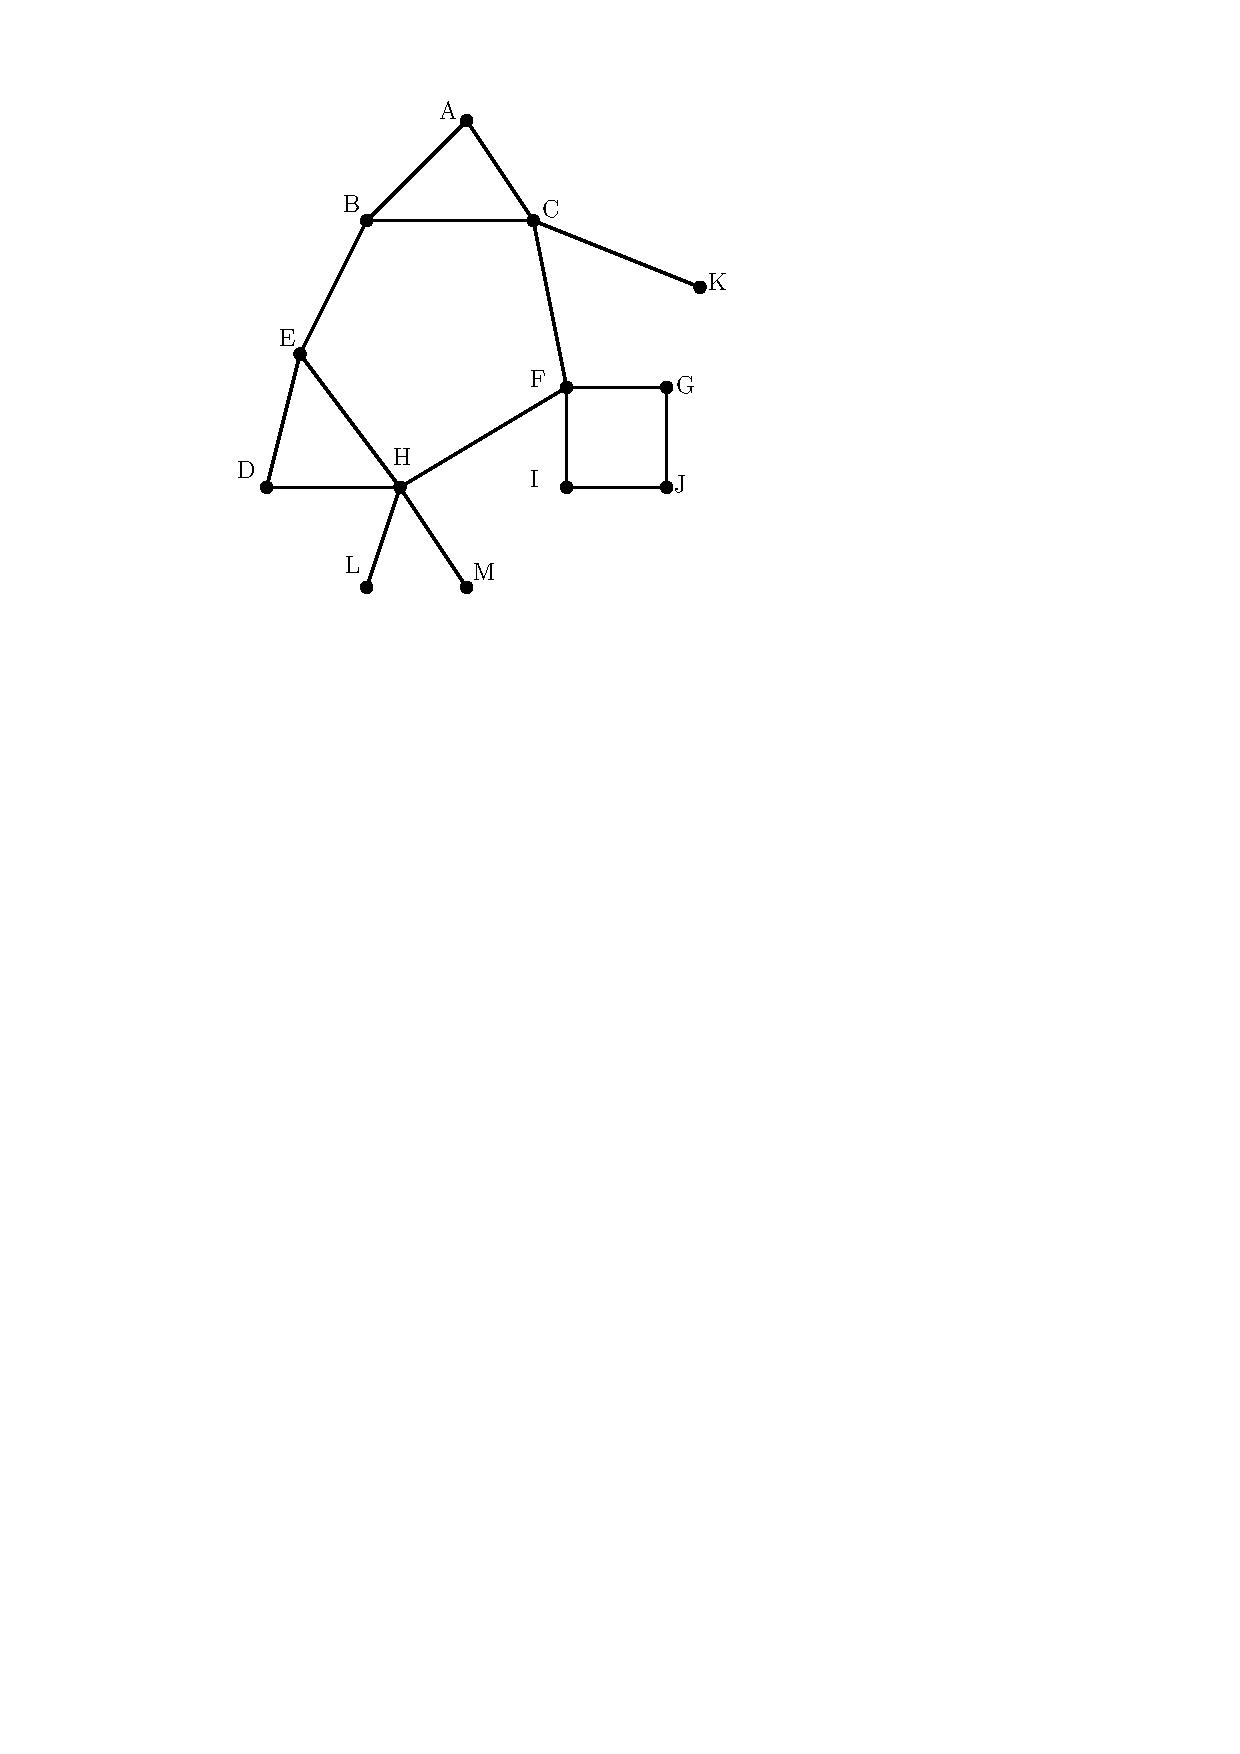
\includegraphics[width=0.4\textwidth]{images/BFS.pdf}
    \caption{An example graph}
    \label{fig:box}
\end{figure}
\begin{solution}
\textit{Claim. }Let $G=(V,E)$ be an undirected graph. Then there exists $k\in\mathbb{Z}$ such that \[\sum_{v\in V}{d_G(v)}=2k,\] where $d(v)$ denotes the degree of vertex $v\in V$ in graph $G$.\\

\noindent\textit{Proof. }We can demonstrate the claim by structural induction on $G$.\\

\noindent\textit{Basis. }Consider $G=(V,\emptyset)$. Then there are no edges in $G$, so for all $v\in V$, we have $d_G(v)=0$. Thus \[\sum_{v\in V}{d_G(v)}=\sum_{v\in V}0=0=2\cdot 0,\]
so the claim holds in the base case.\\

\noindent\textit{Hypothesis. }Consider $G=H=(V,E)$ where $E\neq\emptyset$. Assume that the sum of the degrees of all vertices in graph $H$ is even.\\

\noindent\textit{Inductive step. }Consider $G=(V,E\cup\{\{u,v\}\})$ where $u,v\in V$ and $\{u,v\}\notin E$. Observe
\begin{align*}
\sum_{w\in V}{d_H(w)}
&=d_H(u)+d_H(v)+\sum_{w\in V\setminus\{u,v\}}(d_H(w))\\
&=d_H(u)+d_H(v)+\sum_{w\in V\setminus\{u,v\}}(d_G(w))&\textit{since no $w\in V\setminus\{u,v\}$ is in the new edge,}\\
&=(d_G(u)+1)+(d_G(v)+1)+\sum_{w\in V\setminus\{u,v\}}(d_G(w))&\textit{since $u,v\in\{u,v\}$ but $\{u,v\}\notin E$,}\\
&=2+d_G(u)+d_G(v)+\sum_{w\in V\setminus\{u,v\}}(d_G(w))\\
&=2+\sum_{w\in V}(d_G(w))\\
&=2+2k&\textit{by the inductive hypothesis}\\
&=2(k+1)&\textit{thus completing the inductive step.}
\end{align*}
\noindent Hence, by structural induction, the sum of the degrees of all vertices in an undirected graph is even.$~\square$
\end{solution}
\newpage
\subsection{DFS (5+5+5=15 points)}

\begin{enumerate}
\item 
Consider the graph in Figure~\ref{fig:box2}. Say we begin a DFS traversal starting at node $A$. List the discovery (i.e., when we mark a node ``gray'') and finishing times (i.e., when we mark a node ``black'') of all the vertices (you may assume each successive step in the traversal takes time 1). Assume that the adjacency lists in the representation of the input graph are in alphabetical order.
\begin{figure}[h!]
\centering
    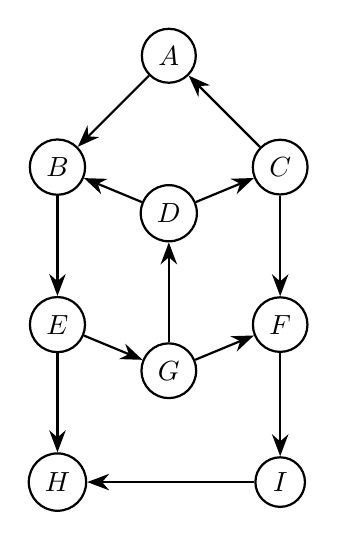
\begin{tikzpicture}[node distance={20mm}, thick,main/.style={circle, thick,draw,font=\sffamily\bfseries}, ar/.style={-{Stealth[scale=1.2]}}]
          \node[main] (1) {$A$}; 
          \node[main] (2) [below left of=1]{$B$};
          \node[main] (3) [below right of=1]{$C$};
          \node[main] (4) [below of=1]{$D$};
          \node[main] (5) [below left of=4]{$E$};
          \node[main] (6) [below right of=4]{$F$};
          \node[main] (7) [below of=4]{$G$};
          \node[main] (8) [below left of=7]{$H$};
          \node[main] (9) [below right of=7]{$I$};
          
          \draw[ar] (1) -- (2);
          \draw[ar] (3) -- (1);
          \draw[ar] (4) -- (3);
          \draw[ar] (2) -- (5);
          \draw[ar] (7) -- (4);
          \draw[ar] (5) -- (7);
          \draw[ar] (5) -- (8);
          \draw[ar] (9) -- (8);
          \draw[ar] (6) -- (9);
          \draw[ar] (3) -- (6);
          \draw[ar] (4) -- (2);
          \draw[ar] (7) -- (6);
          
    \end{tikzpicture}
    \caption{Graph for Question 4.1}
          \label{fig:box2}
\centering
\end{figure}

    \begin{center}
    \begin{tabular}{|c|c|c|c|c|c|c|c|c|c|}
    \hline
         Node & A & B & C & D & E & F & G & H & I\\
         \hline 
         $d$-time &  &  &  &  &  &  &  &  & \\
         \hline
         $f$-time &  &  &  &  &  &  &  &  &  \\
         \hline
    \end{tabular}
    \end{center}


\begin{solution}   INSERT YOUR SOLUTION HERE   \end{solution}
\end{enumerate}    

\noindent
As in the previous question, for any vertex $a$ in directed graph $G$, we denote by $a.\mathsf{d} $ the time at which DFS on $G$ discovers (i.e., marks as ``gray'') the vertex $a$. Similarly, denote by $a.\mathsf{f} $ the time at which DFS fully explores (i.e., marks as ``black'') the vertex $a$. Give counterexamples to the following statements:
\begin{enumerate}[start=2]
    \item If a directed graph $G$ contains a path
    from $a$ to $b$, and if $a.\mathsf{d} < b.\mathsf{d}$ in a depth-first search of $G$, then $b$ is a descendant
    of $a$ in the depth-first forest produced.

\begin{solution}   INSERT YOUR SOLUTION HERE   \end{solution}
    \item If a directed graph $G$ contains a path
    from $a$ to $b$, then any depth-first search must result in $b.\mathsf{d} < a.\mathsf{f}$.
\begin{solution}   INSERT YOUR SOLUTION HERE   \end{solution}
\end{enumerate}


\subsection{2-Colorings (5+6+5=16 points)}
A \emph{2-coloring} of an undirected graph $G = (V,E)$ assigns each node $v \in V$ a color $v.color \in \{red,green\}$ such that $u.color \neq v.color$ for all $(u,v) \in E$. We say the graph $G$ is 
2-colorable if such a 2-coloring exists. (A simple example where no 2-coloring exists is a ``triangle'' graph, i.e., the fully connected graph with 3 vertices.)

\begin{enumerate}
    \item 
    Show that if $G$ is a tree (i.e., connected and acyclic), then there always exists a 2-coloring. How many different 2-colors exist for such a graph?

\begin{solution}   INSERT YOUR SOLUTION HERE   \end{solution}


	\item 
	Describe how to modify the algorithm for Depth First Search so that it assigns a valid 2-coloring, or returns an error in case none exists. To this end, write a function {\sc TwoColoring-Visit}$(G,u,c)$ that takes a graph $G$, a vertex $u$, and a color $c \in \{red,green\}$ such that the following driver function either assigns a valid 2-coloring and returns $success$, or returns $error$ in case no 2-coloring exists. Your algorithm should assume $G$ to be represented as an adjacency list and run in $O(|V| + |E|)$. 
	
	\begin{code}
		{\sc TwoColoring}$(G)$\\
		\> \For $u \in G.V$ \Do \\
		\> \> $u.color = white$ \\
		\> \For $u \in G.V$ \Do \\
		\> \> \If $u.color \stackrel{?}{=} white$ \Then \\
		\> \> \> $\text{\sc TwoColoring-Visit}(G,u,red)$ \\
		\> \Return $success$ \\
	\end{code}

\begin{solution}   INSERT YOUR SOLUTION HERE   \end{solution}

    \item Prove the correctness of your algorithm. More concretely, show (a) that the assigned coloring is always a valid 2-coloring, and (b) if a 2-coloring exists then the algorithm does assign one.
    \hint{Consider the DFS tree and the edge classification. You may reuse ideas from the first subproblem.}
    
\begin{solution}   INSERT YOUR SOLUTION HERE   \end{solution}
\end{enumerate}

  %\lhead{\textbf{Basic Algorithms, Fall 2024 \\ CSCI-UA.0310-001}}
\chead{\Large{\textbf{Homework 10}}}
\def\lc{\left\lceil}   
\def\rc{\right\rceil}
\newtheorem{claim}{Claim}
\newtheorem{property}{Property}
\rhead{\textbf{Instructor: Rotem Oshman \\Name: Ishan Pranav}}
\runningheadrule
\firstpageheadrule
\cfoot{}
\stepcounter{subsection}
\subsection*{References}
Peer-reviewed with Crystal Huang.
\subsection{Tours}
Suppose the New York Botanical Gardens are trying to drum up interest for their tree and shrub collections by offering tours through the arboretum, and you are tasked with reviewing their proposed routes. There are a set $V$ of trees they want some tour to stop at, and a set $E$ of routes from tree to tree their proposed tours would make. In order to make sure all the trees are visited, they want the following property:
\begin{property} 
For all pairs $v, u\in V$, we must have a path from $u$ to $v$ or a path from $v$ to $u$ (or both). 
\end{property}
\noindent They provide you with many proposed plans and a strict deadline for your feedback, and so you want to develop an efficient algorithm to automate this task. 

\begin{enumerate}
\item Suppose $G = (V, E)$ is a directed acyclic graph. Design a simple $O(|V|+|E|)$ time algorithm to determine whether or not the given graph $G$ satisfies the desired property. For example, in Figure~\ref{fig:q1-1}, the first example satisfies the property while the second does not (as there is no path from $A$ to $C$ nor from $C$ to $A$).
Argue the correctness of your algorithm.

\hint{Base your algorithm on topological sort.} 

\hint{\noindent
\begin{minipage}[t]{0.95\linewidth}
If we change the examples to
$A \leftarrow B \rightarrow C \rightarrow D$ and 
$B \rightarrow A \rightarrow C \rightarrow D$, then $(B,A,C,D)$ is a valid topological sort of both, but one of the graphs satisfies the property while the other one does not. Draw the edges of each graph on the vertices in topological order. What is the difference?
\end{minipage}}

\begin{figure}[htb]
    \centering
    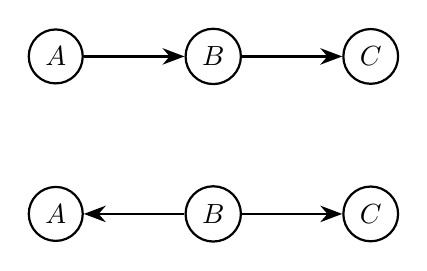
\begin{tikzpicture}[node distance={20mm}, thick,main/.style={circle, thick,draw,font=\sffamily\bfseries}, ar/.style={-{Stealth[scale=1.2]}}]
      \node[main] (1) {$A$}; 
      \node[main] (2) [right of=1]{$B$};
      \node[main] (3) [right of=2]{$C$};
      \node[main] (4) [below of=1]{$A$};
      \node[main] (5) [right of=4]{$B$};
      \node[main] (6) [right of=5]{$C$};
      
      \draw[ar] (1) -- (2);
      \draw[ar] (2) -- (3);
      \draw[ar] (5) -- (4);
      \draw[ar] (5) -- (6);
    \end{tikzpicture}
    \caption{Illustrations for Question 1-1.}
    \label{fig:q1-1}
\end{figure}


\begin{solution}   INSERT YOUR SOLUTION HERE   \end{solution}

\item Suppose now that $G = (V, E)$ is an arbitrary directed graph. Design a $O(|V|+|E|)$ time algorithm to determine whether or not the given graph $G$ satisfies the desired property. 

\hint{Recall that any directed graph $G$ can be decomposed into a DAG of strongly connected components. Can you reuse some ideas of your prior approach?}
\begin{solution}   INSERT YOUR SOLUTION HERE   \end{solution}


\item Prove that your algorithm in $(2)$ is correct and that it runs in the required time.
\begin{solution}   INSERT YOUR SOLUTION HERE   \end{solution}
\end{enumerate}


\subsection{Topological Sort (5+5=10 points)}
\begin{enumerate}
    \item How many valid topological sorts does the directed graph $G$ in Figure \ref{fig:topo-sort} below have? List all the valid topological sorts in the following table. One of them has been listed as an example, where node $A$ has the last finish time and $D$ has the first.

    \begin{figure}[H]
        \centering
        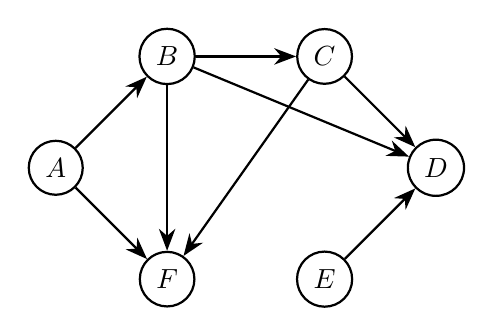
\begin{tikzpicture}[node distance={20mm}, thick,main/.style={circle, thick,draw,font=\sffamily\bfseries}, ar/.style={-{Stealth[scale=1.2]}}]
          \node[main] (1) {$A$}; 
          \node[main] (2) [above right of=1]{$B$};
          \node[main] (3) [right of=2]{$C$};
          \node[main] (4) [below right of=3]{$D$};
          \node[main] (5) [below right of=1]{$F$};
          \node[main] (6) [right of=5]{$E$};
          
          \draw[ar] (1) -- (2);
          \draw[ar] (1) -- (5);
          \draw[ar] (2) -- (3);
          \draw[ar] (2) -- (4);
          \draw[ar] (2) -- (5);
          \draw[ar] (3) -- (4);
          \draw[ar] (3) -- (5);
          \draw[ar] (6) -- (4);
        \end{tikzpicture}
        \caption{Directed $G$ for topological sort.}
        \label{fig:topo-sort}
    \end{figure}
    
     \begin{center}
    \begin{tabular}{c c c c c c c}
    \hline
     1. & A & B & C & F & E & D\\
     2. &  &  &  &  &  & \\
    \hline
    \end{tabular}
    \label{table:q3}
    \end{center}
\begin{solution}   INSERT YOUR SOLUTION HERE   \end{solution}
    

    \item 
    Give an example of a graph showing that the topological sort algorithm does not work if we output vertices in order of their discovery time, instead of reverse finish time.

\begin{solution}   INSERT YOUR SOLUTION HERE   \end{solution}
\end{enumerate}




\subsection{Spanning Tree (4+4+4=12 points)}

Recall that for an undirected graph $G = (V,E)$ as a spanning tree $T$ is a subgraph containing all vertices $V$ such that $T$ is connected and acyclic. 

In the following, let $e = (u,v) \in E$ be an edge that is \emph{not} part of $T$.
Prove the following properties:

\begin{enumerate}
    \item Assume we add $e$ to $T$, i.e., consider the graph $T'$ over the vertices $V$ that contains all edges from $T$ and $e$. Show that this graph is no longer acyclic.

\begin{solution}   INSERT YOUR SOLUTION HERE   \end{solution}

    \item Now let $e'$ be an arbitrary edge on the cycle created by adding $e$ to $T'$ in part (1). Let $T''$ be the graph obtained by removing $e'$, i.e., the graph obtained by replacing $e'$ with $e$ in the original spanning tree $T$. Show that $T''$ is connected.

\begin{solution}   INSERT YOUR SOLUTION HERE   \end{solution}

    \item Now complete the proof of $T''$ being a spanning tree by also showing that $T''$ is acyclic.

\begin{solution}   INSERT YOUR SOLUTION HERE   \end{solution}
\end{enumerate}
  %\lhead{\textbf{Basic Algorithms, Fall 2024 \\ CSCI-UA.0310-001}}
\chead{\Large{\textbf{Homework 11}}}
\def\lc{\left\lceil}   
\def\rc{\right\rceil}
\newtheorem{claim}{Claim}
\newtheorem{property}{Property}
\rhead{\textbf{Instructor: Rotem Oshman \\ Name: Ishan Pranav}}
\runningheadrule
\firstpageheadrule
\cfoot{}
\stepcounter{subsection}
\section*{References}
Collaborated with Crystal Huang.
\subsection{Prim and Kruskal}
\begin{figure}[h]
    \centering
    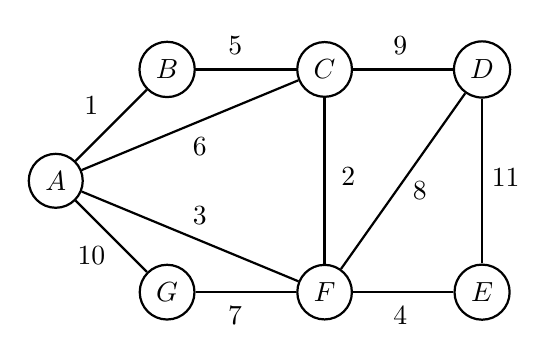
\begin{tikzpicture}[node distance={20mm}, thick,main/.style={circle, thick,draw,font=\sffamily\bfseries}, ar/.style={-{Stealth[scale=1.2]}}]
      \node[main] (1) {$A$}; 
      \node[main] (2) [above right of=1]{$B$};
      \node[main] (3) [right of=2]{$C$};
      \node[main] (4) [right of=3]{$D$};
      \node[main] (5) [below right of=1]{$G$};
      \node[main] (6) [right of=5]{$F$};
      \node[main] (7) [right of=6]{$E$};
      
      \draw (1) -- (2) node [at start, xshift=0.2cm, yshift=0.7cm]{$1$};
      \draw (1) -- (3) node [at start, xshift=1.5cm, yshift=0.3cm]{$6$};
      \draw (1) -- (5) node [at start, xshift=0.2cm, yshift=-0.7cm]{$10$};
      \draw (1) -- (6) node [at start, xshift=1.5cm, yshift=-0.3cm]{$3$};
      \draw (2) -- (3) node [at start, xshift=0.5cm, yshift=0.3cm]{$5$};
      \draw (3) -- (4) node [at start, xshift=0.6cm, yshift=0.3cm]{$9$};
      \draw (3) -- (6) node [at start, xshift=0.3cm, yshift=-1.0cm]{$2$};
      \draw (4) -- (7) node [at start, xshift=0.3cm, yshift=-1.0cm]{$11$};
      \draw (5) -- (6) node [at start, xshift=0.5cm, yshift=-0.3cm]{$7$};
      \draw (6) -- (7) node [at start, xshift=0.6cm, yshift=-0.3cm]{$4$};
      \draw (6) -- (4) node [at start, xshift=1.0cm, yshift=1.0cm]{$8$};
    \end{tikzpicture}
    \caption{\textbf{Undirected graph $\mathbf{G}$.}}
    \label{fig:mst}
\end{figure}

Consider the undirected weighted graph $G = (V, E)$ in Figure~\ref{fig:mst} above.
\begin{enumerate}
    \item  Illustrate a run of Kruskal's algorithm on this graph. State at each step which edge is added to the tree. We have filled the first step in for you. Here, we only want the edge added to the tree and not every edge that is considered. 
    
    \begin{center}
    \begin{tabular}{c|c|c|c|c|c|c|c}
         \textbf{Step} & 1 & 2 & 3 & 4 & 5 & 6\\
         \hline
         \textbf{Edge Added} & $AB$ &   &   &   &   & \\
    \end{tabular}
    \end{center}
\begin{solution}   INSERT YOUR SOLUTION HERE   \end{solution}
    \item Illustrate a run of Prim's algorithm on this graph starting from vertex $A$. State at each step which edge is added to the tree. We have filled the first step in for you. Here, we only want the edge added to the tree and not every edge that is considered. 
    
    \begin{center}
    \begin{tabular}{c|c|c|c|c|c|c|c}
         \textbf{Step} & 1 & 2 & 3 & 4 & 5 & 6\\
         \hline
         \textbf{Edge Added} & $AB$ &   &   &   &   &  \\
    \end{tabular}
    \end{center}
\begin{solution}   INSERT YOUR SOLUTION HERE   \end{solution}
\end{enumerate}


\subsection{Minimal spanning tree}
Prove or disprove the following statements. If true, give a short explanation. If false, give a counterexample.

\begin{enumerate}
\item Let $G = (V, E)$ be a connected, undirected graph with a distinct cost $c(e)$ on every edge $e$. Suppose $e^*$ is the cheapest edge in $G$; that is, $c(e^*) < c(e)$ for every edge $e \neq e^*$. Then there is a minimum spanning tree $T$ of $G$ that contains the edge $e^*$.
\begin{solution}

\textbf{Definition I. }Let $G=(V,E)$ be a connected, undirected graph with a distinct cost $c(e)$ for every edge $e\in E$.

\textbf{Definition II. }Let $e^*\in E$ be the cheapest edge in $G$; that is, we have $c(e^*)<c(e)$ for all $e\in E$ where $e\neq e^*$.

\textbf{Lemma I. }\textit{Claim. }Let $T=(V,E_T)$ be a spanning tree of $G$ where $e^*\notin T$. We can construct a spanning tree of $G$ whose total cost is less than that of $T$.

Since $T$ is a spanning tree of $G$, there exists a path $(u,\dots,x,y,\dots,v)$ in $T$ containing an edge $e'=\{x,y\}$ for $x,y\in V$. Of course, $e'\neq e^*$ since $T$ does not contain $e^*$.

We can add edge $e^*$ to $T$ to construct $T'=(V,E_T\cup\{e^*\})$, an induced subgraph of $G$. Now there exists a cycle $(u,\dots,x,y,\dots,v,u)$ in $T'$ that contains $e'$. Note that $T'$ is connected because $T$ is a tree, and thus connected.

We can construct $T''=(V,(E_T\cup\{e^*\})\setminus\{e'\})$, an induced subgraph of $G$ derived by replacing $e^*$ with $e'$ in $T$; that is, by removing $e'$ from $T'$.

After severing the edge $e'=\{x,y\}$, paths $(x,\dots,u)$ and $(v,\dots,y)$ still do exist in $T''$. Since edge $e=\{u,v\}$ does exist in $T''$, there exists a path $(x,\dots,u,v,\dots,y)$ in $T''$. All other vertices in $T''$ are connected because $T'$ is connected. So $T''$ is connected. 

Without $e'=\{x,y\}$, the cycle $(u,\dots,x,y,\dots,v,u)$ does not exist in $T''$. By construction, this is the only cycle in $T''$ since $T$ is a tree, and thus, acyclic. Thus, $T''$ is acyclic.

By construction of $T''$, the total cost of all edges in $T''$ is the total cost of all edges in $T$, minus the cost of $e'$, plus the cost of $e^*$. Since $c(e^*)$ is the cheapest edge in $G$, and $e'\in G$, we know $c(e^*)<c(e')$. Therefore, the total cost of all edges in $T''$ is less than that of all edges in $T$.

Since $T''$ is a connected, acyclic, induced subgraph of $G$ containing all vertices in $G$, we know that $T''$ is a spanning tree. $T''$ is a spanning tree of $G$ with a smaller total cost than $T$---what was to be constructed.

\textbf{Proposition I. }\textit{Claim. }There exists a minimum spanning tree of $G$ that contains $e^*$.

\textit{Proof. }Assume, for the sake of contradiction, that there exists no minimum spanning tree of $G$ that contains edge $e^*=\{u,v\}$ for $u,v\in V$. Let $T=(V,E_T)$ be a minimum spanning tree of $G$. It follows from our hypothesis that $e^*\notin E_T$.

From Lemma I, since $T$ is a spanning tree of $G$ that does not contain its cheapest edge $e^*$, we can construct a spanning tree of $G$ whose total cost is less than that of $T$.

This is absurd: It contradicts the hypothesis that $T$ is a \textit{minimum} spanning tree of $G$. Ergo, the hypothesis is false: There does exist a minimum spanning tree of $G$ containing $e^*.~\square$
\end{solution}
\newpage
\item In the above setting, every MST of $G$ contains the edge $e^*$.
\begin{solution}
\textbf{Proposition II. }\textit{Claim. }Every minimum spanning tree of $G$ contains $e^*$.

\textit{Proof. }Assume, for the sake of contradiction, that there exists some minimum spanning tree $T=(V,E_T)$ of $G$ where $e^*\notin E_T$.

From Lemma I, since $T$ is a spanning tree of $G$ that does not contain its cheapest edge $e^*$, we can construct a spanning tree of $G$ whose total cost is less than that of $T$.

This is absurd: It contradicts the hypothesis that $T$ is a \textit{minimum} spanning tree of $G$. Ergo, the hypothesis is false: Every minimum spanning tree of $G$ does contain $e^*.~\square$
\end{solution}
\newpage
\end{enumerate}
\subsection{Faster minimal spanning tree}
\begin{enumerate}
    \item Assume that all edge weights of the given undirected graph $G = (V, E)$ are promised to be $1$. Design the fastest algorithm you can to compute the minimum spanning tree (MST) of $G$. Argue the correctness of the algorithm and state its run-time. 
    
    \hint{It should be more efficient than the $O(|E| \log |V|)$ run-time of Prim and Kruskal.}
\begin{solution}

\textbf{Algorithm 1. }{\sc SpanningTree}($G$) with undirected graph $G=(V,E)$, returns a minimum spanning tree of $G$:

Let $T=(V,E_T)$ with $E_T\leftarrow\emptyset$.

If $V=\emptyset$, then return $T$.

Let $s\leftarrow v\in V$, choosing $s$ arbitrarily.

Perform {\sc DepthFirstSearch}($s,G$); here {\sc DepthFirstSearch} is the well-known depth-first-search algorithm that visits each vertex in a graph once beginning from a source $s\in V$ and assigning $u.\mathsf{parent}$ to some vertex $v\in V$ for each $u\in V\setminus\{s\}$. Note {\sc DepthFirstSearch} has running time $O(|V|+|E|)$.

For $v\in V\setminus\{s\}$, assign $E_T\leftarrow E_T\cup\{\{v.\mathsf{parent},v\}\}$, via adjacency list.

Return $T$.

\textbf{Proposition 1. }\textit{Claim. }{\sc SpanningTree}($G$) is correct.

\textit{Proof. }

\textbf{Proposition 2. }\textit{Claim. }{\sc SpanningTree}($G$) has running time $O(|V|+|E|)$.

\textit{Proof. }First, Algorithm 1 invokes {\sc DepthFirstSearch} with running time $O(|V|+|E|)$.

Then, for each of the $|V|-1$ vertices in $V\setminus\{s\}$, it inserts an edge into $T$ via adjacency list, an $O(1)$ operation. Thus, the running time of the loop is $O(|V|)$.

Finally, Algorithm 1 returns the resulting tree, an $O(1)$ operation.

Thus, the running time of {\sc SpanningTree}($G$) is $O(|V|+|E|)+O(|V|)=O(|V|+|E|).~\square$
\end{solution}
    \item Suppose instead that all edge weights are 1 \emph{except} for a single edge $e_0 = (u_0, v_0)$ whose weight is $w_0$ (note, $w_0$ might be either larger or smaller than 1). Show how to modify your solution in part 1 to compute the MST of $G$. What is the running time of your algorithm and how does it compare to the runtime you obtained in part 1 (or standard Prim)?
\begin{solution}   INSERT YOUR SOLUTION HERE   \end{solution}
\end{enumerate}
  %\lhead{\textbf{Basic Algorithms, Fall 2024 \\ CSCI-UA.0310-001}}
\chead{\Large{\textbf{Homework 12}}}
\def\lc{\left\lceil}   
\def\rc{\right\rceil}
\newtheorem{claim}{Claim}
\newtheorem{property}{Property}
\rhead{\textbf{Instructor: Rotem Oshman\\ Name: Ishan Pranav}}
\runningheadrule
\firstpageheadrule
\cfoot{}
\stepcounter{subsection}
\subsection*{References}
Collaborated with Crystal Huang.
\subsection{Dijkstra}
Show the running of Dijkstra's algorithm for finding the distance from $A$ to all other vertices in the following graph. You should show the updated distances to all the vertices (i.e., the key of the vertex in the priority queue) after each step in the algorithm.

\begin{figure}[h!]
\begin{center}
  \resizebox{!}{!}{  

\tikzset{every picture/.style={line width=0.75pt}} %set default line width to 0.75pt        

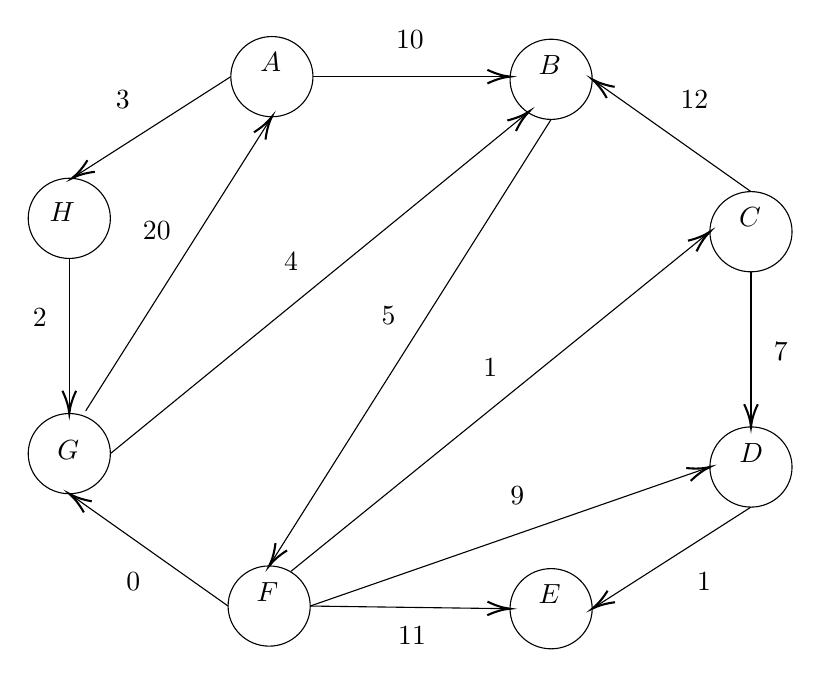
\begin{tikzpicture}[x=0.75pt,y=0.75pt,yscale=-1,xscale=1]
%uncomment if require: \path (0,443); %set diagram left start at 0, and has height of 443

%Shape: Ellipse [id:dp4366659013151436] 
\draw   (193.61,59.32) .. controls (193.61,48.65) and (202.46,40) .. (213.39,40) .. controls (224.32,40) and (233.18,48.65) .. (233.18,59.32) .. controls (233.18,70) and (224.32,78.65) .. (213.39,78.65) .. controls (202.46,78.65) and (193.61,70) .. (193.61,59.32) -- cycle ;
%Shape: Ellipse [id:dp1933565130763586] 
\draw   (328.14,60.61) .. controls (328.14,49.94) and (337,41.29) .. (347.93,41.29) .. controls (358.86,41.29) and (367.71,49.94) .. (367.71,60.61) .. controls (367.71,71.28) and (358.86,79.93) .. (347.93,79.93) .. controls (337,79.93) and (328.14,71.28) .. (328.14,60.61) -- cycle ;
%Shape: Ellipse [id:dp6804484495341399] 
\draw   (424.43,134.04) .. controls (424.43,123.37) and (433.29,114.72) .. (444.22,114.72) .. controls (455.14,114.72) and (464,123.37) .. (464,134.04) .. controls (464,144.71) and (455.14,153.36) .. (444.22,153.36) .. controls (433.29,153.36) and (424.43,144.71) .. (424.43,134.04) -- cycle ;
%Shape: Ellipse [id:dp5474703006205862] 
\draw   (424.43,247.4) .. controls (424.43,236.73) and (433.29,228.08) .. (444.22,228.08) .. controls (455.14,228.08) and (464,236.73) .. (464,247.4) .. controls (464,258.07) and (455.14,266.72) .. (444.22,266.72) .. controls (433.29,266.72) and (424.43,258.07) .. (424.43,247.4) -- cycle ;
%Shape: Ellipse [id:dp8638791225560539] 
\draw   (328.14,315.68) .. controls (328.14,305) and (337,296.35) .. (347.93,296.35) .. controls (358.86,296.35) and (367.71,305) .. (367.71,315.68) .. controls (367.71,326.35) and (358.86,335) .. (347.93,335) .. controls (337,335) and (328.14,326.35) .. (328.14,315.68) -- cycle ;
%Shape: Ellipse [id:dp008449392382588905] 
\draw   (192.29,314.39) .. controls (192.29,303.72) and (201.14,295.07) .. (212.07,295.07) .. controls (223,295.07) and (231.86,303.72) .. (231.86,314.39) .. controls (231.86,325.06) and (223,333.71) .. (212.07,333.71) .. controls (201.14,333.71) and (192.29,325.06) .. (192.29,314.39) -- cycle ;
%Shape: Ellipse [id:dp33826626675219873] 
\draw   (96,240.96) .. controls (96,230.29) and (104.86,221.64) .. (115.78,221.64) .. controls (126.71,221.64) and (135.57,230.29) .. (135.57,240.96) .. controls (135.57,251.63) and (126.71,260.28) .. (115.78,260.28) .. controls (104.86,260.28) and (96,251.63) .. (96,240.96) -- cycle ;
%Shape: Ellipse [id:dp6507975960123465] 
\draw   (96,127.6) .. controls (96,116.93) and (104.86,108.28) .. (115.78,108.28) .. controls (126.71,108.28) and (135.57,116.93) .. (135.57,127.6) .. controls (135.57,138.27) and (126.71,146.92) .. (115.78,146.92) .. controls (104.86,146.92) and (96,138.27) .. (96,127.6) -- cycle ;
%Straight Lines [id:da4219287944911677] 
\draw    (369.35,61.77) -- (444.22,114.72) ;
\draw [shift={(367.71,60.61)}, rotate = 35.27] [color={rgb, 255:red, 0; green, 0; blue, 0 }  ][line width=0.75]    (10.93,-3.29) .. controls (6.95,-1.4) and (3.31,-0.3) .. (0,0) .. controls (3.31,0.3) and (6.95,1.4) .. (10.93,3.29)   ;
%Straight Lines [id:da5980913207552611] 
\draw    (117.42,261.44) -- (192.29,314.39) ;
\draw [shift={(115.78,260.28)}, rotate = 35.27] [color={rgb, 255:red, 0; green, 0; blue, 0 }  ][line width=0.75]    (10.93,-3.29) .. controls (6.95,-1.4) and (3.31,-0.3) .. (0,0) .. controls (3.31,0.3) and (6.95,1.4) .. (10.93,3.29)   ;
%Straight Lines [id:da9818030529391072] 
\draw    (444.22,153.36) -- (444.22,226.08) ;
\draw [shift={(444.22,228.08)}, rotate = 270] [color={rgb, 255:red, 0; green, 0; blue, 0 }  ][line width=0.75]    (10.93,-3.29) .. controls (6.95,-1.4) and (3.31,-0.3) .. (0,0) .. controls (3.31,0.3) and (6.95,1.4) .. (10.93,3.29)   ;
%Straight Lines [id:da8226912095218192] 
\draw    (444.22,266.72) -- (369.4,314.6) ;
\draw [shift={(367.71,315.68)}, rotate = 327.39] [color={rgb, 255:red, 0; green, 0; blue, 0 }  ][line width=0.75]    (10.93,-3.29) .. controls (6.95,-1.4) and (3.31,-0.3) .. (0,0) .. controls (3.31,0.3) and (6.95,1.4) .. (10.93,3.29)   ;
%Straight Lines [id:da9411403626711399] 
\draw    (231.86,314.39) -- (326.14,315.65) ;
\draw [shift={(328.14,315.68)}, rotate = 180.77] [color={rgb, 255:red, 0; green, 0; blue, 0 }  ][line width=0.75]    (10.93,-3.29) .. controls (6.95,-1.4) and (3.31,-0.3) .. (0,0) .. controls (3.31,0.3) and (6.95,1.4) .. (10.93,3.29)   ;
%Straight Lines [id:da04931761460163331] 
\draw    (233.18,59.32) -- (326.14,59.32) ;
\draw [shift={(328.14,59.32)}, rotate = 180] [color={rgb, 255:red, 0; green, 0; blue, 0 }  ][line width=0.75]    (10.93,-3.29) .. controls (6.95,-1.4) and (3.31,-0.3) .. (0,0) .. controls (3.31,0.3) and (6.95,1.4) .. (10.93,3.29)   ;
%Straight Lines [id:da7139612650029891] 
\draw    (115.78,146.92) -- (115.78,219.64) ;
\draw [shift={(115.78,221.64)}, rotate = 270] [color={rgb, 255:red, 0; green, 0; blue, 0 }  ][line width=0.75]    (10.93,-3.29) .. controls (6.95,-1.4) and (3.31,-0.3) .. (0,0) .. controls (3.31,0.3) and (6.95,1.4) .. (10.93,3.29)   ;
%Straight Lines [id:da15021042776281257] 
\draw    (193.61,59.32) -- (118.79,107.2) ;
\draw [shift={(117.1,108.28)}, rotate = 327.39] [color={rgb, 255:red, 0; green, 0; blue, 0 }  ][line width=0.75]    (10.93,-3.29) .. controls (6.95,-1.4) and (3.31,-0.3) .. (0,0) .. controls (3.31,0.3) and (6.95,1.4) .. (10.93,3.29)   ;
%Straight Lines [id:da05554213731104107] 
\draw    (123.7,220.35) -- (212.32,80.34) ;
\draw [shift={(213.39,78.65)}, rotate = 122.33] [color={rgb, 255:red, 0; green, 0; blue, 0 }  ][line width=0.75]    (10.93,-3.29) .. controls (6.95,-1.4) and (3.31,-0.3) .. (0,0) .. controls (3.31,0.3) and (6.95,1.4) .. (10.93,3.29)   ;
%Straight Lines [id:da4376820533976681] 
\draw    (135.57,240.96) -- (335.83,77.34) ;
\draw [shift={(337.38,76.07)}, rotate = 140.75] [color={rgb, 255:red, 0; green, 0; blue, 0 }  ][line width=0.75]    (10.93,-3.29) .. controls (6.95,-1.4) and (3.31,-0.3) .. (0,0) .. controls (3.31,0.3) and (6.95,1.4) .. (10.93,3.29)   ;
%Straight Lines [id:da22701364215684228] 
\draw    (213.14,293.37) -- (347.93,79.93) ;
\draw [shift={(212.07,295.07)}, rotate = 302.27] [color={rgb, 255:red, 0; green, 0; blue, 0 }  ][line width=0.75]    (10.93,-3.29) .. controls (6.95,-1.4) and (3.31,-0.3) .. (0,0) .. controls (3.31,0.3) and (6.95,1.4) .. (10.93,3.29)   ;
%Straight Lines [id:da5780556586002948] 
\draw    (222.62,297.64) -- (422.88,135.3) ;
\draw [shift={(424.43,134.04)}, rotate = 140.97] [color={rgb, 255:red, 0; green, 0; blue, 0 }  ][line width=0.75]    (10.93,-3.29) .. controls (6.95,-1.4) and (3.31,-0.3) .. (0,0) .. controls (3.31,0.3) and (6.95,1.4) .. (10.93,3.29)   ;
%Straight Lines [id:da7820765166034285] 
\draw    (231.86,314.39) -- (422.54,248.06) ;
\draw [shift={(424.43,247.4)}, rotate = 160.82] [color={rgb, 255:red, 0; green, 0; blue, 0 }  ][line width=0.75]    (10.93,-3.29) .. controls (6.95,-1.4) and (3.31,-0.3) .. (0,0) .. controls (3.31,0.3) and (6.95,1.4) .. (10.93,3.29)   ;

% Text Node
\draw (206.55,46.57) node [anchor=north west][inner sep=0.75pt]    {$A$};
% Text Node
\draw (340.61,47.86) node [anchor=north west][inner sep=0.75pt]    {$B$};
% Text Node
\draw (437.22,121.29) node [anchor=north west][inner sep=0.75pt]    {$C$};
% Text Node
\draw (437.37,234.65) node [anchor=north west][inner sep=0.75pt]    {$D$};
% Text Node
\draw (340.61,302.92) node [anchor=north west][inner sep=0.75pt]    {$E$};
% Text Node
\draw (204.75,301.64) node [anchor=north west][inner sep=0.75pt]    {$F$};
% Text Node
\draw (108.78,233.36) node [anchor=north west][inner sep=0.75pt]    {$G$};
% Text Node
\draw (104.99,118.71) node [anchor=north west][inner sep=0.75pt]    {$H$};
% Text Node
\draw (272,36) node [anchor=north west][inner sep=0.75pt]   [align=left] {10};
% Text Node
\draw (137,65) node [anchor=north west][inner sep=0.75pt]   [align=left] {3};
% Text Node
\draw (97,170) node [anchor=north west][inner sep=0.75pt]   [align=left] {2};
% Text Node
\draw (150,128) node [anchor=north west][inner sep=0.75pt]   [align=left] {20};
% Text Node
\draw (218,143) node [anchor=north west][inner sep=0.75pt]   [align=left] {4};
% Text Node
\draw (265,169) node [anchor=north west][inner sep=0.75pt]   [align=left] {5};
% Text Node
\draw (142,297) node [anchor=north west][inner sep=0.75pt]   [align=left] {0};
% Text Node
\draw (314,194) node [anchor=north west][inner sep=0.75pt]   [align=left] {1};
% Text Node
\draw (273,323) node [anchor=north west][inner sep=0.75pt]   [align=left] {11};
% Text Node
\draw (327,255.4) node [anchor=north west][inner sep=0.75pt]    {$9$};
% Text Node
\draw (454,186) node [anchor=north west][inner sep=0.75pt]   [align=left] {7};
% Text Node
\draw (417,297) node [anchor=north west][inner sep=0.75pt]   [align=left] {1};
% Text Node
\draw (409,65) node [anchor=north west][inner sep=0.75pt]   [align=left] {12};


\end{tikzpicture}}
  \end{center}
        \caption{Directed and weighted graph $G$}
    \label{fig:mst}
\end{figure}

For ease of representing your solution, simply complete the following
table. The first row (Step 0) represents the initial values.

\begin{table}[H]
    \centering
\begin{tabular}{|l|c|l|l|l|l|l|l|l|l|}
\hline
Step & \begin{tabular}[c]{@{}c@{}}Vertex Removed\\ from Q\end{tabular} & $A.d$ & $B.d$ & $C.d$ & $D.d$ & $E.d$ & $F.d$ & $G.d$ & $H.d$ \\ \hline
0    &   -   & $0$    &    $\infty$ & $\infty$  & $\infty$    &    $\infty$ & $\infty$    &    $\infty$ & $\infty$    \\ \hline
1    & $A$ & $0$ & $10$ & $\infty$ & $\infty$ & $\infty$ & $\infty$ & $\infty$ & $3$ \\ \hline
2    & $H$ & $0$ & $10$ & $\infty$ & $\infty$ & $\infty$ & $\infty$ & $5$ & $3$ \\ \hline
3    & $G$ & $0$ & $9$ & $\infty$ & $\infty$ & $\infty$ & $\infty$ & $5$ & $3$ \\ \hline
4    & $B$ & $0$ & $9$ & $\infty$ & $\infty$ & $\infty$ & $14$ & $5$ & $3$ \\ \hline
5    & $F$ & $0$ & $9$ & $15$ & $23$ & $25$ & $14$ & $5$ & $3$ \\ \hline
6    & $C$ & $0$ & $9$ & $15$ & $22$ & $25$ & $14$ & $5$ & $3$ \\ \hline
7    & $D$ & $0$ & $9$ & $15$ & $22$ & $23$ & $14$ & $5$ & $3$ \\ \hline
8    & $E$ & $0$ & $9$ & $15$ & $22$ & $23$ & $14$ & $5$ & $3$ \\ \hline
\end{tabular}
    \caption{Execution trace of Dijkstra on $G$.}
    \label{tab:dijkstra}
\end{table}

\begin{solution}
By stepping through Dijkstra's algorithm, we obtain the distances above.
\end{solution}
\subsection{Floyd-Warshall}
Consider again the graph from Question~1. In the following, complete the first four steps of the Floyd-Warshall algorithm by filling four copies of the following table corresponding to $DP[*,*,1]$, $DP[*,*,2]$, $DP[*,*,3]$, and $DP[*,*,4]$. In other words, compute the shortest distances between every pair of vertices when only using nodes $\{A\}$, $\{A,B\}$, $\{A,B,C\}$, and only using $\{A,B,C,D\}$ as intermediate vertices.

\begin{table}[H]
    \centering
\begin{tabular}{|l|l|l|l|l|l|l|l|l|}
\hline
 & $A$ & $B$ & $C$ & $D$ & $E$ & $F$ & $G$ & $H$ \\ \hline
$A$ & & & & & & & & \\ \hline
$B$ & & & & & & & & \\ \hline
$C$ & & & & & & & & \\ \hline
$D$ & & & & & & & & \\ \hline
$E$ & & & & & & & & \\ \hline
$F$ & & & & & & & & \\ \hline
$G$ & & & & & & & & \\ \hline
$H$ & & & & & & & & \\ \hline
\end{tabular}
    \caption{Shortest distance when only using first $i$ vertices as intermediates.}
\end{table}
\begin{solution}
Stepping through the first four iterations of the outer loop of the Floyd--Warshall algorithm gives the results below.
\begin{table}[H]
    \centering
\begin{tabular}{|l|l|l|l|l|l|l|l|l|}
\hline
 & $A$ & $B$ & $C$ & $D$ & $E$ & $F$ & $G$ & $H$ \\ \hline
$A$ & $0$ & $10$ & $\infty$ & $\infty$ & $\infty$ & $\infty$ & $\infty$ & $3$ \\ \hline
$B$    & $\infty$ & $0$ & $\infty$ & $\infty$ & $\infty$ & $5$ & $\infty$ & $\infty$ \\ \hline
$C$    & $\infty$ & $12$ & $0$ & $7$ & $\infty$ & $\infty$ & $\infty$ & $\infty$ \\ \hline
$D$    & $\infty$ & $\infty$ & $\infty$ & $0$ & $1$ & $\infty$ & $\infty$ & $\infty$ \\ \hline
$E$    & $\infty$ & $\infty$ & $\infty$ & $\infty$ & $0$ & $\infty$ & $\infty$ & $\infty$ \\ \hline
$F$    & $\infty$ & $\infty$ & $1$ & $9$ & $11$ & $0$ & $0$ & $\infty$ \\ \hline
$G$    & $20$ & $4$ & $\infty$ & $\infty$ & $\infty$ & $\infty$ & $0$ & $23$ \\ \hline
$H$    & $\infty$ & $\infty$ & $\infty$ & $\infty$ & $\infty$ & $\infty$ & $2$ & $0$ \\ \hline
\end{tabular}
\caption{Shortest distance when only using first $1$ vertex as an intermediate.}
\end{table}
\begin{table}[H]
    \centering
\begin{tabular}{|l|l|l|l|l|l|l|l|l|}
\hline
 & $A$ & $B$ & $C$ & $D$ & $E$ & $F$ & $G$ & $H$ \\ \hline
$A$ & $0$ & $10$ & $\infty$ & $\infty$ & $\infty$ & $15$ & $\infty$ & $3$ \\ \hline
$B$    & $\infty$ & $0$ & $\infty$ & $\infty$ & $\infty$ & $5$ & $\infty$ & $\infty$ \\ \hline
$C$    & $\infty$ & $12$ & $0$ & $7$ & $\infty$ & $17$ & $\infty$ & $\infty$ \\ \hline
$D$    & $\infty$ & $\infty$ & $\infty$ & $0$ & $1$ & $\infty$ & $\infty$ & $\infty$ \\ \hline
$E$    & $\infty$ & $\infty$ & $\infty$ & $\infty$ & $0$ & $\infty$ & $\infty$ & $\infty$ \\ \hline
$F$    & $\infty$ & $\infty$ & $1$ & $9$ & $11$ & $0$ & $0$ & $\infty$ \\ \hline
$G$    & $20$ & $4$ & $\infty$ & $\infty$ & $\infty$ & $9$ & $0$ & $23$ \\ \hline
$H$    & $\infty$ & $\infty$ & $\infty$ & $\infty$ & $\infty$ & $\infty$ & $2$ & $0$ \\ \hline
\end{tabular}
\caption{Shortest distance when only using first $2$ vertices as intermediates.}
\end{table}
\begin{table}[H]
    \centering
\begin{tabular}{|l|l|l|l|l|l|l|l|l|}
\hline
 & $A$ & $B$ & $C$ & $D$ & $E$ & $F$ & $G$ & $H$ \\ \hline
$A$ & $0$ & $10$ & $\infty$ & $\infty$ & $\infty$ & $15$ & $\infty$ & $3$ \\ \hline
$B$    & $\infty$ & $0$ & $\infty$ & $\infty$ & $\infty$ & $5$ & $\infty$ & $\infty$ \\ \hline
$C$    & $\infty$ & $12$ & $0$ & $7$ & $\infty$ & $17$ & $\infty$ & $\infty$ \\ \hline
$D$    & $\infty$ & $\infty$ & $\infty$ & $0$ & $1$ & $\infty$ & $\infty$ & $\infty$ \\ \hline
$E$    & $\infty$ & $\infty$ & $\infty$ & $\infty$ & $0$ & $\infty$ & $\infty$ & $\infty$ \\ \hline
$F$    & $\infty$ & $13$ & $1$ & $8$ & $11$ & $0$ & $0$ & $\infty$ \\ \hline
$G$    & $20$ & $4$ & $\infty$ & $\infty$ & $\infty$ & $9$ & $0$ & $23$ \\ \hline
$H$    & $\infty$ & $\infty$ & $\infty$ & $\infty$ & $\infty$ & $\infty$ & $2$ & $0$ \\ \hline
\end{tabular}
\caption{Shortest distance when only using first $3$ vertices as intermediates.}
\end{table}
\begin{table}[H]
    \centering
\begin{tabular}{|l|l|l|l|l|l|l|l|l|}
\hline
 & $A$ & $B$ & $C$ & $D$ & $E$ & $F$ & $G$ & $H$ \\ \hline
$A$ & $0$ & $10$ & $\infty$ & $\infty$ & $\infty$ & $15$ & $\infty$ & $3$ \\ \hline
$B$    & $\infty$ & $0$ & $\infty$ & $\infty$ & $\infty$ & $5$ & $\infty$ & $\infty$ \\ \hline
$C$    & $\infty$ & $12$ & $0$ & $7$ & $8$ & $17$ & $\infty$ & $\infty$ \\ \hline
$D$    & $\infty$ & $\infty$ & $\infty$ & $0$ & $1$ & $\infty$ & $\infty$ & $\infty$ \\ \hline
$E$    & $\infty$ & $\infty$ & $\infty$ & $\infty$ & $0$ & $\infty$ & $\infty$ & $\infty$ \\ \hline
$F$    & $\infty$ & $13$ & $1$ & $8$ & $9$ & $0$ & $0$ & $\infty$ \\ \hline
$G$    & $20$ & $4$ & $\infty$ & $\infty$ & $\infty$ & $9$ & $0$ & $23$ \\ \hline
$H$    & $\infty$ & $\infty$ & $\infty$ & $\infty$ & $\infty$ & $\infty$ & $2$ & $0$ \\ \hline
\end{tabular}
\caption{Shortest distance when only using first $4$ vertices as intermediates.}
\end{table}
\end{solution}
\newpage
\subsection{Shortest path}
\label{question:birthdayparty}
Sam, who lives in a node $s$ of a weighted \emph{undirected} graph $G = (V, E)$ with non-negative weights, is invited to a birthday party located at a node $h$. Naturally, Sam wants to get from $s$ to $h$ as soon as possible, but they are told to buy some beer on the way over. They can get beer at any supermarket, and the supermarkets form a subset of the vertices $B \subseteq V$. Thus, starting at $s$, they must go to some node $b \in B$ of their choice, and then head from $b$ to $h$ using the shortest total route possible (assume they waste no time in the supermarket). Help Sam to reach $h$ as soon as possible, by solving the following sub-problems. 

\begin{enumerate}
\item Compute the shortest distance from $s$ to all supermarkets $b \in B$.
\begin{solution}
Sam can use Dijkstra's algorithm (denoted {\sc Dijkstra}($G,s$)) to compute the shortest distance from $s$ to all supermarkets $b\in B$.

\textbf{Algorithm I. }{\sc ToSupermarkets}($G,s,B$) requires graph $G=(V,E)$, source vertex $s\in V$, and supermarket vertices $B\subseteq V$.

$(D,P)\leftarrow$ invoke {\sc Dijkstra}($G,s$) for graph $G=(V,E)$ and source vertex $s$; for all $v\in V$, the value at $D[v]$ represents the shortest distance from $s$ to $v$ and $P[v]$ represents the shortest path from $s$ to $v$.

Return $(D,P)$, noting that for all $b\in B$, the value at $D[b]$ represents the shortest distance from $s$ to $b$ and $P[b]$ represents the shortest path from $s$ to $b$.
\end{solution}
\item Compute the shortest distance from every supermarket $b \in B$ to $h$. Note that this is the dual of the single-source shortest path where we are now asking for the shortest path from every node to a particular destination.
\begin{solution}
Again, Sam can use Dijkstra's algorithm to compute the shortest distance from $h$ to all supermarkets $b\in B$, leveraging the fact that $G$ is an undirected graph to reverse the direction of the search without impacting the results.

\textbf{Algorithm II. }{\sc FromSupermarkets}($G,B,h$) requires graph $G=(V,E)$, supermarket vertices $B\subseteq V$, and target vertex $h\in V$.

$(D,P)\leftarrow $ invoke {\sc Dijkstra}($G,h$) for graph $G=(V,E)$ and source vertex $h$; for all $v\in V$, the value at $D[v]$ represents the shortest distance from $h$ to $v$, and $P[v]$ represents the shortest path from $h$ to $v$. Since $G$ is undirected, $D[v]$ also represents the distance from $v$ to $h$, and $P[v]$ also represents the shortest path from $v$ to $h$.

Return $(D,P)$, noting that for all $b\in B$, the value at $D[b]$ represents the shortest distance from $b$ to $h$ and $P[b]$ represents the shortest path from $b$ to $h$.
\end{solution}
\newpage
\item Combine parts 1 and 2 to solve the full problem.
\begin{solution}
Sam should take the shortest overall path; that is, Sam should choose the supermarket $b\in B$ which minimizes the sum of the distances from $s$ to $b$ and $b$ to $h$.

\textbf{Algorithm III. }{\sc ToBirthdayParty}($G,s,B,h$) requires graph $G=(V,E)$, source vertex $s\in V$, supermarket vertices $B\subseteq V$, and target vertex $h\in V$:

Let $b^*\leftarrow\mathsf{nil}$.

Let $d^*\leftarrow+\infty$.

Let $p^*\leftarrow\mathsf{nil}$.

Assign $(D_s,P_s)\leftarrow $ invoke {\sc ToSupermarkets}($G,s,B$).

Assign $(D_h,P_h)\leftarrow $ invoke {\sc FromSupermarkets}($G,B,h$).

For $b\in B$:
\begin{itemize}
\item if $D_s[b]+D_h[b]<d^*$, then:
\begin{itemize}
\item assign $b^*\leftarrow b$;
\item assign $d^*\leftarrow D_s[b]+D_h[b]$;
\item assign $p^*\leftarrow $ concatenation of $P_s[b]$ and $P_h[b]$.
\end{itemize}
\end{itemize}
Return $p^*$, the shortest path from $s$ to $h$ via some $b\in B$.
\end{solution}
\end{enumerate}
\newpage
\subsection{Detecting negative cycles}
A negative weight cycle is a cycle where the sum of the weights of the edges in the cycle is negative. In many algorithms, these negative weight cycles can prove to be problematic, so we want a way to detect them ahead of time. How can we use the output of the Floyd-Warshall algorithm to detect the presence
of a negative-weight cycle in a directed graph?
\begin{solution}

\textbf{Algorithm 1. }{\sc ContainsNegativeCycle}($W,n$) where $W[i,j]$ is the weight of edge $(i,j)$ (or $\infty$ if the edge is absent) and $n$ is the number of vertices; returns $\mathrm{true}$ if the graph represented by $W$ and $n$ contains a negative-weight cycle; otherwise, $\mathrm{false}$:

Let $D\leftarrow\textsc{Floyd--Warshall}(W,n)$.

For $i=1$ to $n$:
\begin{itemize}
    \item if $W[i,i]<0$, then return $\mathrm{true}$.
\end{itemize}

Return $\mathrm{false}$.\\

\textbf{Proposition 1. }\textit{Claim. }Algorithm 1 is correct.

\textit{Proof. }Algorithm 1 returns $\mathrm{true}$ if there is a vertex with a negative self-weight, and $\mathrm{false}$ otherwise. This is correct if the following statement holds: \textit{there is a vertex with a negative self-weight if and only if there is a negative-weight cycle}.
\begin{itemize}
\item Suppose there is a vertex $v$ where, at termination, $W[v,v]<0$. The {\sc Floyd--Warshall} algorithm initializes $W[v,v]$ to $0$, meaning that the current shortest path from $v$ to $v$ is $(v)$ with cost $0$. Since $v$ has a negative self-weight at termination, we know that the algorithm discovered a cheaper path $P=(v,\dots,v)$ with a total cost $c<0$. Of course, $P$ is a negative-weight cycle. Hence, a negative self-weight implies a negative-weight cycle.

\item Suppose there is a cycle $P=(v,\dots,v)$ with a negative total cost $c<0$. Initially, $W[v][v]=0$ via the zero-cost path $(v)$ from $v$ to $v$. However, $P$ provides a cheaper path. Since, at every step of the algorithm, weights are never increased, we know that the self-weight of $v$ at termination is no greater than $c$. That is, $W[v][v]\leq c<0$. Hence, a negative-weight cycle implies a negative self-weight.
\end{itemize}
The above statement holds. Ergo Algorithm 1 is correct.$~\square$
\end{solution}
\newpage
\subsection{Modified Floyd--Warshall}
Consider the following (simplified) pseudocode of the Floyd-Warshall algorithm. $W[i,j]$ is the weight of the edge $i\rightarrow j$ (or $\infty$ if the edge is absent). At the end of the execution of this algorithm, $D[i,j]$ contains the length of the shortest path from $i$ to $j$. First, convince yourself that this is indeed the case (no need to submit this part).

\begin{code}
	{\sc Floyd-Warshall}$(W,n)$\\
	1 \> \For $i=1$ \To $n$\\
	2 \> \> \For $j=1$ \To $n$\\
	3 \> \> \> $D[i,j]=W[i,j]$\\
	4 \> \For $k=1$ \To $n$\\
	5 \> \> \For $i=1$ \To $n$\\
	6 \> \> \> \For $j=1$ \To $n$\\
	7 \> \> \> \> $cost=D[i,k]+D[k,j]$\\
	8 \> \> \> \> \If $cost<D[i,j]$ \\
	9 \> \> \> \> \> $D[i,j]=cost$\\
\end{code}
Now, consider the modification where, instead of at line 4 above, the iterator for $k$ is nested within the loop for the variable $j$, i.e.:
\begin{code}
	{\sc Floyd-Warshall-Modified}$(W,n)$\\
	1 \> \For $i=1$ \To $n$\\
	2 \> \> \For $j=1$ \To $n$\\
	3 \> \> \> $D[i,j]=W[i,j]$\\
	4 \> \For $i=1$ \To $n$\\
	5 \> \> \For $j=1$ \To $n$\\
	6 \> \> \> \For $k=1$ \To $n$\\
	7 \> \> \> \> $cost=D[i,k]+D[k,j]$\\
	8 \> \> \> \> \If $cost<D[i,j]$ \\
	9 \> \> \> \> \> $D[i,j]=cost$\\
\end{code}
What is the meaning of the value stored at $D[1,2]$, at the end of the execution of this modified algorithm? Justify your answer. 
\begin{solution}
At the end of the execution of this modified algorithm, the value stored at $D[1,2]$ is the shortest distance from vertex $i=1$ to vertex $j=2$ via at most $1$ intermediate vertex. In other words, it is the shortest distance from vertex $1$ to vertex $2$ via a direct edge $(1,2)$ or a path $(1,k,2)$ for some other vertex $k$. We can confirm this by stepping through the algorithm.

\textit{First.} The algorithm assigns the shortest distance from $i$ to $j$ to be $W[i,j]$: the weight of the edge $(i,j)$, if it exists, or $+\infty$ if not.

\textit{Second. }The second loop considers $i=1,j=1$. Note that {\sc Floyd-Warshall} is only valid for $W[i,j]\geq 0$, so any path $(1,\dots,1)$ is no cheaper than the direct edge $(1,1)$. So the distance $D[1,1]$ remains $0$.

\textit{Third. }The second loop considers $i=1,j=2$. For each $1\leq k\leq n$, if the path $(i,k,j)$ has a shorter total cost than the existing $D[1,2]$, it is taken. Otherwise, it is not, and $D[1,2]=W[1,2]$. In other words, if there is a path via $1$ intermediate vertex that is cheaper than the existing path via $0$ intermediate vertices, it is taken.

\textit{Thereafter. }The second loop all successive pairs $(i,j)$ after $(1,2)$. If any value in $D$ is ever modified, it is always position $D[i,j]$ for the current pair $(i,j)$. Since for all successive pairs $i>1$ or $j>2$, we know that $D[1,2]$ is not modified during this process.

Hence, the value stored at $D[1,2]$ is either $W[1,2]$ or the shortest distance from $1$ to $2$ via $1$ other vertex, whichever is smaller.
\end{solution}

  %\include{pm}
\end{document}
